\documentclass[11pt,twoside]{extreport}  

\usepackage[utf8x]{vietnam} % cần thiết để hiện chữ tiếng Việt

\usepackage[vietnamese,english,russian]{babel}
\usepackage[utf8x]{inputenc}

\renewcommand{\baselinestretch}{1.22} 
\usepackage[paperwidth=14.5cm,paperheight=20.5cm]{geometry}  
\usepackage{amsmath,amsxtra,amssymb,latexsym, amscd,amsfonts,enumerate,ifthen,stmaryrd,amsthm,amstext}
\usepackage[mathscr]{eucal}
\usepackage{graphics, graphpap,extsizes}
\usepackage[pdftex]{graphicx}
\usepackage{xspace}
\usepackage{array, tabularx, longtable}
\usepackage{multicol}
\usepackage{mathrsfs}
\usepackage{makeidx}
\usepackage{indentfirst}

%\usepackage[vietnamese,english,spanish,russian]{babel}
%\usepackage[utf8x]{inputenc}
%\usepackage[utf8]{inputenc}

%\usepackage[utf8]{vietnam} % cần thiết để hiện chữ tiếng Việt
%\usepackage{hyperref}
\usepackage{eso-pic,wrapfig}
\usepackage[strict]{chngpage}
\usepackage{fancybox}
% màu cho nền sách
\usepackage{color}
\usepackage{pagecolor}
\usepackage{wallpaper,mdframed}
\usepackage{tcolorbox}
\usepackage{adjustbox}
\usepackage{xhfill}
\usepackage{epigraph}
%\usepackage{xhfill}
%\usepackage{calc}
\renewcommand{\rmdefault}{bch} 
\usepackage{subcaption}
%\usepackage{wrapfig}
\usepackage{eso-pic,wrapfig}
\usepackage{capt-of}

 \usepackage[colorlinks = true,
            linkcolor = blue,
            urlcolor  = blue,
            citecolor = blue,
            anchorcolor = blue]{hyperref}
% footnote đánh số theo từng trang 
\usepackage{perpage} 
\MakePerPage{footnote}

% \usepackage[vietnamese,english,russian]{babel}
% \selectlanguage{vietnamese}

\usepackage{fancyhdr}
\renewcommand{\headrulewidth}{0pt} % no line in header area

%\fancyfoot{} % clear all footer fields


\voffset =0in 
\hoffset =0in
\setlength{\evensidemargin}{-1.2cm}  %Lề trái tính từ điểm cách mép giấy 2.54cm
\setlength{\oddsidemargin}{-0.8cm}     %Lề phải tính từ điểm cách mép giấy 2.54cm
\setlength{\textwidth}{11.3 cm}            %Độ rộng khối chữ trong trang
\setlength{\topmargin}{-1.5cm}          %Lề trên tính từ điểm cách mép giấy 2.54cm
\setlength{\headheight}{0cm}             %Chieu cao cua Headerline
\setlength{\headsep}{1cm}                %Khoang cach tu  Headerline tới khối chữ 
\setlength{\textheight}{16.5cm}             %Chiều cao khối chữ trong trang

\setlength{\baselineskip}{18truept}
\parskip 3pt
\abovedisplayskip =6pt plus 6pt minus 9pt
\abovedisplayshortskip =0pt plus 6pt minus 9pt
\belowdisplayskip =\abovedisplayskip
\belowdisplayshortskip =\abovedisplayshortskip
\def\NoBlackBoxes{\overfullrule=0pt }
\NoBlackBoxes

%    \textfloatsep = 10pt plus 2pt minus 4pt
%    \floatsep = 2pt plus 2pt minus 2pt
%    \intextsep = 2pt plus 2pt minus 2pt
%    \parsep=0pt plus 1pt
%\topsep=0pt plus 2pt minus 4pt
%\partopsep=0pt plus 1pt minus 1pt

% Cho phan muc luc
\setlength{\hfuzz}{2pt}
%============================
\makeatletter
\renewcommand{\l@chapter}{\@dottedtocline{1}{0.5cm}{0.8cm}}
\renewcommand{\l@section}{\@dottedtocline{2}{0.7cm}{0.8cm}}
\makeatother



\makeindex

\renewcommand{\contentsname}{\textcolor{C1}{Mục lục}}



%\usepackage[utf8x]{inputenc}
%\usepackage[utf8]{inputenc}

\begin{document}
%this is english and {\selectlanguage{spanish} español } and {\selectlanguage{vietnamese} tiếng Việt} {\selectlanguage{russian} русский язык}.


\selectlanguage{vietnamese}

\newcommand{\xfill}[2][1ex]{{%
  \dimen0=#2\advance\dimen0 by #1
  \leaders\hrule height \dimen0 depth -#1\hfill%
}}
\pagenumbering{arabic}


%\pagestyle{fancy}
%\fancyhead{}
%\fancyhead[LE,RO]{\thepage}
%\fancyfoot{}
%\fancyfoot[CO]{\thepage}
%\fancyfoot[CE]{\thepage}

\definecolor{C1}{rgb}{0,0.2,0.5}
\definecolor{C2}{rgb}{0.6,0,0.2}
\definecolor{C3}{rgb}{0.2,0.4,0.6}
\definecolor{P1}{rgb}{1,0.97,0.93}
\definecolor{MyGray}{rgb}{0.8,0.8,0.8}
\definecolor{Vcolor}{rgb}{0.3,0.1,0.0}
\definecolor{Ecolor}{rgb}{0.2,0.3,0.4}


%\ThisCenterWallPaper{1.02}{Lila_Cover}

\vspace*{0.1cm}
%\centerline{\textcolor{C2}{\bf {\LARGE Những Người Bạn }}} 

\vspace*{1.5cm}

\textcolor{C1}{\fontsize{32}{45}{\textbf{Phan Đình Diệu }}}\\ 


\hspace*{2cm}\textcolor{C1}{\fontsize{32}{45}\selectfont \textit{\textbf{như tôi biết...  }}} 

% \thispagestyle{empty}

% \vspace{1cm}

% \centerline{\textcolor{C2}{\large \bf DATA}}

% \vspace{1.5cm}


\vfill

\vspace{1cm}

\centerline{\textcolor{C2}{\Large DATA}}
\thispagestyle{empty}



\newpage
\begin{figure}
\centering
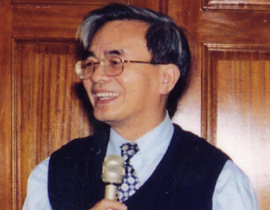
\includegraphics[scale=1]{Photos/phandinhdieu1}
\caption{Giáo sư Phan Đình Diệu}
\end{figure}
\begin{center}
Các bạn quan tâm có thể đọc:\\
\vspace{0.5cm}
Tuyển tập một số bài viết của GS. Phan Đình Diệu trên trang:\\
\vspace{1cm}
\centerline{\textcolor{C2}{\bf {\LARGE \href{http://www.phandinhdieu.net/accueil.html}{Nghĩ Suy Cùng Đất Nước}}}} 
 \vspace{1cm}
\url{http://www.phandinhdieu.net/accueil.html}
\end{center}

\newpage


%\fancyhead{}
%\thispagestyle{plain}
\begin{scriptsize}
%\textcolor{C1}{
\tableofcontents 
%}
\end{scriptsize}


%\part{Nghĩ Suy Cùng Đất Nước}
%\clearpage{\pagestyle{empty}\cleardoublepage}


\chapter{Viết về Anh, Giáo sư Phan Đình Diệu (Hà Huy Khoái)}
Nguồn: \href{https://tiasang.com.vn/khoa-hoc-cong-nghe/Viet-ve-anh-giao-su-Phan-Dinh-Dieu-12393}{Báo Tia Sáng}

\begin{figure}
\centering
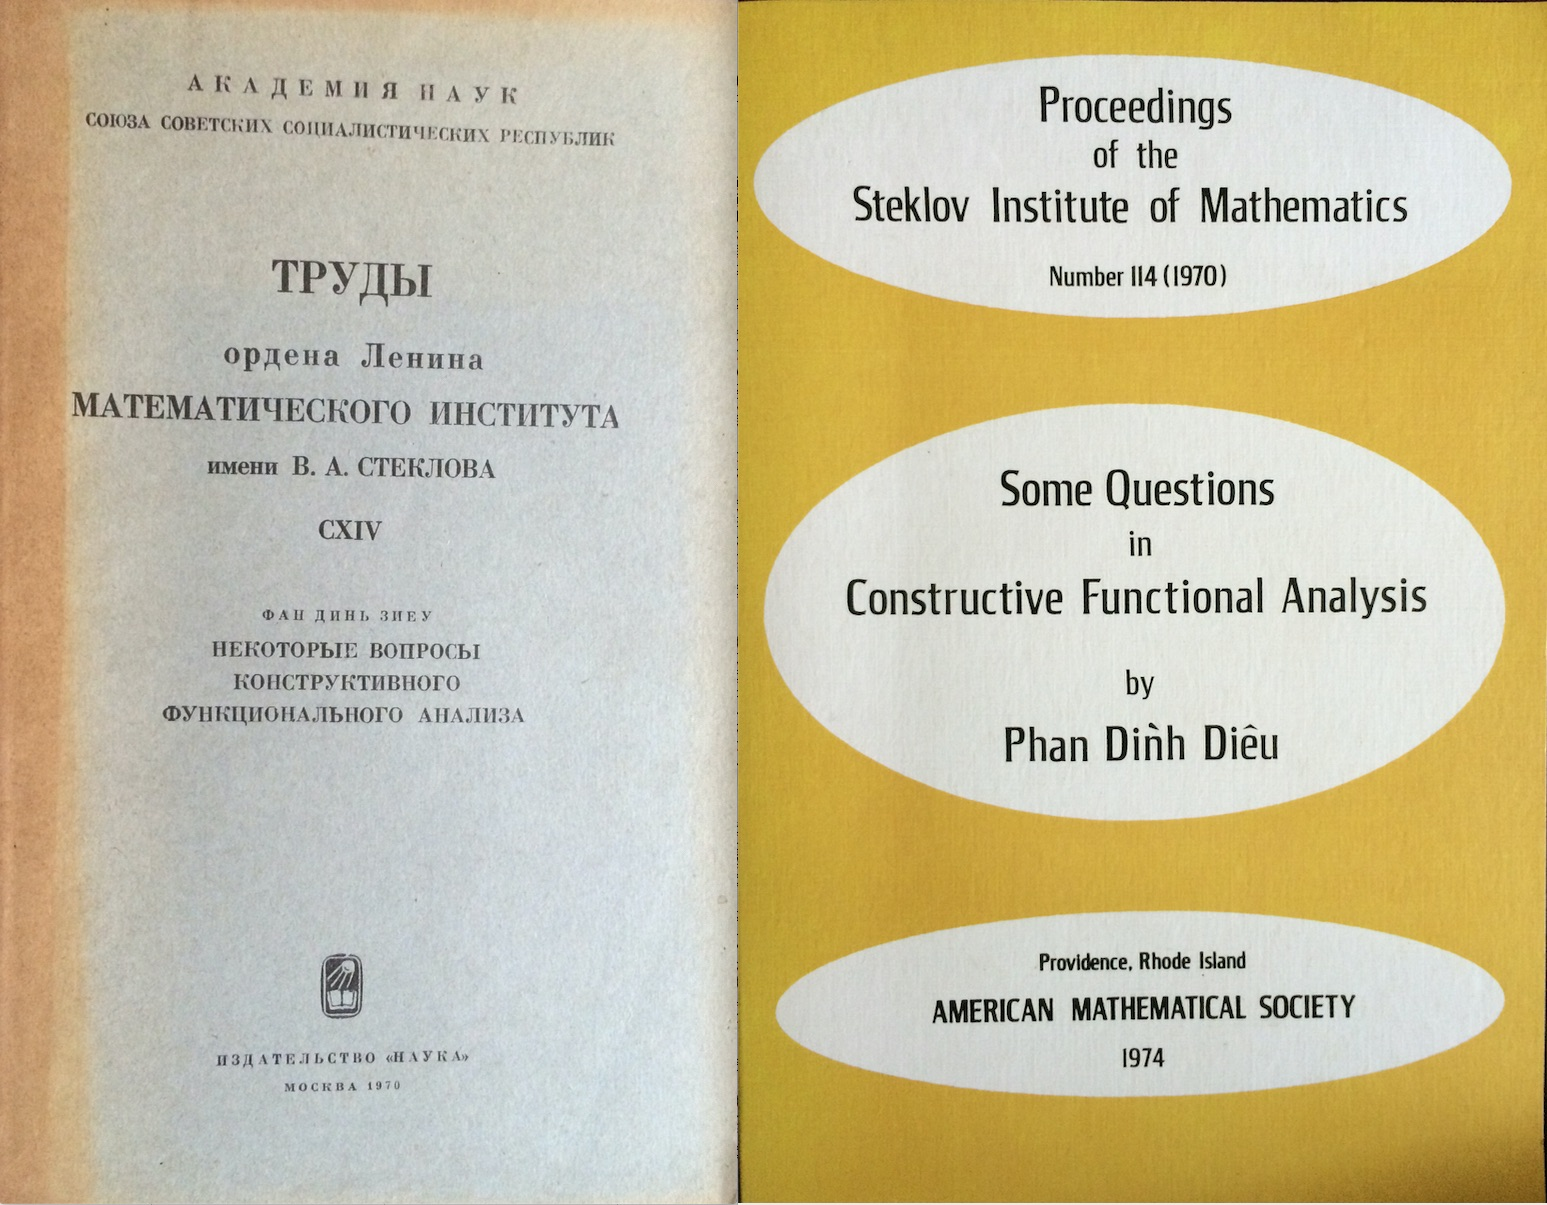
\includegraphics[scale=0.12]{Photos/DieuThesis}
\caption{Công trình về \textit{Giải tích hàm kiến thiết} của GS Phan Đình Diệu được in thành sách của Steklov Institute of Mathematics và sau đó được dịch sang tiếng Anh bởi American Mathematical Society. Xem thêm bài viết của GS Lê Tự Quốc Thắng ở phần \ref{LTQT} }
\end{figure}
Thế là Anh đã ra đi.

Mấy hôm nay trên báo chí, trên “cộng đồng mạng” tràn ngập những bài viết, những lời bày tỏ tình cảm với Anh. Ai cũng muốn viết gì đó về Anh.

Tôi cũng vậy.

Nhưng viết về Anh thật khó. Không thể nói những lời thừa. Không thể nói những lời mọi người đều đã nói. Con người Anh luôn độc đáo, sâu sắc, chính xác. Rất khó bỏ đi dù chỉ một từ nào đó trong những bài viết của Anh.

Anh độc đáo ngay từ khi chập chững vào làng Toán. Vì thích Số học mà Anh đã tự học tiếng Trung để dịch cuốn Số học của Hoa La Canh. Vì yêu thích sự chính xác mà anh chọn cho mình môn Logic khi đi làm nghiên cứu sinh ở Liên Xô. Chỉ trong 5 năm, anh đã xây dựng nên một ngành mới trong Toán học: Giải tích hàm kiến thiết. Công trình của anh được in thành sách (Some questions in constructive functional analysis. Proceedings of the Steklov Institute of Mathematics, No. 114 (1970). Translated from the Russian by J. M. Danskin.American Mathematical Society, Providence, R.I., 1974. iv+228 pp.). Chữ “kiến thiết” được dùng cho những ngành Toán mà ở đó không chấp nhận chứng minh phản chứng: không thể khẳng định một cái gì đó là “tồn tại” nếu điều giả thiết “nó không tồn tại” dẫn đến nghịch lý. Muốn chứng minh “tồn tại”, phải đưa ra thuật toán xây dựng (“kiến thiết”) nó.

Tư tưởng “kiến thiết” đó cũng làm Anh trở nên gần gũi với Khoa học máy tính một cách tự nhiên. Và với nhãn quan sáng suốt của mình, Anh nhận ra ngay từ những năm đầu của thập ký 70, thế kỷ trước, rằng Tin học chính là Khoa học của tương lai, và Việt Nam nhất thiết phải xây dựng ngành Tin học. Có thể nói rằng trình độ Tin học của Việt Nam thời kỳ đó cao hơn nếu so sánh với những nước trong vùng Đông Nam Á. Chúng ta đã từng đi trước, nhưng vì nhiều nguyên nhân nên đã tụt lại phía sau.

Đọc lại những bài viết của Anh về Khoa học, về con đường phát triển của xã hội Việt Nam, không thể không ngạc nhiên về những kiến giải sâu sắc, độc đáo, về tầm nhìn của anh. Sự phát triển, những vấn đề mà xã hội đang phải đối mặt gần như là “minh hoạ” những gì Anh nói đã vài chục năm. Và trên hết, ta cảm nhận tấm lòng Anh, một kẻ sỹ của thời đại mới, luôn trăn trở với con đường đi của đất nước.

Anh không chỉ là nhà khoa học, nhà tư tưởng, Anh là người say mê tất cả những gì thuộc về tri thức nhân loại. Tôi còn nhớ, Anh đã bình rất hay về cảnh đối đáp giữa Khuất Nguyên và Ngư Phủ trên sông Tương (trong một bài viết, hình như đăng trên báo Văn Nghệ). Những lần trò chuyện về Thơ, tôi thấy Anh rất thích Rabindranath Tagore, đặc biệt là những câu:

Đôi mắt lo âu của em buồn,\\
đôi mắt em muốn tìm vào tâm tưởng của anh\\
như trăng kia muốn vào sâu biển cả…\\

Trái tim anh cũng ở gần em,\\
như chính cuộc đời của em vậy\\
nhưng chẳng bao giờ em hiểu hết nó đâu.\\

Hình như Anh luôn có cảm giác người khác không hiểu hết mình. Mà đúng vậy. Anh sâu sắc quá, độc đáo quá, nghĩ xa hơn người khác nhiều quá, để người ta có thể hiểu hết về Anh. Nhưng dù không hiểu hết, Anh vẫn chiếm trọn tình yêu và lòng khâm phục của những người có dịp gần Anh.

Những lời sau đây của Tagore viết về Cái Chết, hình như cũng chính là dành cho Anh:

Khi nghĩ về những năm tháng đã qua,\\
đã trôi xuôi theo theo giòng chảy\\
của cuộc sống, và tình yêu, và cái chết,\\
tôi thấy sự ra đi vĩnh viễn là tự do biết bao.\\

Không cần phải nói lời cầu mong Anh yên nghỉ. Dường như Anh đã đi xa, để có thể được tự do suy tưởng. Một mình.


\chapter{Phan Đình Diệu đã sống một cuộc đời rất đàng hoàng (Nguyên Ngọc)}
Nguồn: \href{https://nguoidothi.net.vn/nha-van-nguyen-ngoc-phan-dinh-dieu-da-song-mot-cuoc-doi-rat-dang-hoang-39640.html}{Báo Người Đô Thị}

\begin{quote}
“Anh Diệu luôn trân trọng con người để luôn có được những ứng xử, chăm lo tinh tế nhất khiến chúng ta chỉ còn biết nói rằng, sống tử tế là phải như thế đấy, chơi với nhau là phải như thế…” - nhà văn lão thành Nguyên Ngọc nói về người bạn lớn của mình, cũng là người từng đồng hành cùng ông trong suốt một nhiệm kỳ làm Đại biểu Quốc hội (khoá VI): GS. Phan Đình Diệu, nhân kỷ niệm 5 năm ngày mất (13.5.2018) và 87 năm ngày sinh (12.6.1936) của nhà toán học, nhà khoa học máy tính nổi tiếng.
\end{quote}

{\bf “Cái tự do thơ thới ấy, nó rất gần với văn nghệ sĩ”}

\emph{Trước khi có một tình bạn thân thiết với GS. Phan Đình Diệu, ông từng quan sát nhà toán học ở cự ly nào?}

Năm 1988, khi tôi đang là Tổng biên tập báo Văn Nghệ, thì có một bài báo gửi đến toà soạn, ngắn thôi, chỉ khoảng tầm hơn 200 chữ, ký tên hai ông Phan Đình Diệu và Hoàng Tụy.

Nội dung bày tỏ mối băn khoăn của hai nhà khoa học hàng đầu về khái niệm “quay hộp đen” mà Tổng Bí thư thời kỳ ấy đã sử dụng trong một bài phát biểu đăng báo (thậm chí về sau còn thành tên chuyên mục của tờ báo ấy).

Tác giả bài báo cho rằng, đây là một cách vận dụng sai thuật ngữ và là một phép liên tưởng thiếu chính xác, do chưa hiểu thấu đáo về kiến thức chuyên ngành. Bài viết tuy ngắn kỷ lục và chỉ chiếm một ô nhỏ trên báo nhưng thực sự gây chấn động, khiến báo bạn sau đó phải bỏ hẳn chuyên mục đó.

Nhưng trước đó thì chúng tôi cũng đã quen biết nhau, đặc biệt là khi cùng tham gia Quốc hội khóa VI (1976 - 1981), thuộc Ủy ban Văn hóa Giáo dục của Quốc hội.

Ở vào cái thời mà hội trường Quốc hội chưa có bấm nút, chưa có chất vấn Đại biểu Quốc hội… thì những tiếng nói phản biện đã cất lên trong bối cảnh thế nào?

Diễn đàn Quốc hội bấy giờ thì gần như không có tiếng nói phản biện, riêng Phan Đình Diệu luôn là người đầu tiên đưa ra những ý kiến trái chiều. Anh Diệu thường nói nhiều về việc cần lắng nghe ý kiến của trí thức, đặc biệt là vấn đề dân chủ.

Thường trong nhóm chúng tôi hồi đó, những ý kiến của các anh Phan Đình Diệu, Tạ Quang Bửu… bao giờ cũng là những ý kiến rất sâu sắc và đáng lắng nghe. Ba anh em chúng tôi hồi đấy cũng chơi thân nhau nên cũng bàn được với nhau nhiều việc, nhiều chuyện.

Là một nhà toán học nhưng anh Diệu có mối quan tâm rộng lắm, anh cũng đặc biệt quan tâm đến văn hóa. Hồi Thủ tướng Võ Văn Kiệt còn sống, ông từng gợi ý cho tôi là nên thành lập một viện nghiên cứu tư nhân về văn hóa, và người đầu tiên tôi nghĩ ngay tới không ai khác chính là GS. Phan Đình Diệu. Hai anh em cũng đã bàn đến việc nếu làm nghiên cứu về văn hóa thì nên làm thế nào để văn hóa gắn liền với giáo dục, làm sao để tạo ra được một cái phanh cho vấn nạn văn hoá đang xuống cấp trầm trọng… 

\emph{Đó có phải là một trong những lý do khiến GS. Phan Đình Diệu trở thành một cái tên có sức hút mạnh với giới văn nghệ sĩ?}

Lý do trước hết, theo tôi, anh Diệu là một con người rất đàng hoàng. Anh thực sự đã sống một cuộc đời rất đàng hoàng, với tất cả sự thẳng thắn và trung thực. Cái tự do thơ thới ấy, nó rất gần với giới văn nghệ sĩ.

Anh Diệu cũng là người làm thơ rất hay, có một bài thơ anh làm tặng GS. Trần Đại Nghĩa tôi rất thích: ...Tình nặng ấy chưng tình đất nước/Nghiệp đời há kể nghiệp vàng son...

Con người đó là người rất hiểu thơ và rất hiểu văn học, vì thực ra toán học nó rất gần với văn học. Tôi vẫn hay nói với các anh em trẻ, nhất là mấy anh em trẻ viết văn, là một trong những nhược điểm của các bạn là ít quan tâm đến khoa học tự nhiên quá, trong khi khoa học tự nhiên, chẳng hạn như toán học, cái sức tưởng tượng của nó ghê gớm lắm (con tôi cũng làm toán nên tôi biết), vì thế nó rất gần với văn học nghệ thuật. Tôi với anh Diệu dễ gần nhau, thân nhau chắc cũng là vì thế.


\emph{Điều gì đã làm nên sự đàng hoàng đó, theo ông?}

Tính cách Nghệ là một phần, cái nôi địa linh nhân kiệt là một phần. Phần nữa, quan trọng không kém, là thế hệ của chúng tôi đã may mắn được hưởng một nền giáo dục phải nói là rất đàng hoàng, với những ông thầy “ghê gớm”, có sức ảnh hưởng rất lớn tới học trò. Thế hệ bọn tôi được một cái điều như thế!

\emph{Dường như lâu lắm tôi mới nghe đến ba chữ tưởng như rất quen tai này: “sống đàng hoàng”. Theo ông, thế nào là “sống đàng hoàng”?}

Nó thật ra rất đơn giản, nó đến từ sự tử tế. Anh Diệu luôn trân trọng con người để luôn có được những ứng xử, chăm lo tinh tế nhất khiến chúng ta chỉ còn biết nói rằng: Sống tử tế là phải như thế đấy, chơi với nhau là phải như thế…

Anh Diệu là người sống rất tình cảm. Tôi nhớ anh từng kể với tôi, thời Cải cách ruộng đất, có lần anh thấy người ta giải một “tên địa chủ”, lại gần thì hóa ra là ông thầy mà anh ấy rất kính trọng, thế là cậu học trò ấy cứ đứng đấy khóc mãi. Tận tới sau này khi kể lại cho tôi nghe, anh còn ứa nước mắt. Cái ấn tượng đó hẳn đã hằn rất sâu trong tâm trí anh Diệu để sau này góp phần hình thành nên cái con người cương trực và tử tế nơi anh.

Anh Diệu, tôi nghĩ anh ấy là một trí thức lớn đúng nghĩa.


{\bf “Sự nhất quán ấy không dễ gì mà có được”.}

\emph{Thế nào là một “trí thức lớn đúng nghĩa”, theo ông? }

Trí thức theo tôi không chỉ là người học cao đâu, có nhiều người học rất ghê, nhưng người ta cũng chỉ có thể gọi họ là nhà bác học, chứ không phải là một bậc trí thức. Trí thức, nói một cách nôm na, còn phải là những người “giữa đường thấy sự bất bằng chẳng tha”; hay như từ của anh Cao Huy Thuần, là mấy người hay xớ rớ vào việc người khác, rằng việc đó không ảnh hưởng gì tới họ, nhưng họ vẫn thấy mình liên quan, mình cần có trách nhiệm tới cùng.

Nhiệm vụ của trí thức theo tôi là làm cho xã hội không được yên, không thể đứng yên, theo cái nghĩa tích cực của điều này.

\emph{Hiểu theo nghĩa đó, ông thấy xã hội Việt Nam đương đại trong mấy thập niên gần đây có được nhiều bậc trí thức? Và ông, có định vị mình là trí thức?}

Cũng có, ông Phan Đình Diệu là trí thức, ông Hoàng Tụy cũng là trí thức…, còn những người khác nữa. Tôi cũng là người trí thức, vì tôi toàn đi nói những cái chuyện có dính gì đến tôi đâu, mà đời tôi cũng chẳng cần cái gì khác ngoài cái đời sống bình thường như thế này.

\emph{Ở thời điểm bản lề trước và sau Đổi mới, khi báo Văn Nghệ (mà có thời gian ông làm Tổng biên tập) lần lượt đăng những truyện ngắn gây chấn động văn đàn của Nguyễn Huy Thiệp hay bút ký nổi tiếng Cái đêm hôm ấy… đêm gì của Phùng Gia Lộc…, thì tại diễn đàn Quốc hội (các khoá V, VI) hay Mặt trận Tổ quốc Việt Nam (các khoá III, IV, V, VI, VII), GS. Phan Đình Diệu cũng được biết là một tiếng nói phản biện đầy nhiệt thành và nhiều trăn trở. Ông nghĩ, đó là do “thời thế tạo anh hùng”, hay chính là ngược lại?}

Thực ra thì hồi đó bọn mình cũng có tranh thủ được một thời gian để kịp nói ra được những gì cần nói. Thế nhưng để có được một tiếng nói xuyên suốt, cả trong những thời điểm không thuận lợi, thì đấy còn là bản lĩnh và tầm nhìn.

Tôi thì thật ra cũng không hiểu được hết các bước trưởng thành của một tiếng nói đâu, vì với mỗi người, các bước ấy nó rất khác nhau. Có người đi nhanh hơn, nhìn thấy được sớm hơn và đáng kể, là cất được tiếng nói sớm hơn. Những tiếng nói ấy mạnh lắm, và đó là sức mạnh tự thân của họ.

Một tiếng nói như Phan Châu Trinh chẳng hạn, nó lạ lắm, tận giờ chúng ta vẫn chưa thể hiểu hết được ông ấy đâu, mấy mươi năm nay tôi cứ nghĩ mãi về cái ông Phan Châu Trinh này, rất khó hiểu vì sao lúc đó ông ấy lại có thể xuất sắc đến thế. Nhưng ông ấy cũng là một người vô cùng cô độc. Tôi nghĩ anh Diệu, anh ấy hiểu rất rõ những điều đó.  

Còn như tôi đây chẳng hạn, tôi nói thật là các bước của tôi nó cũng chậm lắm, cái giai đoạn mà tôi giáo điều nó cũng kéo dài lắm. Phải mãi đến tận năm 1979, khi sang Campuchia và tận nhìn tận thấy, tôi mới sực nhận ra, khi cái gọi là “cá nhân con người” bị đổ đồng, bị xóa sổ, bị thay thế bởi cái “chủ nghĩa bầy đàn”… thì nó có thể khủng khiếp đến thế nào.

Thế nên khi về tôi mới quyết làm cái Đề dẫn năm 1979 như sau này mọi người vẫn hay nhắc đến. Anh em văn nghệ sĩ hồi đấy hào hứng lắm, anh Diệu cũng biết chuyện bọn tôi làm cái Đề dẫn đó, và ủng hộ…

\emph{
Nhìn thấy sớm là một chuyện, nhưng hơn hết, còn là sự nhất quán, khi trước giờ vốn không thiếu những tiếng nói “linh hoạt”, “gió chiều nào xoay chiều nấy”…?}

Thực ra mà nói, cái phẩm chất đó của con người, cái sự nhất quán đó của con người, cũng không dễ gì có được, mà đôi khi không phải do họ muốn thế, tính thế. Có thể có lúc mình không biết mình sai, đời tôi sai nhiều lắm chứ, nhưng có điều mình sai một cách trung thực; mình cũng có lúc giáo điều, nhưng mình giáo điều một cách trung thực…

Anh Diệu thì khác, anh ấy có được cái sự nhất quán đó.

\emph{Ông nghĩ vì sao một tiếng nói trái chiều như Phan Đình Diệu vẫn có thể vang lên một cách dõng dạc tại các diễn đàn chính thống trong suốt một thời gian dài, dù không “dễ nghe” chút nào?}

Ở anh Diệu, anh ấy có một chữ “Liêm” rất rõ ràng, cái mục đích lên tiếng của anh ấy nó vô cùng trong sáng. Anh chỉ đơn giản là người dám nói lên sự thật thôi, còn nhiều người khác thì không dám. Anh nói rất chặt chẽ và đàng hoàng, lịch sự; không đả kích cá nhân, cũng không nói sau lưng hay bên lề. Một người đứng đắn, đàng hoàng, có uy tín quốc tế như thế, người ta phải nể chứ! 

Lê Quân thực hiện

\chapter{Anh Diệu (Hồ Tú Bảo)}
Nguồn: \href{https://www.tiasang.com.vn/-khoa-hoc-cong-nghe/Anh-Dieu-12410}{Báo Tia Sáng}
\begin{figure}
\centering
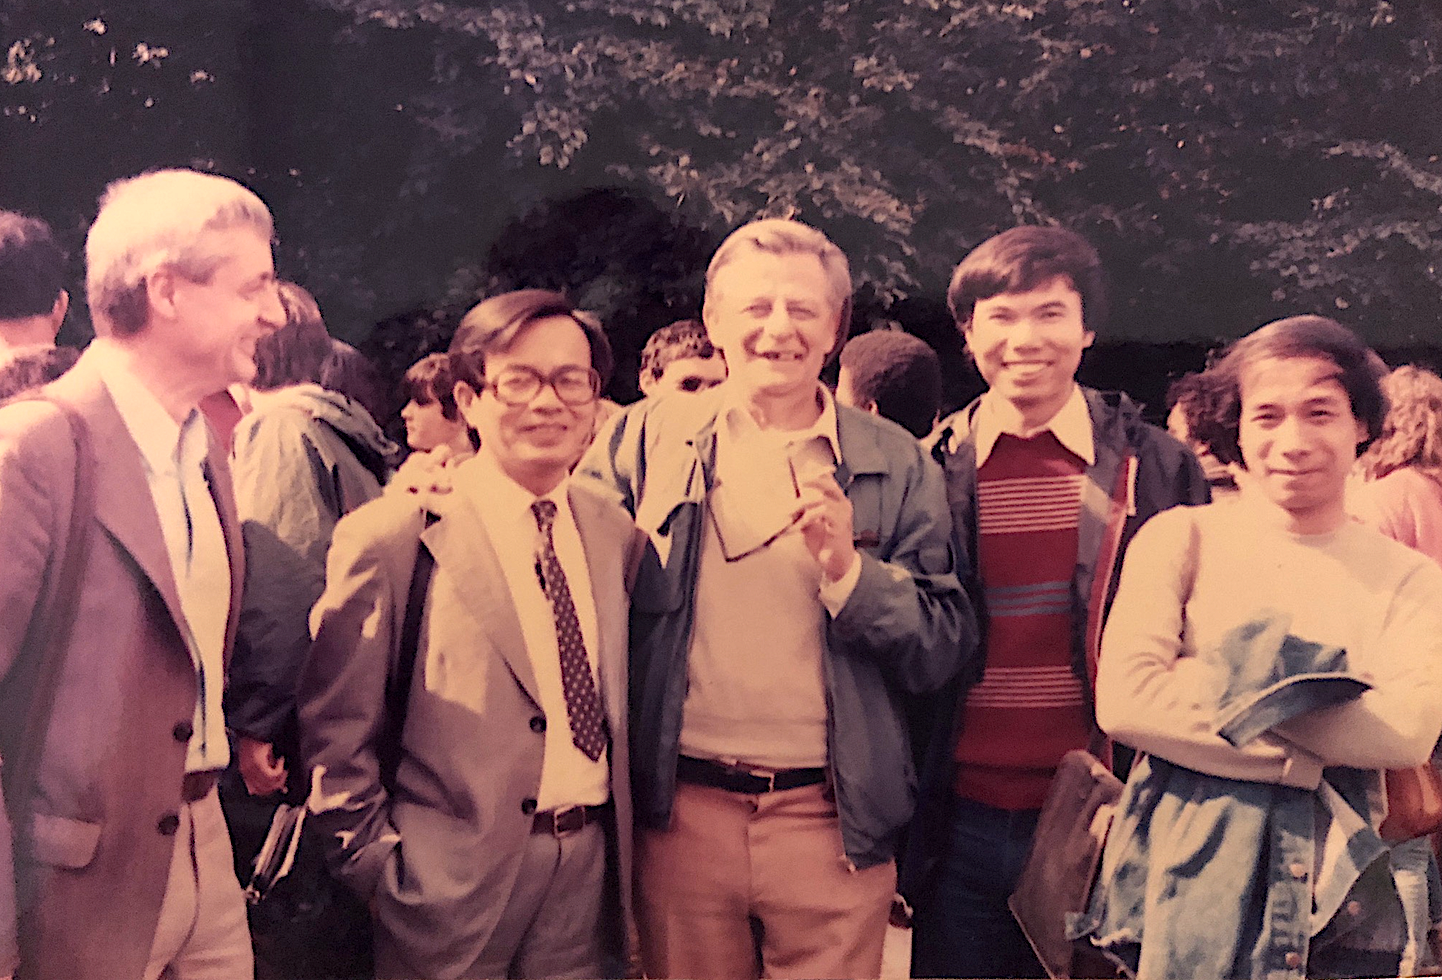
\includegraphics[scale=0.3]{Photos/Alain}
\caption{Từ trái qua: Kỹ sư Alain Teisonnière, anh Diệu, giáo sư Henri van Regemortor, Đặng Văn Đức và Hồ Tú Bảo (hai cán bộ của Viện) tại hội chợ Báo Nhân Đạo (l’Humanité), Paris 1985. Nguồn: Hồ Tú Bảo. }
\end{figure}


Xin được gọi anh là một hào kiệt và người anh cả của tin học Việt Nam.


Đúng nửa thế kỷ trước chúng tôi là những cô bé cậu bé lớp chuyên toán của Trường Đại học Sư phạm Hà Nội, sơ tán ở làng Viên Nội bên bờ sông Đáy. Mỗi chiều muộn thứ bảy lại thấy một người đẹp trai đạp xe về Viên Nội thăm vợ là cán bộ đi học ở Khoa Toán mới sinh con. Mọi người bảo nhau đấy là nhà toán học Phan Đình Diệu, mới tốt nghiệp tiến sĩ khoa học ở Liên Xô về nước. Hồi ấy số tiến sĩ khoa học của cả nước chỉ đếm trên đầu ngón tay. Sáng chủ nhật thấy nhà toán học mang một chậu quần áo tã lót đi giặt, rồi gánh nước từ giếng làng về đổ bể như lũ học trò chúng tôi.

Câu chuyện tuổi thơ ấy bẵng đi chục năm khi tôi đang học dở ngành toán thì đi lính,có những ngày Quảng Trị hè 1972, bị thương và về học tiếp chương trình đại học ngành toán ứng dụng. Ra trường, người bạn thân đang làm ở Viện Khoa học Tính toán và Điều khiển của Viện Khoa học Việt Nam, nay là Viện Hàn lâm KH\&CN Việt Nam, rủ tôi xin về Viện và dẫn đến gặp Viện trưởng. Gặp lại anh, người gánh nước cùng chúng tôi năm xưa.

Xem tên các môn học rất mới của Khoa Toán-Lý Bách Khoa hồi đó, hỏi về luận án tốt nghiệp và khen học tốt, anh đồng ý nhận tôi về Viện. Ít ngày sau tôi thành một “viện sĩ” như tụi tôi vẫn đùa (cũng lúc ấy có chuyện một cô gái tốt nghiệp ở Đức về, mang lá thư của người bác đang làm Bộ trưởng đến đề nghị anh Diệu nhận về Viện, anh đã dứt khoát từ chối).

Có một thời gian dài là “quân anh Diệu”, nhớ và nghĩ về anh tôi thấy rõ mấy điều sau.

1. Sự dấn thân của anh Diệu vào lĩnh vực tin học (còn được gọi với các tên công nghệ thông tin hay khoa học máy tính). Theo quan sát của tôi, mỗi lĩnh vực khoa học ở mỗi quốc gia có những người vượt trội trong quãng thời gian một vài chục năm. Đó là những người có tài năng xuất chúng và có sự phấn đấu bền bỉ. Trong toán học Việt Nam đó là các giáo sư Lê Văn Thiêm, Hoàng Tuỵ, rồi nhiều năm sau là Ngô Bảo Châu… Trong tin học tôi nghĩ đấy là anh Diệu.

Trong những năm đầu nghiên cứu toán anh Diệu đã đạt những kết quả rất xuất sắc, và tôi tin anh sẽ làm được rất nhiều nữa nếu tiếp tục con đường này. Nhưng trong những năm tháng chiến tranh ấy chúng ta đã có những chiếc máy tính lớn Minsk 22 của Liên Xô, ODRA 1304 của Ba Lan… và cần dùng chúng cho các nhiệm vụ quốc gia. Được giao trọng trách xây dựng và phát triển ngành tin học, anh Diệu đã dành hầu hết thời gian để tự học và nghiên cứu về tin học, một lĩnh vực mới rất đa dạng và phong phú.

Khác với toán học nơi người làm toán thường nghiên cứu độc lập và có thể chỉ cần bút và giấy, tin học vừa có phần lý thuyết luôn thay đổi rất nhanh, vừa gắn với công nghiệp máy tính (phần cứng), vừa gắn với phát triển các thuật toán và chương trình (phần mềm), và vừa gắn với các hệ thống ứng dụng (ở ta hồi đó là những nhiệm vụ tính toán khoa học trong khí tượng và địa chất…). Dân tin học cũng thường không làm việc độc lập, mà phải liên kết trong cácnhóm. Người phụ trách tin học bắt buộc phải đọc và học nhiều kiến thức khác nhau, thường xuyên thay đổi. Phải có niềm ham mê đặc biệt và một trí lực phi thường mới có thể đọc và hiểu được nhiều thứ như vậy, để có thể dẫn dắt một tập thể, để có thể chia sẻ và thuyết phục một cộng đồng. Và anh Diệu đã làm như vậy.

Kiên định với những quan điểm riêng là điều luôn nhất quán ở anh Diệu.

Trong quỹ thời gian hạn chế, anh Diệu vẫn làm nghiên cứu về toán. Anh viết bài về mật mã, về lập luận xác suất… Anh viết sách về lý thuyết automat và thuật toán, sách về logic toán. Hơn mười năm trước tôi có dịp mời anh thăm Viện Khoa học và Tiên tiến Nhật Bản và trao đổi với giáo sư Ono, chuyên gia hàng đầu về logic toán của Nhật. Câu chuyện của hai vị giáo sư tuổi bảy mươi sôi nổi, sâu sắc, đầy thú vị và uyên bác.

Với anh Diệu, tôi hiểu việc gác lại con đường làm toán để dành tâm sức cho sự phát triển nền tin học nước nhà từ thuở sung sức của đời làm khoa học là một lựa chọn đúng đắn. Anh làm được nhiều hơn cho cộng đồng và đất nước.

2. Tầm nhìn sâu rộng của anh Diệu và những đóng góp của anh về chính sách phát triển tin học quốc gia. Tiêu biểu nhất là ba lần anh Diệu chủ trì việc xây dựng chương trình quốc gia về công nghệ thông tin.

Ngay từ khi mới đi làm tôi đã có dịp xem tập tài liệu rất dầy do anh Diệu và anh Trần Lưu Chương (khi đó phụ trách Cục máy tính của Bộ Khoa học và Công nghệ) viết xong vào năm 1976. Tài liệu này trình bày bức tranh tổng thể về tin học trên toàn thế giới và đề xuất kế hoạch phát triển ngành tin học Việt Nam. Vào năm 1976 sinh viên tụi tôi vẫn lập trình trên các băng từ đục lỗ, thì một chương trình chi tiết như vậy cho thấy người viết đã có tầm nhìn rất xa và cái nhìn đã rõ khi vạch con đường của tin học Việt Nam.

Nhưng đề xuất năm 1976 này đã chưa được phê duyệt. Trong các năm 1981 và 1982, dưới sự chỉ đạo tâm huyết của anh Diệu, nhóm các nhà khoa học trẻ của Viện Khoa học Tính toán và Điều khiển đã thiết kế và chế tạo chiếc máy vi tính mẫu đầu tiên của Việt Nam, như một trong những chiếc máy vi tính được chế tạo sớm ở châu Á. Vào năm 1984 khi Việt Nam vẫn đang bị cấm vận, anh Diệu lại chủ trì đưa ra một bản mới của chương trình. Vẫn thường được xem là những chiếc máy và chương trình "đẻ non" khi xã hội chưa sẵn sàng, cácbước đi đầu này đã dẫn đến những bước đi tiếp theo.

Không nao núng với hai lần chưa thành công trước đó, anh Diệu- người chấp bút không mỏi mệt- đã có một bản dự thảo của chương trình được phê duyệt vào mùa hè 1994 theo Nghị định 49/CP, và từ đó một chương trình quốc gia về công nghệ thông tin đã được tiến hành.

Năm 1984 khi tôi học xong DEA (chương trình thạc sĩ ở Pháp) về xử lý ảnh và chuẩn bị tiếp tục làm luận án theo hướng này. Trong một bức thư gửi từ Việt Nam qua anh Diệu viết “nếu có thể Bảo nên chuyển qua làm về trí tuệ nhân tạo vì đấy là tương lai của tin học”. Theo lời anh tôi đã chuyển hướng, dù mất công hơn vì chưa biết gì về chuyện này. Bây giờ sau hơn ba chục năm, trí tuệ nhân tạo ngày càng có vai trò thiết yếu trong thời chuyển đổi số, càng thấy tầm nhìn của anh.

3. Những ý kiến đóng góp của anh Diệu về xây dựng đất nước. Là người luôn trăn trở, suy nghĩ về những vấn đề của phát triển đất nước, anh Diệu đã luôn thẳng thắn nêu những chính kiến của mình.

Đấy là những ý kiến anh phát biểu tại Quốc hội, tại Mặt trận Tổ quốc Việt Nam khi anh là thành viên của các tổ chức này. Đấy là các ý kiến khi anh gặp các lãnh đạo cấp cao của Đảng cộng sản và nhà nước. Đấy là các bài viết đầy tâm huyết và trăn trở về con đường phát triển đất nước. Kiên định với những quan điểm riêng là điều luôn nhất quán ở anh Diệu.

4. Mối quan hệ chân tình của anh Diệu với bạn bè và đồng nghiệp. Trong quan sát của tôi, bạn bè nước ngoài đến làm việc ở Việt Nam đều tỏ rõ sự quý trọng với anh. Đó là các nhà triết học của Viện Hàn lâm Nga khi đến Việt Nam đã duy nhất mời anh Diệu viết với họ về triết học trong khoa học, là giáo sư Henri van Regemorter và kỹ sư Alain Teissonnière từ Pháp khi giúp ta phát triển tin học, là vợ chồng nhà toán học Đức Klaus và Angela Krickerberg sang dạy về dịch tễ học, là giáo sư Judy Ladinsky giúp ta xây dựng hợp tác khoa học Mỹ-Việt từ khi đất nước bị cấm vận… Anh Diệu cũng được các anh chị Việt kiều rất quý trọng, và nhiều người đã về giúp Việt Nam theo lời mời của anh. Tôi thấy hầu hết những người làm việc cùng đều quý trọng anh. Anh Diệu không lấy lòng người khác, mà bằng trí tuệ và nhân cách, bằng công việc chung, bằng sự chân tình, anh thu phục lòng người. Với những người trẻ hơn như tụi tôi, anh còn có nhiều chia sẻ, chỉ dẫn ân cần.

Tôi tự hỏi nếu chỉ dùng một vài từ để nói về anh Diệu, sẽ là gì?

Hồi nhỏ tôi mê mẩn “Lá cờ thêu sáu chữ vàng” của nhà văn Nguyễn Huy Tưởng viết về Trần Quốc Toản với hình ảnh của “sáu trăm gã hào kiệt”, và nhớ đến cả nước đã trân trọng gọi Đại tướng Võ Nguyên Giáp là “người anh cả của quân đội nhân dân Việt Nam”. Với anh Diệu, xin được gọi anh là một hào kiệt và người anh cả của tin học Việt Nam.

Năm 1954 sau ngày hoà bình lập lại ở miền Bắc, vừa học xong phổ thông ở quê Hà Tĩnh, như nhiều chàng trai trẻ miền Trung đầy nghị lực, anh Diệu đi bộ ra Hà Nội thi vào trường Đại học Khoa học, rồi theo học trường Đại học Sư phạm Hà Nội. Tốt nghiệp thủ khoa ngành Toán, anh tham gia giảng dạy ở đây 5 năm cho đến 1962 được cử đi làm nghiên cứu sinh về Toán ở trường Đại học Tổng hợp Moscow. Lĩnh vực nghiên cứu lúc đó của anh Diệu là toán học kiến thiết. Nói nôm na, đây là lĩnh vực nhằm không những chỉ ra các sự “tồn tại” trong toán học mà còn chỉ ra liệu “ta có thể xây dựng” được chúng với các thuật toán. Luận án tiến sĩ khoa học của anh Diệu dựa trên sáu bài báo anh đăng trên tạp chí “Doklady Akademii Nauk” nổi tiếng ở Nga, sau được in trong cuốn sách “Một số câu hỏi về giải tích hàm kiến thiết” ở Nga và ở Mỹ. Năm 1967 sau khi bảo vệ luận án tiến sĩ khoa học, anh Diệu về nước tham gia xây dựng Phòng Toán học Tính toán của Ủy ban Khoa học và Kỹ thuật Nhà nước, tiền thân của Viện Khoa học Tính toán và Điều khiển (cũng như các Phòng Toán học, Phòng Vật Lý... là tiền thân của Viện Toán học, Viện Vật lý... của Viện Khoa học Việt Nam).

\chapter{GS Phan Đình Diệu: Tâm và Tầm của Trí Thức Việt (Hiệu Minh)}
\input{BaiViet/GiangCongThe.tex}

\chapter{Giáo sư Phan Đình Diệu: Khí phách và Trí tuệ (Trương Huy San)}
%GIÁO SƯ PHAN ĐÌNH DIỆU (1936-2018): KHÍ PHÁCH \& TRÍ TUỆ (Trương Huy San)
 
Nguồn: \href{http://nghiencuuquocte.org/forums/topic/giao-su-phan-dinh-dieu-1936-2018-khi-phach-va-tri-tue/}{Báo Nghiên cứu quốc tế} 
và \href{https://www.facebook.com/Osinhuyduc/posts/1620411811327327}{Facebook của tác giả} 




Sáng nay tôi hỏi 5 bạn sinh trong thập niên 1980s, 3 bạn nói không biết GS Phan Đình Diệu. Tôi buồn nhưng không bất ngờ. Ông là một người mà thế hệ chúng tôi ngưỡng mộ, cả về tài năng và sự chính trực. Có lẽ vì sự chính trực ấy mà ông rất ít khi có mặt trên những bục vinh quang. Nhưng, những đóng góp thầm lặng của ông đặc biệt là trong vai trò đưa công nghệ thông tin vào VN đang ảnh hưởng lên cả những thế hệ không còn biết ông là ai nữa.
 

 
GS Phan Đình Diệu là một trong những người đầu tiên gầy dựng ngành khoa học tính toán của miền Bắc (1968). Chiếc máy vi tính đầu tiên, có thể coi là của Châu Á, ra đời năm 1980 [được thiết kế với chip Intel 8080A nên được đặt tên là VT80] là từ phòng thí nghiệm Viện Tin học của ông, bắt đầu từ những hợp tác trước đó với Viện Kỹ thuật Quân sự có sự giúp sức cả về chuyên môn và vật chất của ông André Trương Trọng Thi, người được coi là cha đẻ của máy tính cá nhân.

Theo tiến sỹ Vũ Duy Mẫn: “Năm 1981, sau khi lắp ráp thành công máy vi tính VT81 và cài đặt được ngôn ngữ lập trình Basic, Viện quyết định thử nghiệm đưa máy vi tính ứng dụng vào quản lý xí nghiệp cỡ nhỏ và vừa ở Xí nghiệp máy may Sinco”.

Nhưng, cho dù có nhiều nỗ lực, ngành công nghiệp sản xuất máy tính chỉ dừng lại ở đó. Tin học là một ngành không thể phát triển trong một quốc gia tự đóng cửa về chính trị và bị cô lập về thương mại với thế giới bên ngoài. Rất tiếc là khi tình hình trong nước bắt đầu cởi mở hơn thì GS Nguyễn Văn Hiệu được đưa lên thay giáo sư Trần Đại Nghĩa, làm Viện trưởng Viện khoa học Việt Nam. Năm 1993, ông Hiệu loại GS Phan Đình Diệu khi ngành tin học Việt Nam cần một người lãnh đạo có tâm và có tầm nhất.
GS Hiệu năm ấy 45 tuổi. Ông có mọi ưu đãi của Chế độ, từ kinh phí nghiên cứu tới quyền hạn. Nắm Viện, ông Hiệu kêu gọi “các anh các chị hãy tự cứu mình”. Các công ty được thành lập, Viện khoa học Việt Nam nhanh chóng trở thành một nơi “nửa hàn lâm, nửa chợ trời”[theo TS Giang Minh Thế]. Hàng nghìn cán bộ tài năng trôi giạt khắp nơi. Nền tin học Việt Nam chuyển một cách dứt khoát sang nghề… buôn máy tính.
Dù GS Phan Đình Diệu là người viết đề cương thành lập viện Công nghệ thông tin theo mô hình mới và khi bỏ phiếu thăm dò, ông nhận được tín nhiệm của đa số tuyệt đối, GS Nguyễn Văn Hiệu vẫn chọn một người có số phiếu thấp hơn vì lý do “biết làm kinh tế”. GS Phan Đình Diệu tuyên bố từ chức Viện phó Viện Khoa học Việt Nam và ra khỏi biên chế, những chuyên gia trẻ hết lòng vì khoa học như Nguyễn Chí Công, Vũ Duy Mẫn, Lê Hải Khôi, Giang Công Thế… bắt đầu phiêu bạt.

Cho dù vậy, theo GS Chu Hảo – thứ trưởng Bộ Khoa học Công nghệ thời kỳ internet được đưa vào VN – “GS Phan Đình Diệu vẫn là linh hồn của các chính sách phát triển công nghệ thông tin của nước ta”. Ông là Chủ tịch hội Tin học và là Phó Chủ tịch Uỷ ban Quốc gia phát triển Công nghệ Thông tin cho tới năm 1998.
Nếu như, GS Nguyễn Văn Hiệu nổi tiếng là một người biết sử dụng khoa học để làm chính trị và leo lên tới các đỉnh cao danh vọng thì GS Phan Đình Diệu lại là một con người mà ngay cả trong chính trị cũng chỉ tham gia với tinh thần khoa học.

Theo ông Trần Việt Phương – thư ký riêng của Thủ tướng Phạm Văn Đồng – từ đầu thập niên 1960s, khi được Thủ tướng Phạm Văn Đồng hỏi, GS Phan Đình Diệu đã cho rằng, hệ thống kinh tế Xô Viết sẽ sụp đổ nếu tiếp tục vận hành như thế này[Hy vọng là Trung tâm Lưu trữ quốc gia vẫn còn giữ được ý kiến này của GS Phan Đình Diệu].

Rất có thể, quyết định không bổ nhiệm GS Phan Đình Diệu vào năm 1993 của ông Hiệu còn có “lý do chính trị”. Từ năm 1989, GS Phan Đình Diệu có nhiều phát biểu về “đa nguyên” và đặc biệt là các ý kiến thẳng thắn của ông góp ý cho Hiến pháp 1992.

Tháng 10-1988, sau khi giải quyết xong vấn đề “đa đảng”[giải tán hai đảng Dân chủ và Xã hội], Tổng bí thư Nguyễn Văn Linh bắt đầu “chống đa nguyên” nhắm vào ông Trần Xuân Bách. Tháng 3-1989, Hội nghị Trung ương 6 khẳng định “Không chấp nhận chủ nghĩa đa nguyên”. Ngay sau đó trên báo Đảng, cả Trưởng ban Tuyên huấn Trung ương Trần Trọng Tân lẫn “nhà nghiên cứu” Trần Bạch Đằng đều có bài, trên tinh thần “Mác Xít”, nhấn mạnh rằng, “Nếu hiểu đa nguyên theo nghĩa triết học thì từ lâu đã bị phê phán là sai lầm. Chúng ta không chấp nhận”.

Ngày 15-8-1989, GS Phan Đình Diệu có bài trên Sài Gòn Giải Phóng, đáp trả các luận điệu trên đây. Ông cho rằng, muốn “tìm đường đi cho đất nước trong thế giới hiện đại” thì phải “vận dụng trí tuệ của thời đại” từ “nhiều nguồn tri thức”. Theo ông, “Những gì xảy ra trong thế kỷ hai mươi là điều không thể hình dung đối với những bộ óc, dù là vĩ đại, của giữa thế kỷ mười chín”.

Sau khi đọc bài của Giáo sư Phan Đình Diệu, từ Hà Nội, Bí thư Trần Xuân Bách gửi cho TBT Sài Gòn Giải Phóng Tô Hoà một tấm danh thiếp, mặt sau ghi: “Chuyển giùm anh Phan Đình Diệu, tôi ca ngợi bài này”. Đây là bài báo cuối cùng mà Tô Hoà cho đăng với tư cách tổng biên tập Sài Gòn Giải Phóng. Ngày 28-3-1990, Trung ương cách chức ông Trần Xuân Bách.

Hai năm sau, ngày 12-3-1992, trong một phiên họp góp ý cho Hiến pháp 1992, GS Phan Đình Diệu đã có một phát biểu rất gây tiếng vang ở Uỷ ban Trung ương MTTQ Việt Nam. Ông đề nghị “tạm gác lại” việc đưa vào Hiến pháp các thuật ngữ “chủ nghĩa xã hội, chủ nghĩa Marx – Lenin”. Ông đề nghị phải dũng cảm để thấy rằng, “mô hình CNXH, cũng như Marx – Lenin không còn đáp ứng được mục tiêu phát triển đất nước trong giai đoạn hiện nay”. Giai đoạn xây dựng một “tổ quốc Việt Nam trên tinh thần đoàn kết, hoà hợp và tự cường”.
Theo GS Phan Đình Diệu thì Việt Nam dứt khoát phải có “nhà nước pháp quyền”, chứ không thể tiếp tục “chuyên chính vô sản” hay “pháp quyền nửa vời”. Đặc biệt, ý kiến của ông về Mặt trận và các đoàn thể cho tới ngày nay vẫn còn rất thiết thực. Ông đề nghị, Hiến pháp chỉ cần coi lập hội là quyền tự do của người dân; từ bỏ việc nhà nước hoá các đoàn thể. Ông kêu gọi các đoàn thể thay vì dựa dẫm vào nhà nước phải lấy quần chúng làm gốc rễ, các cơ quan đảng, đoàn thể không ăn lương từ ngân sách.

GS Phan Đình Diệu không sử dụng tài năng và danh tiếng của mình để mưu cầu bổng lộc hay địa vị. Những năm sau 1975, trong những ngày đói kém, từ Paris trở về, hành lý của ông vẫn chỉ có sách và các “bản mạch” dùng cho sản xuất máy tính. Khi phải xuất hiện trên các diễn đàn thì, cho dù ở giai đoạn nào, ý kiến của ông vẫn là ý kiến của một con người yêu nước, khí phách và trí tuệ.

\chapter{Nhớ một Phan Đình Diệu cương trực (Hà Sĩ Phu)}
Nguồn: \href{http://vanviet.info/van-de-hom-nay/nho-mot-phan-dnh-dieu-cuong-truc/}{Văn Việt} và \href{http://www.hasiphu.com/baivietmoi_203.html}{Thư viện Hà Sĩ Phu} 

Từ Tiệp Khắc về tôi được phân công vào Viện Sinh học thuộc Viện Khoa học Việt Nam mà GS Phan Đình Diệu là Viện phó, tương đương cấp Thứ trưởng. Tuy cùng cơ quan lớn nhưng tôi và GS Diệu chỉ ngồi chuyện trò riêng với nhau được một lần, tôi nhớ khoảng sau năm 2000. Lúc ấy tôi đã bị liệt vào tội nặng (khởi tố tội phản quốc nhưng không đem xử), còn bác Diệu thì từ lâu đã nổi tiếng là một đại biểu Trí thức trong Đoàn Chủ tịch Mặt trận Tổ quốc Việt Nam dám có những quan điểm mới lạ, không thuận chiều CS lúc bấy giờ, và ít nhiều cũng đã được ‘hưởng’ sự phê phán, nhất là sau cuộc trả lời phỏng vấn của nhà sử học Na Uy, ông Stein Tønnesson. GS Diệu nhìn sự phi lý của Mác-Lê dưới nhãn quan Toán học cũng như tôi nhìn sự phi lý ấy dưới nhãn quan Sinh học. Chúng tôi có sự đồng cảm tự nhiên.

Khi trò chuyện tôi truyền đạt ý kiến của một số anh em trí thức:

- Xã hội cần anh làm một Sakharov, anh ạ!

Bác Diệu cười:

- Mình chỉ biết làm Toán, tư duy Toán, từ đó cũng soi rọi vào xã hội, chứ không thích làm quan, làm chính trị hay làm một vai trò gì. Vai trò như vậy để Hà Sĩ Phu (sic).

Tôi lại càng cười:

- Anh nói đùa vậy thôi, tôi càng là anh bạch diện thư sinh dốt về chính trị, sức mọn tài hèn, biết gì mà làm?

Có lẽ do sự đồng cảm ấy, nên có lần mở ra cuộc thảo luận “Trí thức là ai” năm 2008, sau ý kiến của GS Diệu tôi đã viết một bài hưởng ứng (*), nói rõ mỗi người có thể nghiên cứu một lĩnh vực chuyên môn hẹp nhưng “chất Trí thức” thì không bao giờ bị giới hạn trong lĩnh vực hẹp ấy mà luôn xâm nhập vào mọi mặt của đời sống, nhất là những vấn nạn cấp thiết của đất nước mình, của nhân dân mình. Người Trí thức tham gia vào Chính trị trước hết bằng cách bộc lộ những nhận thức khoa học, khúc triết của mình.

Nay GS Phan Đình Diệu đã từ biệt chúng ta, về cõi vĩnh hằng, tôi xin thay mặt một số Trí thức ở Đà Lạt, nhóm Thân hữu Đà Lạt và CLB Phan Tây Hồ, có một Câu đối viếng như một nén nhang muộn kính cẩn thành tâm tiễn biệt một người Trí thức hiếm có của đất nước:

Trí tuệ hiếm hoi thay, ánh Toán học sáng bừng đôi mắt bác!

Tâm hồn cương trực thế, giữa Quan trường trơ trọi một mình ông!

H.S.P. (15-5-2018)

——————————————————————————————–

(*) Đây là bài viết hưởng ứng ý kiến của GS Phan Đình Diệu về giới Trí thức.

Bài viết như sau:


Công-Nông-Trí và Nguyên khí quốc gia

(Tham gia cuộc thảo luận: Trí thức là ai?)

Hà Sĩ Phu

(\url{http://www.hasiphu.com/baivietmoi_25.html}).

Ở Việt Nam ta, dưới sự lãnh đạo của Đảng Cộng sản, năm 1930 Trí thức từng được xếp số 1 trong chuỗi bốn kẻ thù TRÍ PHÚ ĐỊA HÀO cần “đào tận gốc, trốc tận rễ”. Nhưng rồi thế cục xoay vần, năm 2008 này, sau một khoá họp trung ương của Đảng, Trí thức chính thức được tái xác nhận rằng đã được kéo lên, xếp hàng cuối trong chuỗi ưu tú “CÔNG NÔNG TRÍ”. Chừng ấy năm trời lên được một bậc kể cũng khiêm nhường! Nhưng từ “kẻ thù” số 1 chuyển lên “đồng chí” số 3 cũng quý lắm chứ?

Lịch sử đã trôi 78 năm, tức đã quá một đời người được gọi “xưa nay hiếm”, hôm nay chúng ta đang thảo luận để tìm một định nghĩa cho loại công dân “quái dị” này. Không “quái dị” sao được, khi loại công dân này luôn làm cho Đảng đau đầu, trước đây đã bị “xuống chó” nay lại được “lên voi”, dẫu loại “voi” nhỏ con này vẫn rất cần có quản tượng cầm búa cầm liềm đứng bên chế ngự (không cần đọc “nghị quyết” tôi cũng biết chắc sự thể sẽ vẫn như thế).

Để có định nghĩa đúng cho một danh từ, một mặt cần hiểu từ nguyên, hiểu được xuất xứ. Nhưng mặt khác, từ ngữ là một thể sống chứ không chết cứng, bởi từ ngữ chỉ là cái vỏ quy ước mà cái hồn bên trong chính là nội dung khái niệm mà từ ngữ ấy bao hàm. Khái niệm thì luôn được làm giàu, được tu chỉnh theo sự phát triển của nhận thức, theo sự phát triển của xã hội. Vậy định nghĩa của một từ ngữ cũng phát triển theo thời gian, điều này không có gì lạ.

Dịp này, để tiến tới tìm một định nghĩa so sánh chính xác cho các thuật ngữ gốc Hán (trí thức, thức giả, học giả, hiền tài, sỹ phu…), gốc phương Tây (intellectuel, savant…), gốc Việt (kẻ Sĩ, kẻ có học, người lao động trí óc…) tôi mạn phép nêu lên vài nhận xét chủ quan, chắc hẳn còn nông cạn, về đặc điểm của loại hình công dân đặc biệt này, mà ta tạm dùng chữ Trí thức làm đại diện.

Trí thức có ba đặc điểm, hay ba tính chất:

1/ Tính chất tự do và không ranh giới: Người trí thức có thể đi sâu vào một lĩnh vực nhất định, nhưng không bị khoanh vùng trong lĩnh vực đó, trong quốc gia đó. Sự phân chia thành các lĩnh vực khoa học tự nhiên, khoa học xã hội, văn hoá, văn nghệ, chính trị, đạo đức, kinh tế, quốc gia, quốc tế, con người, nhân loại… vân vân… đều chỉ là những sự phân chia tương đối, quy ước, tạm thời. Trước sự phát triển và liên tưởng của lô-gích tư duy những ranh giới ấy đều bị phá bỏ.

2/ Tính chất tiên phong và phát hiện: Bởi được trang bị bằng hai công cụ đặc biệt là kho tri thức ngàn đời của nhân loại đã đúc kết thành các khoa học và sức nhạy cảm chủ quan của bộ óc cá nhân, những người Trí thức như những bộ máy dò tiên phong vô cùng nhạy cảm, nó bay về muôn phương, nó cảm ứng lập tức với những cái mới, cái bất thường, nó xâu chuỗi lập tức những quan hệ tuyến tính, những quan hệ thuận quy luật và trái quy luật. Học vấn và lao động trí óc tuy là những điều kiện cần thiết tất yếu cho đặc điểm này, nhưng cũng chỉ là những điều kiện làm nền, điều kiện ban đầu thôi, chưa hề đầy đủ để tạo nên Trí thức.

3/ Tính lương thiện, tính nhân văn hay tính “Người” (“người khôn ngoan” Homo sapiens): Con người là sự diễn tiến liên tục và bất tận từ con vật hoang dã hướng đến con người hoàn thiện. Trong đó, Trí thức là bộ máy lọc, chuyên lọc bỏ những cặn bã phi nhân tính. Sự thôi thúc của Nhân tính này khiến Trí thức cứ vơ nỗi đau của người khác thành nỗi đau của mình, mà tự làm khổ mình, tự gây rắc rối cho mình. Tất nhiên bộ máy lọc này cũng đang tiến hoá theo thời gian nên sự lọc này không thể thoát khỏi sự hạn chế của giai đoạn lịch sử, có thể lọc rồi sẽ lại được lọc nữa.

Tầm Trí thức của một người là do ba đặc điểm ấy có được ở cấp độ nào. Trí thức là chiếc máy dò vạn năng, vượt mọi ranh giới, là bộ máy lọc lương thiện rất mẫn cảm, và khi bắt được sự cảm ứng, sự cộng hưởng, thì những cảm ứng ấy lập tức biến thành năng lượng của lý trí hoặc của cảm xúc, thành những kết quả lý thuyết và thành hành động. Điều ấy giải thích tại sao những người thầy giỏi, có tư duy minh triết luôn đi kèm với nhân cách, với khí phách và sự dấn thân.

Ngoài sự thôi thúc của tính thiện, sự thôi thúc của lý tính tìm kiếm vô giới hạn cũng khiến Trí thức thường “xớ rớ” vào những việc không phải của mình, nhưng Trí thức muôn đời cứ “vô duyên” như thế!

Ba tiêu chuẩn “Nhân, Trí, Dũng” (hay Bi, Trí, Dũng) là ba tiêu chuẩn lý tưởng của con người ưu tú, cũng là tiêu chuẩn lý tưởng cho tầng lớp tinh hoa: Trí thức. Thiếu Nhân hay thiếu Dũng thì Trí chỉ là Trí thức què.

Bởi có NHÂN nên phản ứng với bất nhân, bởi có TRÍ nên phản ứng với sự ngu dốt và loè bịp, bởi có DŨNG nên phản ứng với sự hèn nhát dù là hèn nhát có tính toán, nguỵ trang. Vì thế Trí thức luôn phản biện, luôn gây khó cho một số đối tượng, khiến họ khó chịu, vì Trí thức thường làm rõ mọi điều, xé toạc bức màn che của họ, làm “bể mánh” của họ.

Do đặc trưng ở tính tự do và tính cá thể, trong đó tính thiên bẩm rất quan trọng, nên xã hội có thể dạy kiến thức, dạy cách viết văn… nhưng không thể đào tạo trí thức, đào tạo nhà văn được. Có thể đào tạo một đội ngũ những chuyên viên giỏi, những người có bằng cấp, những người lao động trí óc giỏi, nhưng không thể đào tạo được ra một đội ngũ Trí thức. Trí thức là sự phát triển cá nhân. Việc các Trí thức cùng nhau kết lại để cùng làm một việc gì đó, để đạt một mục tiêu gì đó là việc rất cần thiết nhưng đó chỉ là những việc cụ thể, có giới hạn. Bản chất Trí thức vốn là không đội ngũ, tuy giữa họ luôn có sự hợp đồng, và thành quả của người này tự nhiên kích thích sự sáng tạo ra thành quả của người kia.

Có thể một nghị quyết của Đảng về “đội ngũ Trí thức Xã hội chủ nghĩa” sẽ đưa ra muôn vàn điều ưu ái cho Trí thức, rất đáng quý, nhưng giá được như các nước văn minh, đừng có một nghị quyết về Trí thức thì còn đáng quý hơn, vì đối với những cánh chim thì chẳng cái lồng son nào quý bằng sự tự do. Điều gì cần sự tự nhiên thì càng nhọc công nhào nặn càng làm hỏng việc. Cứ lấy ví dụ trong gia đình, khi đàn con phải họp nhau lại, ra “nghị quyết” từ nay phải thương yêu bố mẹ chẳng hạn (hoặc ngược lại cha mẹ ra “nghị quyết” phải thương yêu con cái) thì liệu bố mẹ có lấy thế làm sung sướng không, hay phải gượng cười để nuốt nước mắt vào trong? Tạo một nền tảng xã hội thuận lợi cho sự phát triển Trí thức là điều rất quý, nhưng đừng xác định Chân lý trước cho họ, đừng định hướng và quản lý cái đầu của họ!

Từ những đặc điểm kể trên hiển nhiên rút ra kết luận: Hiền tài đúng là nguyên khí quốc gia! (Hiền tài đương nhiên là Trí thức).Vốn quý này ai dùng được thì thành công vô hạn, không nhà cầm quyền nào lại không biết điều đó. Chỉ có một điều mà một số người cầm quyền không biết, đó là: Trí thức là NGƯỜI THẦY TỐT nhưng là TÊN ĐẦY TỚ XẤU! (Nếu bị dùng như công cụ, Trí thức chỉ còn là một Trí nô hèn mọn).

Nếu thực tâm coi Trí thức là một người thầy, người thầy ấy sẽ cung cấp không công cho xã hội những hiểu biết quý giá (như số phận con tằm dẫu chẳng ai thuê cũng cứ nhả tơ). Nhưng đã coi họ là thầy của mình thì xin đừng lãnh đạo thầy, đừng chỉ dẫn thầy, đừng khoanh vùng cho thầy, nhất là đừng xoa đầu hay doạ nạt thầy, tội nghiệp! Tồi tệ hơn, nếu dùng Trí thức như một tên đày tớ, mua nó bằng tiền của hay ép nó bằng bạo lực, thì kẻ tay sai này dẫu đắc lực đến mấy, về sau, dù vô tình hay hữu ý nhất định nó sẽ phản thùng, làm cho lão chủ lụn bại không thể chống đỡ, bởi trong trường hợp này Trí thức đã biến tính không còn là Trí thức đúng nghĩa nữa. Khi buộc phải trung thành với chủ, Trí thức không còn trung thành với Chân lý, và sản phẩm của nó chỉ là sản phẩm giả, thay vì phải can gián nó lại toa dập cho chủ vừa lòng.

Trên đây là những ưu điểm đặc trưng của Trí thức với tư cách một tầng lớp tinh hoa. Nhưng một người Trí thức cụ thể thì dễ gì đạt được mức độ lý tưởng ấy. Vả lại cái gì cũng có mặt trái, tập trung mặt này dễ để lại khoảng trống về mặt khác. Ưu điểm này buộc phải chấp nhận nhược điểm khác. Một thiết bị “nano” tinh vi, mỏng mảnh, nhạy cảm thường khó chịu nhiệt, tính chịu quăng quật ắt thua những chất liệu “nồi đồng cối đá”. Đã nhạy cảm với quy luật khách quan thì khó lòng nhắm mắt trung thành.

Những nhược điểm thường thấy ở giới Trí thức cũng là điều cần được nghiên cứu.

*

Ý kiến tôi trong bài này chỉ có thế. Nhưng để thư giãn đôi chút, tôi xin trở lại ý kiến ban đầu về chuyện Công-Nông-Trí: Đảng ta tự xưng là Đảng của giai cấp Công nhân, liên kết với Nông dân là đội quân chủ lực, nên lá cờ Đảng chỉ có liên kết hai thứ búa liềm. Lúc đầu hẳn Đảng phải nghĩ rằng triết lý như thế là hoàn hảo. Này nhá, Công nhân là giai cấp tiền phong tiến bộ nhất, tiêu biểu cho phương thức sản xuất hiện đại, Đảng lại là đội tiền phong tinh hoa của giai cấp Công nhân, lại thêm có lý thuyết Mác-Lê khoa học dẫn đường, thế thì tất cả Trí tuệ đã nằm ở đấy cả rồi, nói Trí thức nữa là thừa. Trí thức chẳng những là khúc “appendice” vô dụng mà đôi khi lại còn bị nhiễm trùng, sưng tấy lên nguy hiểm. Những Trí thức có mặt trong hàng ngũ Cách mạng là Trí thức đã “được đầu hàng giai cấp” (!) tức là đã được thuần hoá, được “công nông hoá” rồi, an toàn rồi.

Nhưng cuộc đời đúng là tên phản biện lại Mác-Lê cực kỳ lì lợm. Mãi rồi cuộc đời cũng lay cho Đảng bừng tỉnh: Ừ, đi vào kỷ nguyên của Trí tuệ mà không trương cờ Trí thức ra thì làm sao thuyết phục thiên hạ? Bởi thế cái anh đầu sỏ cần “đào tận gốc” ngày trước nay đã được phục hoạt, kéo lên cho nhập vào hàng ngũ tiên phong.

Nhưng kẹt nỗi làm sao có thể xếp TRÍ lên trên CÔNG và NÔNG được khi đã “nguyện trung thành” với lý thuyết Cộng sản và lá cờ búa liềm? Vậy là dù có công nhận “Hiền tài là nguyên khí quốc gia”, thì cũng phải để hiền tài, để Trí thức xếp hàng ba sau Công và Nông thôi. Sau khi đã hết lời vinh danh Trí thức thì thứ tự vẫn phải là CÔNG-NÔNG rồi mới đến TRÍ chứ không đảo lộn hàng ngũ được! Bên cạnh đó trong kinh tế thị trường lại còn phải vinh danh Thương nhân bằng cách tổ chức “Ngày Doanh nhân” nữa. (Thế thì cứ chấp nhận luôn cái công thức SĨ-NÔNG-CÔNG THƯƠNG vốn đã có trước đây nhiều thế kỷ cho xong!).

Năm 1996, lần đầu tiên thấy Trí thức được lôi lên đứng sau Công Nông, tôi đã buột miệng làm mấy câu vè:

TRÍ, PHÚ, ĐỊA, HÀO

Bốn anh Trí Phú Địa Hào

Chỉ riêng anh Trí lao đao đến giờ

Đảng ta thương Trí ngu ngơ

Cho CÔNG-NÔNG-TRÍ chung cờ liên minh

Trông lên LIỀM-BÚA hai hình

Trí ta vẫn chẳng thấy mình ở đâu

Quay sang tìm Phú, Địa, Hào

Thấy ba bụng phệ… đã vào… Đảng ta!

HSP-1996

Thế mới biết sửa chữa bằng cách chắp vá là cách chữa cháy khá khôn ngoan, như kiểu “kinh tế thị trường theo định hướng Xã hội chủ nghĩa” là khôn ngoan lắm, nhưng chắp vá Trí thức vào lá cờ Búa Liềm thế nào cho khớp thì đến anh thợ chắp bậc thầy chắc cũng còn nát óc mà nghĩ chưa ra. Bỏ đi, làm cái mới chắc dễ hơn nhiều.

Những ai thực lòng muốn nghe phản biện, thì xin coi đây là một phản biện, liệu có được chăng?

20-7-2008

H. S. P.

\chapter{Phan Đình Diệu: Nhìn xa để hiểu gần (Nguyễn Duy)}
Nguồn: \href{https://vietnamnet.vn/nguyen-duy-phan-dinh-dieu-nhin-xa-de-hieu-gan-i5002796.html}{Báo VietNamNet}

\begin{quote}
Lời tòa soạn: "Nên là anh ấy nói đúng đấy, và thật là sâu sắc: Đúng là phải lùi xa mà nhìn lại, thì nó mới thật được, mới có thể bao quát, bao trùm được…" - Tròn 25 năm Internet vào Việt Nam, nhà thơ Nguyễn Duy nói về GS Phan Đình Diệu (1936-2018) -  nhà toán học, nhà khoa học máy tính nổi tiếng; Viện trưởng đầu tiên của Viện Khoa học Tính Toán \& Điều Khiển (nay là Viện Công nghệ Thông tin Việt Nam), đồng thời là Chủ tịch sáng lập Hội Tin học Việt Nam. GS Phan Đình Diệu được coi là người mở đường, "người anh cả" của ngành CNTT ở Việt Nam, cũng là "bức chân dung song hành" cùng nhà thơ Nguyễn Duy, thời Đổi mới.
\end{quote}


Ở vào giai đoạn “bản lề” của những năm Đổi mới, không hẹn mà cùng, họ từng hiện lên như hai bức chân dung song hành về tiếng nói phản biện bộc trực, đau đáu và chân thành trước thế cuộc, trước sự trì trệ bảo thủ và những khát vọng thay máu tư duy, cách nghĩ, cách làm… GS Phan Đình Diệu – nhà toán học, nhà khoa học máy tính nổi tiếng và nhà thơ Nguyễn Duy – tác giả của những bài thơ trữ tình thế sự từng gây chấn động một thời (Đánh thức tiềm lực, Kim Mộc Thuỷ Hoả Thổ, Nhìn từ xa Tổ quốc…).


Nhưng vẫn còn một điểm gặp thú vị nữa giữa họ: Trong thời chiến, nhà thơ Nguyễn Duy từng là một chiến sĩ thông tin; còn trong thời bình, GS Phan Đình Diệu lại chính là người đã thiết tha đề nghị Nhà nước mở đường cho Internet vào Việt Nam, tạo tiền đề quan trọng và có tính tiên quyết cho việc đưa ánh sáng của Internet tới Việt Nam, để điều kỳ diệu đó trở thành hiện thực.


\emph{Có phải sự tương đồng trong tiếng nói đã khiến hai ông gặp nhau, cả trên mặt chữ cũng như trong cuộc sống?}

Nhà thơ Nguyễn Duy: Thật ra khi mình được gặp anh Diệu mình cũng đã gần như… “xong việc” của mình rồi.

Như mình từng nói trong một bài phỏng vấn, rằng cánh cửa đổi mới vừa mới mở ra được một chút đã đóng sập lại, có nhiều người bị kẹt tay, mình cũng bị kẹt. Nhưng những gì cần nói ra, mình cũng đã kịp nói ra bằng hết. Chữ nghĩa dù có long đong lận đận, bằng cách này hay cách khác cũng đã lan được tới điểm này điểm nọ. Lúc ấy là ngồi chờ nó ngấm dần thôi.


Tương tự, khi mình và anh Diệu gặp nhau, cái phần anh ấy làm, anh ấy cũng đã làm rồi. Cái sự quý nhau lúc ấy nó là sự tâm đầu ý hợp, chứ không phải để bàn với nhau cùng làm cái này cái kia, không có chuyện đấy. Tư duy độc lập và gặp nhau thôi. 

\emph{Tôi nhớ là vào cái thời thơ Nguyễn Duy với những bài thơ dài bát ngát gây chấn động văn đàn và gần như không thể in cho tận mãi sau này, người ta thậm chí đã thu cả thơ ông vào băng cassette để chuyền tay nhau. Tương tự, vào cái thời internet chưa kịp về VN thì những bài phát biểu dậy sóng của GS Phan Đình Diệu cũng không dễ gì đến được tới rộng rãi quần chúng. Ông có cơ hội tiếp cận nhiều không?}

Ở thời điểm ấy mình quả thật không thể theo dõi tất cả những phát biểu, bài viết của anh Phan Đình Diệu, nhưng cơ bản là mình đã đọc được những bài quan trọng, cũng nhiều người đọc được, chuyền tay nhau đọc được. Đấy là một tiếng nói phản biện rất trung thực, rất ngay thẳng mà không hề ngoa ngôn, không hề dùng xảo ngữ; dũng cảm mạnh mẽ nhưng không sa vào chửi đổng, không phải để nói cho sướng mồm theo kiểu ngồi lê đôi mách (trong “Đánh thức tiềm lực”, mình cũng từng mỉa cái “nghề chửi đổng, nghề ngồi lê, nghề vu cáo…”). Tiếng nói ấy là thực tình, thực tâm muốn đóng góp cho đất nước, cho sự phát triển.

\emph{Trước và sau khi gặp GS Phan Đình Diệu, cảm nghĩ của ông về “bức chân dung song hành” có khác nhiều?}

Bên ngoài đời, anh Diệu rất là dịu dàng nhỏ nhẹ, anh hiền lắm, đôi khi ngây thơ ngơ ngác, mình nhớ anh hay hỏi: “Có thế thôi à?”. Nó gần như là ngược lại hoàn toàn với cái sắc sảo đanh thép trong chính luận của anh. Nhìn vẻ bề ngoài ấy, người ta không nghĩ là anh lại có tiếng nói mạnh mẽ, rắn rỏi đến thế. Từng từ ngữ mà anh Diệu sử dụng cho bài viết, bài nói của anh ấy rất là cẩn trọng, chính xác. Chính xác của ngôn ngữ, thuyết phục về phương pháp (là cả một khối kiến thức liên ngành cả về toán học, triết học, kinh tế học, xã hội học…), và trên hết là thái độ sống thẫm đẫm lòng trung thực.

\emph{“Có thế thôi à?” – Ngơ ngác đấy mà cũng là thất vọng đấy, là muốn khác, phải khác! Ông có nghĩ, cội nguồn của thẳng thắn phải chăng chính là sự hồn nhiên?}

Không, anh ấy hồn nhiên như toán học vậy thôi. Rất tự nhiên thoải mái.

\emph{Vậy ông nghĩ, cội nguồn đáng kể nhất ở đây là gì?}


Là sự chân chính. Anh Diệu rõ ràng là một người chân chính. Một người thực sự tốt, thực sự chân chính thì đứng ở đâu, làm gì, cũng là đều từ cái tốt ấy mà ra cả.

Bản chất anh Diệu là người tốt, lõi của anh là người tốt, lại còn là người tốt có tài, có tầm. Và vì mình đã xác định anh là người tốt nên mình tin tất cả những chuyện anh ấy làm bao giờ cũng xuất phát từ lòng tốt.

\emph{Một khi những tiếng nói thẳng thắn tìm đến nhau, thì phải chăng chính như ý thơ ông từng viết: “Những người tốt cần liên hiệp lại”?}

Đúng là những tiếng nói thẳng thắn luôn cần liên hiệp lại. Có thể có người nói trước, có người nói sau; lớp trước chưa làm được thì lớp sau làm tiếp; cái gì chưa ngấm ngay được về sau sẽ ngấm, từng chút từng chút một. Anh Diệu, mình nghĩ anh ấy có cái nhẫn nại đó, lòng tin đó. Thẳng thắn, và phải nói là vô cùng nhẫn nại.

{\bf “Bọn mình là những tế bào nhạy cảm của xã hội".}

\emph{Không ít những bóc tách, mổ xẻ trong những bài viết, bài phát biểu của GS Phan Đình Diệu, hay trong những bài thơ đau đáu nỗi nhân tình thế thái của Nguyễn Duy quả đã đưa tới những dự báo, cảnh báo từ rất sớm về những vấn nạn, mặt trái của sự trì trệ, thói đạo đức giả, tệ háo danh, tham nhũng… Đành rằng về sau, và nhất là những năm gần đây đã có những thay đổi tích cực, mạnh mẽ bằng vào những tác động “mưa dầm thấm lâu” hay những động thái quyết liệt của người cầm cương, nhưng ông có tiếc, giá như những tiếng nói đó được lắng nghe đúng thời điểm hơn?}

Quá tiếc ấy chứ! Nhưng biết làm thế nào được. Mình cũng phải chấp nhận cái sự ngấm dần, ngấm dần từng chút, được đến đâu hay đến đó, chứ không thể ngày một ngày hai mà chữa dứt điểm những căn bệnh nan y được.

\emph{Bên cạnh những rào cản bài xích, bảo thủ, những tiếng nói thẳng thắn vốn chưa bao giờ dễ nghe của Nguyễn Duy hay Phan Đình Diệu cũng đã gặp được sự tôn trọng, ủng hộ của những nhà lãnh đạo giàu chính kiến và biết tôn trọng chính kiến. Với ông, đó có là một sự khích lệ lớn? } 

Đối với mình mà nói, việc đầu tiên là cần nhìn nhận họ - những nhà lãnh đạo ấy ở góc độ một con người. Trong thời nào và ở giai tầng nào, cũng có những người tốt. Tốt cái đã! Những người tốt, ngay cả khi là thiểu số, nó cũng mang tới cho mình một niềm tin. Rằng, đến một lúc nào đó, phải, “những người tốt cần liên hiệp lại”…

 Không phải ai, ở đâu, lúc nào, trên cương vị nào cũng có thể tiện nói ra những điều họ thực nghĩ trong đầu, những điều họ thực lòng đồng cảm với mình. Nhưng quan trọng nhất, là họ biết mở lòng, lắng nghe những tiếng nói chân thành, trung thực. Bài “Đánh thức tiềm lực”, như các bạn đã biết, là “tiễn anh Sáu Dân đi làm kinh tế”, tức Thủ tướng Võ Văn Kiệt sau này. 

Mình dù có là nhà thơ, cái lõi của mình vẫn là thằng lính, là thằng nông dân, là một người dân từng trải qua chiến tranh và nghĩ về đất nước nhiều lắm, lung lắm! Sống đằm mình trong xã hội và chính bọn mình là tế bào nhạy cảm của xã hội, nên trong cái quan hệ giữa văn nghệ sỹ bọn mình và ông Võ Văn Kiệt hồi đó, nó hay lắm. Thời đó có thể nói ông Kiệt là một nhà lãnh đạo thực sự có một nhãn quan chân tình và sâu sắc, nên tất cả những phát biểu, những điều bọn mình nói với ông Sáu Dân, nó cứ thẳng băng. Qua đó, ông mới thấy được hết thực tế của đời sống xã hội. Chính bọn mình mới là người đưa lại cho ông thông tin chính xác về đời sống xã hội, chứ không phải là những báo cáo.

\emph{Khi là nhà khoa học Việt hiếm hoi được mời sang Mỹ trước cả khi Mỹ xoá bỏ lệnh cấm vận với Việt Nam, từ bờ tây Đại Tây Dương, GS Phan Đình Diệu từng viết câu thơ trải lòng mình với đất nước: “Bởi tự rất xa nhìn cái gần mới thật”. Một điểm gặp thú vị với tác giả “Nhìn từ xa Tổ quốc” - được viết lúc Nguyễn Duy sang Nga?}  

Về “nhìn xa” mà nói, thật ra anh Diệu có điều kiện tốt hơn bọn mình nhiều. Anh ấy là nhà khoa học nổi tiếng trong nước và cả quốc tế nữa, anh có một vị thế khác hẳn mình, một tâm thế khác hẳn mình; anh có điều kiện đi xa hơn cả về nghĩa đen lẫn nghĩa bóng. Anh được tiếp xúc sớm với những trí tuệ của nhân loại, lại còn là tiếp xúc trực tiếp (bọn mình dù sao thì cũng vẫn là tiếp xúc gián tiếp). Chính bởi thế mà cái nhìn của anh, tiếng nói của anh mới giàu tính dự báo và có tầm đến vậy.


Nên là anh ấy nói đúng đấy, và thật là sâu sắc: Đúng là phải lùi xa mà nhìn lại, nó mới thật được, mới có thể bao quát, bao trùm được. Độ lùi ấy có thể là không gian, cũng có thể là thời gian. Cũng như ngày hôm nay nhìn lại ngày hôm qua, nhìn lại những ấu trĩ ngột ngạt của một thời, rõ ràng mình thấy hôm nay tốt hơn cái thời mình làm những bài thơ ấy nhiều chứ! Hoàn toàn có cơ sở cho mình tin rằng đất nước này sẽ tốt hơn…

{\bf "Từng chút từng chút một, nhưng có thay đổi đấy!”/}

\emph{Vẫn còn một điểm gặp thú vị nữa giữa hai “bức chân dung song hành”: Trong thời chiến, nhà thơ Nguyễn Duy từng là một chiến sĩ thông tin; còn trong thời bình, GS Phan Đình Diệu lại chính là “người anh cả” của ngành CNTT ở Việt Nam. Là người từng thấm thía giá trị của thông tin trong thời chiến, ông nghĩ sao về những nỗ lực lớn của một người đã thiết tha đề nghị Nhà nước mở đường cho Internet vào Việt Nam giữa thời bình?}

Gọi là chiến sĩ thông tin cho “sang” nhưng mình thật ra chỉ là cái anh leo cột, nối dây ấy mà, gọi nôm na là lính đường dây cũng được. Sau này mình cũng có về làm Bộ Tư lệnh thông tin, cũng được tiếp xúc ít nhiều với kiến thức khoa học. Nhưng thông tin thời ấy của bọn mình nó đơn giản lắm, chủ yếu ở dạng truyền tin nội bộ thôi, chứ không nhiều chiều nhiều lớp như sau này. 


Internet nó lại là một vấn đề khác. Internet ở đây là mối quan hệ với thế giới. Vấn đề kỹ thuật Internet khác với tư tưởng Internet. Cái tin học, ngoài vấn đề khoa học ra thì vấn đề xã hội rất lớn, đấy là kết nối con người, kết nối các xã hội lại với nhau. Có Internet, mình mới có được sự cởi mở như ngày hôm nay, nếu không thì mình tắc tử rồi. Công đấy của anh Diệu, mới là!

\emph{Ông có tiếc, kể mà Internet đến sớm hơn, thì thơ Nguyễn Duy đã được đọc nhiều hơn, kịp thời hơn, và tiếng nói Phan Đình Diệu, cũng đã dễ dàng phủ sóng hơn, chỉ cần bằng một cú nhấp chuột? Hay thật ra, người cần lắng nghe nhất ở đây, lại là thiểu số, hơn là đa số?}

Nhưng cái thiểu số đó, nó có sức lan tỏa của nó. Nó đi đến tất cả, nó đi đến từng điểm. Mỗi điểm như thế, nó đều có công chúng, có từ trường của của nó, có không gian lan tỏa của nó. Những điều mình viết, những điều anh Diệu nói hay viết, không phải mọi người đều hiểu, không phải đều tiếp nhận. Nó tới được từng điểm thôi. Điểm quan trọng là những người có trách nhiệm, có tri thức, có trí tuệ. Từ đó, nó sẽ mở dần, lan tỏa dần. Có thể rất chậm nhưng nó có những vòng tròn đồng tâm của nó.

Ở đây mình có hai cơ sở để mà tin. Thứ nhất là cái sự thay đổi trong lòng người, nó có thể rất chậm, từng chút từng chút một, không dễ gì một sớm một chiều mà thậm chí phải qua nhiều thế hệ. Nên không thể sốt sắng mà được, phải kiên trì. Hai là, ở thời hội nhập này, không thể đơn độc mà đi được, mà rõ ràng phải đi theo cái mạch chung của thế giới, của nhân loại. Cái bên trong phải phù hợp với cái bên ngoài, phải có một đường dẫn, đường thông ra tới bên ngoài. Hai cái đó, nó sẽ làm cho đất nước này thay đổi. Và cho đến bây giờ, mặc dù sự trì trệ vẫn còn đầy ra đấy, nhưng mà cũng phải thừa nhận, xã hội đã từng chút từng chút một thay đổi theo chiều hướng tích cực hơn, gần với quy luật phát triển chung của nhân loại hơn.

\emph{Đã bao giờ ông bị giằng xé giữa khát vọng được nói ra bằng hết, và cố gắng kìm nén lại để đỡ làm liên luỵ đến những người “đồng thanh tương ứng” với mình, và hơn hết là vì chính sự an toàn của mình? Đã bao giờ giữa những cuộc chuyện, mà hai ông từng nhắc tới sự giằng xé đó?}

Không, chẳng bao giờ. Nhưng bọn mình cùng ngầm hiểu, cái sợi dây gắn kết giữa bọn mình, cái làm nên sự tri âm tri kỷ ở đây, chính là cái sự “liều mình như chẳng có” ấy, mà cái gốc của nó, là đều từ tấm lòng đối với xã hội, với đất nước, với sự phát triển chung… Anh Diệu nếu như chỉ cắm cúi làm khoa học thuần túy mà không để tâm gì đến những vấn đề của thời cuộc thì anh ấy đã ở vào một cương vị khác, cũng không ai trách anh ấy cả. Còn một khi anh tình nguyện mang vác cái trách nhiệm đó, thì có nghĩa sẽ phải chấp nhận va chạm và đằng sau sự va chạm đấy có thể là sự mất mát, thua thiệt.

Khi đưa tiếng nói đó vào thơ, mình cũng nghĩ, đóng góp được gì thì đóng góp thôi, làm được cái gì có ích, có ý nghĩa thì mình làm thôi, còn tác dụng đến đâu thì mình không tính được. Mình tin là những người hiểu biết, người ta cũng sẽ đồng cảm với mình, từng chút, từng chút một người nọ sẽ lan truyền cho người kia, mình tin là nó có tác dụng chứ không phải không đâu. Nó dĩ nhiên không có tác dụng trực tiếp vào việc giúp thay đổi thể chế này nhưng mà nó có tác dụng trong sự thay đổi về tâm tư của con người, của xã hội. Chính từ đó, nó sẽ tác động đến ý thức.

Thật sự là mình hài lòng với những gì mình đã làm và cũng không nghĩ lúc đó mình làm được thế. Khi ở trong hoàn cảnh ấy thật ra không có đủ thời gian, điều kiện để tự quan sát mình đâu, thấy việc thì làm, thích thì làm, còn việc nó tới đâu, nó có thành cái gì không, hay nó có hại gì không thì chỉ cảm thấy bâng quơ thế thôi, chứ không để bị phụ thuộc vào nó. Mình tin anh Diệu hẳn cũng nghĩ thế thôi. Khi mình chân thành, thẳng thắn, mình sẽ luôn nghĩ tới cái đích đến tốt đẹp của nó. Nó chắc chắn sẽ tốt dần lên, tuy chậm nhưng vẫn có tiến triển, rồi đến lúc nào đó, cái tốt sẽ nhiều hơn, được phổ biến hơn. Cũng không bao giờ nó tốt hoàn toàn cả…

Dẫu có sao thì cũng đừng có thở dài…

\emph{Khi những bài thơ, bài viết bị cho là khó in, khó đăng trong điều kiện xuất bản trong nước, cả ông và GS Phan Đình Diệu đều chọn một cách ứng xử giống nhau: Không tìm kiếm cơ hội thay thế ở bên ngoài biên giới hình chữ S. Với ông là vì sao?}

Thường khi viết ra được một bài thơ mà mình tâm huyết, mình luôn muốn được công bố ngay, muốn nó đi vào được đám đông ngay thay vì nghĩ đến hậu quả nào sẽ xảy tới với mình. Nhưng đó là công chúng nào, lại cần thận trọng. Hồi mình qua Mỹ, từng có một tạp chí hải ngoại hỏi in một bài thơ không được đăng trong nước của mình lúc ấy, nhưng mình từ chối. Vì nếu mình đưa cho họ in, lại càng khó để được in trong nước, trong khi cái mình muốn là thơ của tôi, tiếng nói của tôi phải đến được với dân tôi, nước tôi, chứ nếu chỉ để nói đổng bên ngoài thì uổng lắm. Chưa có bài nào mình cho nước ngoài in trước cả, bao giờ cũng phải đợi trong nước in đã. Trong chuyện này, mình tin anh Diệu cũng nghĩ giống mình.

\emph{Nói thẳng thì thường khó nghe, đi trước thời cuộc thì thường cô độc. Ông còn cảm giác cô độc đó không, khi nhìn vào “bức chân dung song hành”?}

Cũng phải nhờ sự cô đơn, cô độc ấy thì mới cất lên tiếng nói được. Những ý nghĩ ấy thật ra rất nhiều người nghĩ mà người dám phát ngôn lại rất ít. Ngồi thì thào với nhau lúc trà dư tửu hậu rất là sôi nổi, nhưng ra trước công luận, hầu như mọi người lại im lặng, nén đi.

Cho nên, mình quý anh Diệu nhất là ở cái tiếng nói đó, ở cái cách mà anh lên tiếng. Một tiếng nói trung thực của một người có tài, có tâm, có tầm, có bản lĩnh, có nhân cách và tri thức.

Mình trọng anh Diệu là trọng ở cái thực chất mà anh ấy đóng góp cho xã hội, cho đất nước, chứ không phải là danh tiếng giáo sư của anh. Trong “Kim Mộc Thuỷ Hoả Thổ” mình thậm chí còn từng “bái phục giáo sư vặt lông vịt thiên tài” kia mà! Có một thời, cái thành phần “giáo sư vặt lông vịt” rất là nhiều, rất phổ biến, nhưng mà một Giáo sư như là GS Phan Đình Diệu thì thật sự là hiếm hoi, thật sự là đáng kính…

Lê Quân (thực hiện)


\chapter{Giờ rất hiếm những tiếng nói như Phan Đình Diệu (Ngô Bảo Châu)}
\input{BaiViet/NgoBaoChau.tex}


\chapter{Nhớ và ghi vội đôi điều về anh Phan Đình Diệu (Nguyễn Hoàng)}
Lần sau cùng -- vâng, hóa ra đó là lần sau cùng -- tôi gặp anh là ở một buổi giới thiệu sách giáo khoa của nhóm Cánh Buồm. Có rất nhiều các anh chị quen biết đến dự hôm ấy và ban đầu, do đến muộn, tôi đã không kịp nhìn thấy anh. Khi phần trình bày của nhóm Cánh Buồm chấm dứt, tôi định ra về thì mới gặp anh. Đã biết về các vấn đề sức khỏe của anh trong thời gian sau này, còn nhớ rõ một lần đến thăm anh ở nhà và nghe chị giải thích về bệnh tình của anh, hôm ấy gặp và thấy anh vui, khỏe đi tham dự sinh hoạt tôi rất mừng. Anh bảo: Mình đi ăn trưa với nhau đi. Hai anh em đón taxi đi đến quán Ngon, anh chọn. Tình cờ được dịp gặp anh, lại được đi ăn với anh là một may mắn vượt quá mong ước của tôi. Lắm lần về Hà Nội vì làm việc túi bụi tôi không dám cả hẹn đến thăm anh chị. Rất may với cái duyên hôm ấy.

Biết tình trạng sức khỏe của anh, phải thú thật, ngồi với anh bữa ăn trưa hôm ấy, lòng dạ tôi luôn có một nỗi xót xa, đến độ ăn gì, món ăn ngon dở ra sao tôi chẳng còn có thể quan tâm. Trong lúc ấy, anh vẫn vui vẻ. Anh chọn món ăn, anh giới thiệu với tôi về các món anh chọn. Vẫn là anh, thân tình, dung dị như ông anh mà tôi quen biết đã hơn ba mươi năm. Nhưng, đàng sau tất cả những gì quen thuộc ấy, đã rõ là anh yếu đi nhiều, sự tinh nhanh của anh cũng suy giãm đi nhiều. Và tôi không thể nào không bận tâm, lo lắng về sự thay đổi ấy. Giờ nhớ lại, hôm ấy có lúc tôi như hồn vía ở đâu đâu.

Còn nhớ, trong lúc chờ thức ăn, anh đã làm một việc rất... anh. Anh bảo, anh gọi điện thoại cho chị để cho biết anh đang ở đâu. Anh cho chị biết anh đang đi ăn với tôi. Và tôi nhờ anh cho tôi nhắn lòi chào chị. Tôi nói, “rất anh” vì trong thâm tâm, từ khi biết anh chị, cách đối xử của hai anh chị với nhau vẫn là một ấn tượng đẹp đối với tôi. Mà anh chị thì xem bọn tôi như những đứa em nên những gì chúng tôi được chứng kiến là rất thật, rất tự nhiên. Anh Diệu, người chồng, người cha là một khía cạnh về anh mà tôi luôn trân trọng.

*
Các anh bên tạp chí Diễn Đàn nhắn, nếu tôi có viết được gì về anh thì gửi sang để các anh ấy đăng. Tôi đắn đo mãi. Chuyện về anh, công việc chuyên ngành của anh ở Việt Nam thì các anh chị từng có dịp cộng sự với anh sẽ viết tốt hơn, đúng và rõ hơn tôi nhiều. Còn về những suy nghĩ của anh về đất nước thì đã có những bài viết của anh về hiện tình hay hướng đi tương lai cần chọn cho đất nước, có lẽ tốt hơn hết là đăng lại những gì anh đã nghĩ suy và gởi gấm (lại). Những điều anh viết, phát biểu, dẫu đã nhiều năm trước, quý báu thay -- mà cũng xót xa thay -- giờ vẫn còn chưa cũ, giờ vẫn còn là những thôi thúc. Cho nên, trong những ngày này, trong nỗi buồn đưa tiễn anh, tôi chỉ có thể viết xuống những ghi nhớ rời và riêng tư về anh. Những ghi nhớ giờ đã thành hoài niệm của tôi. Về anh, một ông anh lớn, một người mà tôi đã thầm cố gắng học đôi điều, để rồi giờ đây phải nhận ra, học theo anh là một việc không dễ dàng, dù chỉ đôi điều tôi dám xem là vừa sức.

Anh là một nhà khoa học hệ thống, có nếp tư duy hệ thống. Và chính anh đã dùng trí tuệ đó để soi sáng cô đọng một vấn đề liên quan đến nghề nghiêp của tôi, cho tôi, ngay từ năm 1984. Dạo đó, tôi hành nghề trong lĩnh vực hệ thống máy tính nhằm phục vụ cho ứng dụng quản lí. 
Nên khi về thăm Viện Khoa học Tính toán và Điều khiển của anh, tôi đã không tránh khỏi điều quan tâm thật sơ đẳng: làm sao để Việt Nam quan tâm và đầu tư nhiều hơn đến việc áp dụng tin học (thời thuật ngữ CNTT còn chưa xuất hiện) vào quản lí kinh tế, xã hội. Anh trả lời ngắn gọn, đại ý: để làm điều đó, người ta phải quản lí bằng những con số (dữ liệu) thật. Khi người ta chưa quản lí bằng những con số thật thì máy tính chưa thể đắc dụng.

Anh nói đơn giản, bằng thứ ngôn từ so ra rất đơn sơ về một vướng mắc, một mâu thuẫn rất căn cơ, để giúp tôi, một người ở “ngoài” có thể nắm được cái khó của việc áp dụng các tri thức và công nghệ tiên tiến vào hoàn cảnh Việt Nam. Tùy trình độ của tôi, tùy khả năng chiêm nghiệm của tôi, câu trả lời ấy dẫn tôi đi qua khá nhiều giai đọan khác nhau của tiến bộ ngành, đối chiếu với tác động của ngành vào thực tế Việt Nam. Bây giờ là 34 năm sau, tôi vừa đọc trên Facebook câu chuyện quản lí bằng “hai sổ”. Điều anh nói, đơn giản về hình thức, vẫn không cũ, bất kể ta nhìn sự việc ở tầm bao la hay chi li.

Nhìn thấy như vậy, hiểu sâu sắc hiện trạng như vậy, nhưng anh vẫn luôn nhiệt tình, tích cực đóng góp cho sự nghiệp vận dụng công nghệ thông tin và máy tính vào phát triển xã hội. Đó cũng là một bài học quí báu cho tôi. Những năm có dịp trao đổi với anh về Chương trình Công nghệ Thông tin Quốc gia với anh, tôi đã được nghe một số phân tích, dẫn giải của anh. Tôi đã có dịp nhìn thấy một số khó khăn anh phải đương đầu, nhưng sự quan tâm và nhiệt tình của anh thì không vì thế mà suy suyễn.

Người ta vẫn hay nhắc đến những va chạm anh đã gặp phải trong cuộc sống và sự nghiệp chuyên ngành ở Việt Nam. Tuy ở xa, qua các nguồn tin, tôi vẫn được nghe phong thanh về những chuyện ấy, Nhưng, gặp anh, dù ở Hà Nội hay ở California, anh vẫn không hề bỏ phí thời gian để tỉ tê về các tin đồn ấy. Đôi lúc, phải chạm đến nó, anh lại dùng một cách nói vui để nói về những điều không vui ấy. Chỉ phớt qua thôi.

*
Vào những năm cuối 1980, đầu 1990, dư luận cũng có những bàn tán về một số bài viết, phát biểu của anh liên quan đến hiện tình đất nước và các biện pháp quản lí đất nước của giới cầm quyền. Thậm chí, có lúc tình hình dẫn đến những lo ngại về an ninh bản thân của riêng anh. Về nước, đến thăm anh chị, tất nhiên chúng tôi cũng lo lắng hỏi thăm anh. Lúc ấy, chị là người trả lời. Chị nói đại ý: Sợ chứ chú. Nên mỗi lần anh Diệu đi đâu chị đều phải đi theo. Đề phòng có gì xảy ra cho anh. Cách chị nói làm tôi xúc động lắm. Vì tôi nhìn chị, người đàn bà “tay không tấc sắt” ấy chỉ có vũ khí tình yêu và lòng quả cảm cá nhân để vung lên khi cần, hầu may ra có thể che chở cho anh, trong một tình huống nào đó có nhiều khả năng là không đơn giản, không thể xem nhẹ. Những lần có dịp về Hà Nội và anh chị bảo đến “tá túc” ở nhà anh chị, tôi càng hiểu về vai trò của chị trong cuộc sống của anh. Và với tình cảnh hôm nay, càng thấy cảm thương chị biết chừng nào.

Thế nhưng, ngay ở những lúc khó khăn như vậy, anh vẫn có cách hành xử của anh. Anh không hề phản ứng như một người “chống đối”, anh không chọn thái độ “đối lập” có vẻ phổ biến trong giai đoạn ấy. Khi người ta nghi ngại, rình rập anh, anh đã sẵn sàng “mở” ra cho họ cơ hội kiểm soát, ghé mũi vào những gì họ muốn săm soi, kiểm soát. Chính anh đã minh bạch với họ, trấn an họ trước. Anh đã cho tôi biết như thế, vì anh muốn tôi hiểu rằng, các cách trao đổi thư tín đều sẽ được chính anh “mở” ra cho những thế lực cần rình rập anh. Đàng khác, về một phía khác, trong một câu chuyện riêng, anh kể tôi nghe, giọng kể có chút vui đùa: đã có người trách anh sao không mạnh dạn lên tiếng chống đối chính sách đàn áp những người không cùng chính kiến với chế độ? Và anh kể luôn cách anh trả lời sự trách cứ ấy. Anh hỏi lại người bạn kia: Nếu các anh không bị cấm đoán, các anh có quyền nói thì các anh sẽ nói điều gì? Nói gì cho có lợi cho đất nước? Cách đặt vấn đề ấy, theo tôi, giải thích (cho tôi) cách anh chọn để truyền đạt các ý kiến của mình.

Anh đã kiên nhẫn, thẳng thắn và hoà nhã chọn dịp để trình bày những suy nghĩ của anh cho những người có thẩm quyền, ở vị trí (có thể) làm quyết định, để (may ra) họ chịu lắng nghe, chịu hiểu và (biết đâu) họ sẽ làm theo. Và anh đã làm đúng như vậy. Làm đúng phần vụ và trách nhiệm của một trí thức tâm huyết với đất nước như vậy. Nói vui, thái độ của anh, dưới mắt tôi, là một thái độ “sĩ phu” đích thực, dù anh không bao giờ chọn cho mình một thứ nhãn hiệu nào.

Và chủ trương ấy của anh rất nhất quán. Lần sau cùng đón anh ở nam Cali, tôi và một số bè bạn đã có buổi họp mặt rất vui với anh. Trong số có những người làm báo chí, có quan hệ nhiều với truyền thông. Thế là có đề nghị phỏng vấn anh về tình hình đất nước và các suy nghĩ liên quan của anh. Nhưng anh đã khéo léo và dứt khoát từ chối. Anh không muốn “người ta” gán cho anh cái “thói” nhân cơ hội ra ngoài nước để tuyên bố này nọ. Anh nói, anh có thể sẵn sàng trả lời phỏng vấn khi anh ở trong nước hơn.

(Cũng nhân lần ấy, anh đã trao cho họa sĩ, nhà văn Khánh Trường một bài thơ anh viết nhân ghé qua một sân bay ở Đức để đăng trên tạp chí Hợp Lưu. Rất tiếc tôi không tìm ra bài thơ “Chiều Hamburg” ấy khi viết những dòng này).

*
Một điều tôi không hề thấy ở anh: tham vọng cá nhân về quyền lợi hay danh vị. Người ta có thể nói, với những đóng góp và thành đạt của anh thì chuyện danh vị anh không cần quan tâm, nó vẫn đến. Tôi lại không nghĩ đơn giản như vậy. Có những thứ, với ai đó, bao nhiêu cũng chưa vừa, chưa đủ. Qua bao nhiêu lần có dịp trao đổi với anh tôi chưa một lần nhận thấy danh vị là mối quan tâm của anh. Đó là điều đáng nói. Về quyền lợi thì có lẽ cuộc sống thật của anh đã đủ để cho câu trả lời.

Hôm nay anh đã đi xa rồi. Không có cơ hội về tận nơi để chào tiễn biệt anh, tôi chỉ thầm cầu mong anh ra đi phần nào thanh thản. Tôi nghĩ đến các cháu, con anh chị. Những cô cậu bé ngày nào năm xưa tôi đã từng gặp giờ đã là những cá nhân thành đạt xứng đáng trong các chọn lựa riêng. Dẫu biết rằng, thành quả của con cái là do bản lĩnh và nỗ lực tự thân của con cái, nhưng dù sao thì bố mẹ cũng có quyền tự hào về những thành quả ấy. Và tôi vững tin rằng, trước khi ra đi anh cũng có thể vui lòng và tự hào về những thành đạt và đóng góp của các cháu. Tôi tự nhủ, đó phải là niềm vui, niềm hạnh phúc không nhỏ anh đã có được và mang theo.

Tôi đã viết “phần nào”, với chút xót xa chủ quan. Vì tôi vẫn luôn đau đáu nghĩ về những bậc cha chú, những bậc đàn anh đã suốt đời tận hiến tim óc cho mong ước về một quê hương tươi đẹp, hạnh phúc hơn. Ra đi mà được nhìn thấy thế giới tốt đẹp hơn khi mình đến thì, đã là người tâm huyết với quê nhà, ai chẳng ước mơ. Và riêng anh, anh đã tích cực đem tim óc mình để đóng góp vào đó. Anh đã từng mong những can gián, những đề nghị của anh được lắng nghe, được hiểu, được bàn bạc, đánh giá tương xứng và những gì phù hợp được biến thành những thành quả thiết thực, có lợi cho quê hương. Tiếc thay, khi ra đi anh vẫn chưa được nhìn thấy một quê hương đang đổi thay như anh hằng mong ước.


Cảm nghĩ ấy của tôi thực ra không phải hôm nay mới quay về. Buổi trưa ngồi nhìn anh ở quán ăn nọ tôi đã cảm thấy dâng lên nỗi xót xa ấy. Anh đi, anh còn để lại rất nhiều việc phải làm, để làm. Thôi thì phiên gác đã đổi, đó là luật trời. Xin anh yên nghỉ.



\chapter{Giáo sư Phan Đình Diệu như tôi biết (Lê Học Lãnh Vân)}
Nguồn: \href{https://1thegioi.vn/giao-su-phan-dinh-dieu-nhu-toi-biet-15579.html}{Báo Một Thế Giới}

Tôi nói chuyện với ông Phan Đình Diệu khá nhiều lần tại Paris trong khoảng thời gian những năm 1989, 1990, 1991...

Chắc nhiều người còn nhớ khoảng thời gian năm 1989-1990 các nước Đông Âu rục rịch thay đổi để rồi từng nước, từng nước rời bỏ khối xã hội chủ nghĩa. Đây cũng là thời gian mà Đảng Cộng sản Việt Nam, dưới sự lãnh đạo của Tổng bí Thư Nguyễn Văn Linh, cố sức chèo chống để Việt Nam có thể trụ được cùng với các nước xã hội chủ nghĩa còn sót lại. Thời gian đó các trí thức Việt trong nước bắt đầu ra nước ngoài nhiều hơn.

Một lần lên Quán Cơm Việt Nam tại Place de Maubert-Mutualité. Quán đông, trong lúc nhìn quanh tìm chỗ, một người đàn ông thấp thấp đang dùng cơm chiều mời tôi: “Mời anh ngồi chung bàn!”. Cái cơ duyên cơm chiều đó khiến tôi được quen với một người mà tôi từng khâm phục khi nghe một số bậc trưởng thượng nhắc lại câu nói chục năm trước của ông về một nhà lãnh đạo Việt Nam đang lúc đầy quyền uy, đại ý “Đồng chí là nhà lãnh đạo giành độc lập dân tộc vĩ đại. Và còn vĩ đại hơn nếu lúc này đồng chí từ chức”.

Phan Đình Diệu là nhà toán học nổi tiếng. Vài người bạn đang dạy toán tại Trường đại học Orsay và Trường Paris 7 cho tôi biết “Tay đó giỏi lắm, Việt Nam cô lập vậy mà vẫn nắm được những kiến thức mới”. Tôi không hiểu nhiều về lĩnh vực chuyên môn của ông, và cũng không có ý định hỏi thêm vì nghĩ mình không hiểu. Phần ông, ông lại muốn thăm nơi tôi làm việc. Tôi đã đưa ông thăm phòng thí nghiệm của khoa học về cá (Laboratoire d’Ichthyologie) của Viện bảo tàng Lịch sử tự nhiên Paris, và phòng thí nghiệm Sinh học phân tử Trường đại học Orsay. Ông chăm chú lắng nghe, và rất thích thú với lịch sử tiến hóa của sinh vật.

Tại góc uống cà phê của phòng thí nghiệm, ông hỏi: “Thế giới vật chất quanh ta bao gồm giới sống và giới không sống (living things and non-living things). Tại sao giới sống phát triển muôn hình vạn trạng, phát sinh hàng chục triệu loài sinh vật trong khi giới không sống thì cứ trơ ra?”. Xin mở ngoặc: giới sống gồm tất cả các dạng sinh vật, còn giới không sống gồm tất cả các vật còn lại như đất, đá, nước, các loại khoáng sản...

Câu hỏi ông nêu ra cũng là một câu hỏi căn bản của lịch sử tiến hóa sinh giới. Chúng tôi thảo luận, đúng hơn là tôi trình bày cho nghe ông những kiến thức mới nhất trong ngành mà tôi biết cho tới lúc đó.

Trước khi ra căng tin dùng buổi trưa, ông gật gù: “Sinh vật thích nghi và phát triển vô số loài vì chúng mềm dẻo, cộng tác nhau. Chúng có nhiều mối quan hệ chấp nhận chứ không loại bỏ nhau: cộng sinh, ký sinh, hỗ sinh... Nhiều mối quan hệ chấp nhận nhau tạo sự bền vững và mềm dẻo để tồn tại, thích nghi và tiến hóa. Sinh vật tiến hóa được vì khác với đất đá là ở điểm này”.

Tôi hiểu ngay đề tài được ông học hỏi từ lâu, và ông muốn đồng quy các kiến thức về khoa học tự nhiên với khoa học xã hội. Quả thực ông có tầm vóc một nhà trí thức lớn.

Với cái nhìn thuận chiều tiến hóa như vậy, Phan Đình Diệu không khiến tôi ngạc nhiên khi ông theo xu hướng đổi mới chính trị mạnh mẽ. Khi thấy các nước Ba Lan, Tiệp Khắc, Hung... chuyển đổi mạnh mẽ, quyết liệt, ông thể hiện rõ ràng quan điểm ủng hộ: “Anh xem, họ sẽ giàu mạnh rất nhanh!”. Và ông tiếc: “Việt Nam mình mấy năm trước nổi tiếng cởi mở nhất trong các nước xã hội chủ nghĩa. Lúc đó mình sang Tiệp, Hung, các bạn thèm thuồng nhìn Việt Nam như hình mẫu và hy vọng Việt Nam đột phá để họ đi theo. Bây giờ họ đã thay đổi còn chúng ta co lại. Việt Nam phải mất thêm bao nhiêu thập niên nữa?!”. Thực tế phát triển các quốc gia đó sau ba thập niên chuyển đổi cho thấy tầm nhìn của ông là chính xác!

Từ khi rời Pháp, tôi chỉ chuyên tâm vào ngành chuyên môn hẹp của mình và không gặp lại ông. Năm 1993, từ Vancouver, được đọc bài góp ý của ông tại Hội nghị Ủy ban Trung ương Mặt trận Tổ quốc Việt Nam về việc sửa đổi Hiến pháp 1992, tôi càng cảm phục ông hơn. Trực tiếp, rõ ràng, bao quát mà cũng rất tập trung, các đề tài triết học về xã hội và chủ nghĩa phức tạp được ông nối kết với thực tế cụ thể của đời sống xã hội trước mắt bằng một cách trình bày mạch lạc, khoa học, thuyết phục. Phan Đình Diệu trước sau vẫn là một con người nhất quán!

Cho tới bây giờ, hơn hai mươi lăm năm sau, các ý kiến ông đóng góp vẫn còn rất giá trị, và càng ngày thực tiễn càng cho thấy chúng phù hợp với các giá trị của thế giới hướng về văn minh. Cho dù các ý kiến ông nêu không thuyết phục được hệ thống chính trị Việt Nam thời đó, chúng cho tôi thêm chứng cớ rằng trong xã hội Việt Nam không thiếu những tàng long ngọa hổ. Khi cuộc sống thực tế vấp vào những những tảng đá nằm dưới đáy con đường phát triển, thì những ý kiến như Phan Đình Diệu và những người khác đã chân thành đóng góp có thể sẽ có vai trò điểm tựa để dân tộc vươn lên.

Không chỉ dũng cảm trong suy nghĩ, chấp nhận cái mới, sẵn sàng loại bỏ quan điểm nào của mình đã chậm tiến, ông còn dũng cảm lên tiếng về điều ông nhận thức và tâm đắc, cho dù khác hẳn ý của những người hay thế lực cầm đại quyền. Đúng là một con người trí thức trung thực.

Con người đó rất sẵn sàng nhận trách nhiệm gánh vác việc xã hội, đất nước. Với tôi, ông có tầm vóc một nhà lãnh đạo đáng kính. Tiếc thay đất nước đã không dùng được tài năng và đức độ đó. Không cần ngó tới những vị trí cao hơn, nhìn tư cách, tác phong, tầm nhìn của ông mà tiếc biết bao cho ngành giáo dục nước nhà!

Giáo sư Phan Đình Diệu đã ra đi. Xin tiễn đưa anh với tấm lòng thương mến và kính phục của một người đang phải học theo anh rất nhiều về khía cạnh dũng cảm tri thức và tinh thần dấn thân.

Lê Học Lãnh Vân

\chapter{Phản biện của người chính trực (Nguyễn Hữu Việt Hưng)}
Một trí thức chính trực vừa nằm xuống. Mọi người nhớ ra rằng ông đã phản biện bao điều ngay thẳng, từ nhiều năm trước, tiếc là không ai có trách nhiệm tiếp thu.

Chẳng hạn, ông nói với Thủ tướng từ đầu thập niên 1960 rằng, hệ thống kinh tế Xô Viết sẽ sụp đổ nếu tiếp tục vận hành thế này. Người ta trầm trồ khen ông nhìn xa. Hiện nay, năng suất lao động của Việt Nam còn thấp hơn Campuchia; vậy thì câu nói của ông ngày nay phải hiểu thế nào?

Ví như, năm 1992 trong một góp ý cho Hiến pháp ở Uỷ ban Trung ương MTTQ Việt Nam, ông đề nghị “tạm gác lại” việc đưa vào Hiến pháp các thuật ngữ “chủ nghĩa xã hội, chủ nghĩa Marx-Lenin”, “mô hình CNXH, cũng như Marx-Lenin không còn đáp ứng được mục tiêu phát triển đất nước trong giai đoạn hiện nay”.

Hệ quả là, ông cho rằng phải có “nhà nước pháp quyền”, chứ không thể tiếp tục “chuyên chính vô sản” hay “pháp quyền nửa vời”.

Mấy hôm nay, báo chí và dư luận ca ngợi ông. Người ta quên rằng có lúc ông từng bị quy chụp. Vài hôm nữa, khi ông hoàn toàn yên nghỉ, mọi việc lại như xưa. 

Lại có vài trí thức cương trực phản biện thẳng thắn, mà không ai nghe. Đôi lúc họ bị chụp mũ. Đến khi có người trong số chính trực ấy nằm xuống, thiên hạ trong nỗi tiếc thương lại ồn ào nhớ ra rằng ông ấy hay bà ấy đã từng góp ý rất sáng suốt, từ nhiều năm trước.

Giá như thiên hạ chịu lắng nghe một vài điều mà những người chính trực phản biện, thì xã hội bớt tang thương. Người chính trực lúc ra đi bớt ngậm ngùi. Người ở lại tránh được tiếng đạo đức giả. Còn xã hội tránh được những cuộc nhỡ tầu triền miên.   

Người chính trực đương nhiên không cần được ngợi ca, một khi phản biện của họ bị vứt xó. 
Hà Nội, 15/5/2018

 
\chapter{Giáo sư Phan Đình Diệu, tài năng và tâm huyết (Quốc Chấn)}
Nguồn: \href{http://www.vanhoanghean.com.vn/component/k2/31-nguoi-xu-nghe/12442-giao-su-phan-dinh-dieu-tai-nang-va-tam-huyet}{Báo Văn Hoá Nghệ An}

Tôi biết GS. Phan Đình Diệu từ ngày còn học trường cấp III Phan Đình Phùng, Hà Tĩnh, năm học 1953-54. Hồi đó học sinh phải học ban đêm để tránh máy bay Pháp bắn phá, tôi lại học lớp khác, nên chưa biết anh Diệu, chỉ nghe đồn anh rất giỏi toán. Thế rồi một lần trên đường từ trường, ở xã Ngu Lâm, huyện Đức Thọ về nhà, tôi gặp anh Diệu chống gậy vừa đi vừa dò đường bị ngập nước sau trận lụt. Chúng tôi trở thành bạn đường, vừa đi vừa trò chuyện, cho tới nhà anh ở Can Lộc thì chia tay, tôi đi tiếp về Thạch Hà. Đến giữa năm học này, các bên ký hiệp định Geneve, hoà bình được lập lại. Lúc này, Ty giáo dục chủ trương chuyển một số học sinh các lớp 9 trường cấp III Phan Đình Phùng ở Ngu Lâm về thị xã Hà Tĩnh làm thành như một phân hiệu. Vì thế tôi được học cùng lớp với anh Diệu. Năm 1955, tình cờ tôi gặp lại anh trên một chuyến xe khách từ Vinh ra Hà Nội để thi đại học. Phải chuyển xe hai ba lần xe, đường lại khó đi, vì thế chúng tôi chẳng còn tâm can đâu để trò chuyện với nhau. Từ đó, anh ở lại Hà Nội, học trường Đại học sư phạm, tốt nghiệp xuất sắc, được giữ làm cán bộ giảng dạy, rồi sang Liên Xô bảo vệ luận án phó tiến sĩ và tiến sĩ toán học. Tôi vì dạy học ở xa, nên chỉ hỏi thăm và được bạn bè cũ cho biết vài thông tin về anh.

Khoảng năm 1970, ngành giáo dục Thanh Hóa tổ chức một Hội nghị khoa học giáo dục và tôi được giao nhiệm vụ rà soát, chọn lọc các bản báo cáo, phần lớn là sáng kiến, kinh nghiệm, để trình bày trong Hội nghị. Đặc biệt có báo cáo “Cách giải bài toán Fermat” của giáo viên tổ tự nhiên một trường cấp 3 lớn nhất tỉnh. Được lãnh đạo Ty cử ra Hà Nội xin ý kiến nhận xét, đánh giá của các nhà khoa học, tôi nghĩ ngay đến Tiến sĩ toán học Phan Đình Diệu, bạn học phổ thông cũ, nghe nói đang công tác ở Uỷ ban KHKT Nhà nước và liền vội tới nơi làm việc tìm gặp. Nhưng anh đang bận thuyết trình một vấn đề về tin học tại hội trường Uỷ ban. Tôi ngồi vào chỗ phía cuối, vì không hiểu tin học là gì, nên chủ tâm không phải ngồi nghe, mà chỉ nhằm mục đích chờ gặp anh. Trong hội trường có mặt cả mấy nhà khoa học nổi tiếng như GS. Tạ Quang Bửu, VS. Trần Đại Nghĩa. Khoảng hơn 11 giờ, buổi thuyết trình kết thúc. Tuy xa nhau hàng chục năm, song tôi nhận ra anh Diệu ngay; người thấp, mập, trán cao và dọng nói không thể nào nhầm với người khác. Anh ra sau cùng, song mấy thính giả trẻ tuổi vẫn đi theo, như thể tranh thủ trao đổi hay hỏi thêm vấn đề gì đó. Nhìn thấy tôi, anh có vẻ ngạc nhiên. Anh vốn có cá tính từ thuở thiếu thời là ít bộc lộ cảm xúc ra ngoài, nên người không hiểu khi gặp thường nhầm tưởng anh có thái độ lạnh lùng, dửng dưng. Đoán trong đầu anh đang đặt câu hỏi sao bao năm xa cách nay bổng nhiên gặp lại, nên tôi đi ngay vào vấn đề. Anh rủ tôi cùng về nhà chơi rồi hẳng hay. Hồi này, gia đình anh đang ở khu tập thể Giảng Võ. Tuy đã trưa, cơm nước dọn sẵn, cả nhà đang chờ, nhưng anh vẫn bảo tôi đưa xem bản báo cáo. Đọc xong, anh nhận xét ngay, định lí Fermat đã được giải rồi, nhưng phương pháp đơn giản hơn nhiều. Anh nói thêm: ở địa phương thiếu sách vở tham khảo, nên cũng cần khen thưởng cho các tác giả. Thầm nghĩ, không biết ông bạn mới đọc qua có gì nhầm không vì ở nhà đánh giá báo cáo là một “ phát minh”, tôi đề nghị anh cho xem cuốn sách có lời giải bài toán. Anh rút ngay trên giá một cuốn sách chữ Nga, chỉ cho tôi xem và giải thích sự đơn giản của cách giải trong sách. Nể vì đã bắt cả gia đình bạn phải chờ, nên khi nghe cô Hương vợ anh thiết tha mời cùng ăn, tôi không thể từ chối, tuy biết còn thiéu suất cơm của tôi. Bữa ăn của một nhà khoa học hồi này cơm độn khoai khô và thức ăn chỉ có một đĩa rau muống luộc, bát nước canh rau và mấy con cá rô kho mặn.

 Tôi được biết cũng khoảng thời gian trên, sau lần đi Pháp về, anh Diệu đã phát hiện triển vọng to lớn của một lĩnh vực khoa học rát mới mẽ là tin học, khoa học máy tính và anh đã miệt mài nghiên cứu. Năm 1977, theo đề nghị của anh, chính phủ cho thành lập Viện khoa học tính toán và điều khiển học. Anh được cử làm Viện trưởng đồng thời giữ chức Viện phó Viện khoa học Việt Nam. Năm 1980, anh được phong hàm Giáo sư. Một lần tôi cùng anh về quê Hà Tĩnh, có cả cháu Hà khoảng 10 tuổi, con gái thứ của anh. Trên đường chuyện trò, anh cho biết ở một số nước phương Tây người ta tuân thủ luật giao thông hết sức nghiêm túc. Có lần chiếc xe anh đi dừng ở một địa điểm quá qui định ít phút, cảnh sát chẳng cần gặp lái xe kiếm tra giấy tờ, mà dán vào xe một phiếu phạt. Lái xe nhìn thấy, lập tức đi nộp tiền phạt ngay, nếu không chiếc xe không thể lưu hành. Cháu Hà liền nhận xét : “Sao lái xe không bảo giấy phạt đã bị gió thổi bay mất ?”. Anh Diệu mỉm cười, nhìn con nhận xét : “Con chỉ quen cái mẹo vặt dối trá mà thôi !.”. Còn tôi thầm nghĩ : “Cô bé này thông minh đấy”. Quả nhiên, sau này Hà đã trở thành TSKH, Phó GS toán học khi mới 30 tuổi.

GS. Phan Đình Diệu sinh năm 1936, thuộc thế hệ trí thức mới Việt Nam. Anh lại chuyên sâu vào toán học, nên không học chữ Hán, như người bạn rất thân của anh là GS. Sử học Hà Văn Tấn. Thế nhưng anh am hiểu niêm luật và sáng tác thể thơ Đường rất hay. Anh còn có một phẩm chất cao qúi của trí thức Việt Nam là không chỉ biết say mê nghiên cứu khoa học, mà còn quan tâm đến sự hưng thịnh của quốc gia. Vì thế anh hiểu biết, lo lắng đến sự phát triển của đất nước và đã đề xuất nhiều kiến giải có giá trị khoa học và thực tiễn. Sau ngày thống nhất 1975, trên các phương tiện thông tin nước ta thường sử dụng từ “  Hộp đen” để nói về sự chỉ đạo kinh tế. Anh và GS. Hoàng Tụy đã kịch liệt phê phán việc sử dụngtùy tiện thuật ngữ này. Tôi hỏi, tại sao nhà toán học lại quan tâm đến hai từ trên? Anh đã trả lời rằng, khái niệm “ Hộp đen” chỉ cho biết những thông tin đi vào, còn nó diễn biến ra sao bên trong thì không biết. Chỉ đạo nền kinh tế của một nước mà không biết được nó vận động như thế nào, đạt kết quả ra sao. . .thì thật vô cùng nguy hiểm, dễ đi đến thất bại, nên bọn mình phải có ý kiến phản bác! Trong những năm 1970, khi chế độ bao cấp còn rất triệt để, anh Diệu đề xuất là cần khai thác qui luật cạnh tranh, ví như trên cùng một trục đường nên có hai hợp tác xã mua bán, hai mậu dịch quốc doanh, thì chất lượng cung cấp hàng hoá sẽ được cải tiến, nhu cầu thị hiếu người mua được thoả mãn tốt hơn nhiều và giảm được hiện tượng bắt nẹt, cửa quyền đang khá phổ biến. Cũng trong những năm này, khi nhiều người còn hiểu lí thuyết thông tin anh đã kiến nghị nước nghiên cứu, xây dựng công nghệ thông tin. Nhớ lại một lần đến thăm ông Nguyễn Khắc Viện, tình cờ tôi gặp thư kí riêng của Tổng bí thư. Ông này cho biết, vị lãnh đạo cao nhất của Đảng có ý kiến gặp ông Viện và GS. Phan Đình Diệu. Sau đó ít lâu tôi tới nhà anh Diệu chơi, thời này đã dời về khu Đội Cấn, sực nhớ tôi bèn hỏi chuyện trên. Anh Diệu cho biết ông Tổng Bí thư có hỏi anh đánh giá như thế nào về trí thức Việt Nam. Anh trả lời rằng nước ta hiện chưa có trí thức. Tổng Bí thư ngạc nhiên hỏi lại: “ Còn giáo sư?”, anh trả lời, tôi cũng không phải trí thức. Tổng Bí thư ngạc nhiên thì anh cắt nghĩa rằng: trí thức là phải có chính kiến, còn bảo sao nghe vậy không phải là trí thức. Khi được hỏi một số nhà khoa học nổi tiếng của Việt Nam đang sinh sống và làm việc ở các nước phương Tây có phải là trí thức không, anh Diệu trả lời chưa phải, bởi lẽ họ sống xa Tổ quốc, nên chưa hiểu biết thực tế, để góp sức giải quyết khó khăn, trực tiếp đóng góp vào sự phát triển của đất nước.

Hôm về Hà Nội, xem triển lãm Giảng Võ, nơi gian hàng của Viện khoa học Việt Nam, tôi thấy anh trong bức ảnh Chủ tịch Hội đồng bộ trưởng Phạm Văn Đồng tiếp các nhà khoa học nước ngoài. Tiện gần nơi nhà anh ở, tôi ghé vào chơi. Cô Hương, vợ anh rót nước mời tôi, nói : “Anh chờ chốc lát, anh Diệu còn bận tay một tí”. Tôi thầm nghĩ chắc nhà khoa học đang mãi mê nghiên cứu, nên thông cảm vui vẻ ngồi chờ.  Khoảng gần phút sau anh Diệu đi ra, thân mật bắt tay tôi. Tôi hỏi: “ Bác đang say mê nghiên cứu gì vậy ?”. Anh hồn nhiên trả lời: “Mình đang làm cái chuồng gà”. Tôi ngạc nhiên thốt lên : “Chuồng gà bọn tôi làm mới đúng, còn bác phải dành thời giờ cho nghiên cứu, phát minh chứ!?”.  Anh Diệu trả lời : “Mình đang phải làm tiếp cái chuồng lợn nữa kia!”.

Vào khoảng đầu năm 1980, mấy học sinh lớp 9 trường cấp III Phan Đình Phùng niên khoá 1953-54 công tác ở Hà Nội tổ chức gặp mặt nhau. Tôi ở tỉnh lẻ, song tình cờ có việc về thủ đô, nên may mắn biết tin tới dự. Anh em đã đông đủ, chỉ chờ mỗi anh Diệu. Khoảng mười phút sau thấy anh tới, anh em đua nhau hỏi lí do. Anh trả lời : “Mình đi sớm, nhưng chiếc mobilet bị hỏng giữa đường”. Có một ai đó hỏi lại : “ Ô tô Viện trưởng đâu, sao không đi?”. Anh Diệu trả lời ngay : “Nhà nước cấp xe chỉ dùng vào việc công, việc riêng mình lấy dùng là sai!”. Trong cuộc họp mặt này có thầy học cũ của chúng tôi là GS. Bùi Văn Nguyên. Trước đấy, nhân đến tuổi thất thập, thầy làm bài thơ gửi mấy học trò cũ hồi học phổ thông hoạ. Tôi có làm một bài theo Đường luật, đưa anh Diệu xem và anh phát hiện có một câu sai luật. Anh Diệu là nhà toán học, song yêu thơ và làm thơ rất hay, vậy nên các bạn liền đề nghị anh đọc cho nghe một bài. Anh Diệu đã đọc bài thơ làm tặng Giáo sư, Viện sĩ Trần Đại Nghiã :

                                           “Nghĩa lớn gọi về với nước non

Buồn vui đã trải cuộc vuông tròn

Rèn tài văn võ thời phiêu bạt

Gánh việc giang sơn thuở mất còn

Tình nặng ấy chung tình đất nước

Nghiệp đời há kể chuyện vàng son

Gốc thông đứng thẳng dầu mưa nắng

Để gió lành reo mát nước non.”

Bài thơ này giới khoa học rất thích, nhiều báo chí đã đăng. Nghe nói khi GS. VS. Trần Đại Nghĩa sang Pháp công tác, có người  đọc cho nghe và ông đã khóc vì cảm động!

Một lần tôi cùng đi với GS. Hồ Ngọc Đại tới gặp anh Diệu để trao đổi về chương trình bộ môn toán các lớp bậc học phổ thông của Trung tâm thực nghiệm giáo dục, do GS. Đại làm Giám đốc. Anh Diệu đã không nể nang phê phán thẳng thừng nhiều vấn đề về chương trình môn toán thực nghiệm mà GS. Đại nêu ra. Do ý kiến bất đồng, nên không khí buổi gặp không được thoải mái. Mấy năm sau đó, một lần tôi nghe anh Diệu nhận xét: “ Hồ Ngọc Đại là người thực sự có năng lực”. GS. Đại tỏ ra rất vui vẻ khi nghe tôi thuật lại chuyện này.

Trong cương vị đại biểu Quốc hội, Uỷ viên thường vụ Mặt trận Tổ quốc Việt Nam, anh Diệu đã đề xuất nhiều ý kiến có cơ sở khoa học và đầy tâm huyết với Đảng và Nhà nước để xây dựng và phát triển đất nước. Đến những năm 1990, khi tin học, công nghệ thông tin ở nước ta bắt đầu phát triển, anh được chính phủ cử giữ cương vị Phó trưởng ban thường trực ban chỉ đạo chương trình quốc gia về công nghệ thông tin và là Chủ tịch đầu tiên của Hội tin học Việt Nam. Khi Chính phủ phê duyệt đề án 112 “ Tin học hoá hành chính Nhà nước”, nhằm mục đích xây dựng chính phủ điện tử từ giai đoạn 2001-2010, với tầm hiểu biết sâu về tin học và có một nhãn quan nhìn xa trông rộng, anh đã trình lên chính phủ một bản phân tích khoa học về nhiều mặt, để chứng minh nếu đề án 112 thực hiện sẽ không thể thành công. Tiếc rằng, vì những lí do nào đó, bản kiến nghị của anh đã không được chấp nhận. Quả nhiên, đến cuối năm 2005, đề án này đã thất bại vì có nhiều sai phạm và đến tháng 4 năm 2007, Thủ tướng chính phủ đã quyết định ngừng thực hiện.

Rất tiếc, từ tuổi 74 thì sức khoẻ anh không được tốt lắm. Song anh đã có hai niềm vui lớn. Đó là Công nghệ thông tin của việt Nam do anh và các cộng sự  đặt nền móng đã và đang phát triển nhanhchóng. Và, các con anh đã trưởng thành và đi theo con đường khoa học của anh.

Nhớ lại năm 1993, trường PTTH Phan Dình Phùng Hà Tĩnh tổ chức kĩ niệm 60 năm thành lập, là học sinh cũ, anh Diệu về dự. Trong lời  phát biểu, anh đã chúc học sinh của trường cố gắng học tập để có năng lực cống hiến thật nhiều cho quê hương, đất nước, như danh nho Nguyễn Công Trứ (1778-1858) từng nói :

Đã sinh ra ở trong trời đất

Phải có “danh” gì với núi sông.”

Cái “ danh” ở đây không phải là chức quyền, bổng lộc, tiền bạc. . ., mà là tạo ra nhiều sản phẩm tinh thần và vật chất cho đất nước, nhân dân. Trong suốt cuộc đời, Giáo sư TSKH. Phan Đình Diệu đã tâm niệm và làm như thế !


\chapter{Vĩnh biệt Phan Đình Diệu (Trương Quang Đệ )}
Nguồn: \href{https://www.facebook.com/truongquang.de/posts/1795899743799506}{Facebook tác giả}

Cách đây ít lâu chúng ta mất Văn Như Cương, một nhà giáo thiết tha với sự nghiệp đổi mới giáo dục, một tài năng sư phạm; nay chúng ta lại mất Phan Đình Diệu, nhà toán học tiên phong chuẩn bị cho nước ta tiến vào cách mạng 4.0, nhà tư tưởng có tầm nhìn cao rộng luôn gắn bó với thân phận dân tộc.

Phan Đình Diệu là một trí thức theo đúng nghĩa của từ này, tức là hoạt động trí tuệ vì đam mê khoa học, vì ham muốn cống hiến xây dựng xã hội chứ không vì lợi ích hay danh vọng cá nhân. Đó là một trí thức nghĩ sao nói vậy, không sợ cường quyền, không hùa theo kẻ mạnh. Ông là người không hề thay đổi sắc màu tư tưởng từ tuổi trẻ đến tuổi già. Điều đó một phần do môi trường sống qui định. Thân phụ ông từng tham gia các cuộc nổi dậy chống thực dân cai trị và quan lại phong kiến, truyền lại cho ông cách phân tích và suy ngẫm thời cuộc với một đầu óc tỉnh táo. Lớn lên khi học trung học và đại học ông tiếp xúc với những thầy cô phong cách cởi mở, dân chủ, tiên tiến. Khi ra làm việc ông lại được tiếp xúc với những trí thức ưu việt như Tạ Quang Bửu , Trần Đại NGhĩa. Khi làm nghiên cứu sinh ở Nga, ông lại tiếp xúc với những vị giáo sư giỏi về chuyên môn và rất sáng suốt về  ý thức hệ. Những bạn bè trong nước và ngoài nước của ông về sau phần lớn có dầu óc cởi mở, yêu chuộng cái mới. Trong lĩnh vực toán học, ít người biế được sự hy sinh to lơn và xót xa của ông khi từ bỏ lĩnh vực lí thuyết thuần túy ( siêu toán-métamathématique, toán kiến thiết-mathématique  constructive) để ngiên cứu và dần dắt giới trẻ làm công nghệ thông tin. Hãy hình dung nhà thơ Vũ Hoàng Chương từ bỏ thơ say để làm các vần thơ cảm tác trước các phương tiện văn minh như máy bay, tàu thủy.... Phan Đình Diệu ý thức được sự quan trọng của cách mạng 4.0 nên vui vẻ thi hành nhiệm vụ mới. Tiếc thay trên phương hướng này ông gặp không ít cản trổ vì tính hẹp hòi của những nhà lãnh đạo khoa học. Dân chúng biết đến ông và quí trọng ông vì những phát biểu công khai, mạnh mẽ trên các diễn đàn Quốc hội và MTTQ về xây dựng thể chế chính trị và đường lối chính sách. Cuối những năm 70, đầu những năm 80 thế kỉ trước, trong một kỳ họp quốc hội, ông đề nghị các nhà lãnh đạo cao tuổi nên nghỉ mà nhường chỗ cho thế hệ mới. Ông nói đại ý: Các đồng chí vĩ đại vì đã đem lại hòa bình thống nhất cho đất nước, nhưng các đồng chí sẽ vĩ đại hơn nếu về nghỉ nhường chỗ cho thế hễ sau. Ta nhớ lại môi trường tư tưởng của những năm đó khi câu "Đã thắng Mỹ thì không có gì mà ta không làm được" luôn được nhắc đi nhắc lại trong các hội nghị. Với hiểu biết về lí thuyết hệ thống,, về lô gich , về điều khiển học, Phan Đình Diệu cho rằng hai mặt trận quân sự và kinh tế xã hội không thể giống nhau để một người có thể điểu hành tốt cả hai.

Năm 1986, khi cả nước bước vào sự nghiệp đổi mới, Phan Đình Diệu cảnh báo rằng việc đổi mới về kinh tế bằng cách xây dựng kinh tế thị trường mà không đổi mới về thể chế thì chỉ tạo một nền kinh tế thiếu lành mạnh, bị các nhóm lợi ích lũng đoạn.
Rõ ràng tư tưởng đó đã được ứng nghiệm trong thực tiễn kinh tế xã hội mấy năm qua.

Phan Đình Diệu còn có nhiều suy nghĩ đóng góp cho các lĩnh vực khoa học, triết học, giáo  dục. Nguyên câu chuyện nhỏ về đời tư của ông đã thành một bài học  quí về cải cách hành chính. Có lần Đảng bộ chỗ ông làm việc đề nghị ông viết đơn xin vào Đảng. Ông vui vẻ trả lời: Nếu Đảng thấy tôi xứng đáng là đảng viên thì cứ việc tổ chức kết nạp tôi, việc gì phải bảo tôi làm đơn xin. Nền hành chính của ta, kể cả việc hành chính trong Đảng, xưa nay theo kiểu quan liêu bao cấp. Nhà nước không hề chủ động làm gì nếu không có đơn xin của người dân. Đáng ra những việc như cấp các danh hiệu Bà mẹ anh hùng, Huân chương các loại, Nhà giáo ưu tú...phải do các cấp chính quyền chủ động làm mà không bắt người dân phải viết đơn. Cụ thân sinh của tôi tham gia cách mạng từ năm 1927 rồi liên tiếp làm việc cho cách mạng cho đến khi về hưu. Có lẽ cụ không có ý kiến gì  nên cho đến khi mất cụ không được huân chương gì hết. Bà con làng xã thắc mắc quá trời nên gia đình mới chạy cho cụ được Huân chương Độc lập hạng ba. Nếu ai cũng nghĩ như Phan Đình Diệu thì xã hội sẽ tươi đẹp biết bao! Chính cái ý tưởng đó là phương châm cho việc cải cách hành chính, từ "cơ chế xin-cho" đến nền hành chính phục vụ nhân dân.
Chân thành chúc người bạn thân thiết yên nghỉ thanh thản ở chốn vĩnh hằng.


\chapter{Nỗi bất mãn thánh thiện (Nguyễn Thanh Giang)}
\input{BaiViet/NguyenThanhGiang.tex}


\chapter{GS Phan Đình Diệu - Một tài năng, một nhân cách, như tôi đã biết  (Boristo Nguyễn)}
Nguồn: \href{https://www.facebook.com/notes/642263246455963/}{FB tác giả}

Hôm nay, người thân, học trò, những người quý mến GS Phan Đình Diệu đã đến viếng và đưa ông trở về với cát bụi. Ở xa, không về được, tôi viết bài này như một lời tiễn đưa giáo sư,  một trong rất ít người mà tôi thực sự ngưỡng mộ. Cả về trí tuệ lẫn nhân cách!

 

GS Phan Đình Diệu sinh năm 1936, mất ngày 13 tháng 5 năm 2018. Tên tuổi và tài năng của ông, xã hội biết; nhân cách của ông, người đời kính trọng. Đọc những gì mà mấy hôm nay mọi người viết về ông thì sẽ rõ. Người vừa có trí, vừa có nhân như GS Phan Đình Diệu, giờ có không nhiều.

 

Thiên hạ viết về GS Phan Đình Diệu khá nhiều. Ở đây, tôi muốn viết về ông dưới con mắt của mình, qua những gì mình được chứng kiến. Viết về con người ông như tôi vẫn biết.

 

Tôi có may mắn, ngày còn ở nhà, nhiều lần được gặp giáo sư, được chứng kiến những câu chuyện thân tình, những trăn trở của ông  về đất nước cũng như nhiều chuyện khác. Bố tôi và GS Phan Đình Diệu là đôi bạn có thể nói là tâm giao, tri kỉ. Một người ngành văn, một người ngành toán, hai lĩnh vực hoàn toàn khác nhau nhưng có cái gì đó trong họ tương đồng, gắn kết lại với nhau. Họ dành cho nhau những tình cảm thật đặc biệt. 

 

Ngày trước lúc cùng khu tập thể, hay sau đó khi gia đình giáo sư chuyển ra khu Đội Cấn bố hay nhờ đèo qua thăm ông. Hai người hay qua lại, đàm đạo với nhau, và vì thế tôi cũng được “hóng hớt” nghe chuyện hai người.

 

GS Phan Đình Diệu là người thông minh hiếm có. Ông tuộc tuýp người đa tài, quan tâm nhiều lĩnh vực. Ở ông, sự thông minh lộ toát ra ngoài, gây ấn tượng cho nhiều người chỉ qua một lần gặp gỡ. Tôi không biết người Việt có ai ngoài ông, chỉ trong vòng 5 năm (kể cả thời gian học tiếng) mà bảo vệ thành công cả PTS rồi TS (tương đương TSKH của Việt Nam) của Liên Xô? Nhiều giáo sư Nga để bảo vệ TS mất cả hàng chục năm. Ông không chỉ giỏi toán mà còn làm thơ khá hay. Ông quan tâm đến triết học, khoa học xã hội và có nhiều phát biểu khiến giới KHXH phải nể. Tôi còn nhớ dạo những năm 80, khi cậu tôi GS Nguyễn Đức Đàn về làm TBT Tạp chí Nghiên cứu nghệ thuật đã cho ra những số với những bài rất hay mà các tác giả là dân KHTN. Những bài viết của GS Tạ Quang Bửu, bài của GS vật lí Cao Chi về đối xứng và phản đối xứng trong kiến trúc lăng tẩm Huế… GS Phan Đình Diệu, tôi vẫn nhớ, lúc đó cũng có hai bài thơ: một về Tagor, một về tâm sự khi 2 người con dân Việt tình cờ gặp nhau trên một sân ga nhỏ ở Đức nhưng hờ hững như người dưng. Cuối những năm 80, viện HLKH Nga có mời phía Việt Nam tham gia viết chung một tuyển tập các bài viết về triết học. Kết quả phía Việt Nam chỉ riêng bài của GS Phan Đình Diệu được chọn, các bài khác bị từ chối vì lí do .. không phải thuộc triết mà là chính trị học.

 

Tư chất thông minh của giáo sư, nhiều người đều biết. Nhưng cái tôi muốn nói, cái mình thực sự ấn tượng và nể trọng ở ông lại là nhân cách, sự tìm tòi trăn trở cho đất nước và bản lĩnh người. Phát biểu công khai, đàng hoàng, có lí có tình, đánh bài ngửa. Nhiều người coi ông là người có bất đồng chính kiến nhưng ông phê phán với ý thức xây dựng, dám làm dám chịu. Chính thái độ này, cái cách làm chính trực, cùng sự thông minh, đã chinh phục được không ít vị lãnh đạo cao cấp của đảng và nhà nước và họ đã trở thành những người “bảo trợ” cho ông, tránh được những rủi ro bất trắc. Có lẽ, ngoài Phan Đình Diệu, không mấy nhà đối lập chính kiến lại được mời làm khách đến nói chuyện tại nhà riêng của không ít vị lãnh đạo cao cấp của nhà nước Việt Nam.

 

Lần đầu được tiếp xúc với ông là khoảng đầu những năm 80 khi tôi vừa tốt nghiệp mới quay về nước. Lần đó ông kể: sau chuyến đi Mĩ về, có quan điểm bảo thủ muốn coi những người rời bỏ đất nước là kẻ phản bội đất nước, không được phép về thăm lại Việt Nam. Ông đã phải đấu tranh, thuyết phục để “cái điều ngớ ngẩn” này không được chấp nhận. Đơn thuần chỉ với lí do: đất nước là của chung của mọi người con đất Việt, không ai có thể tước đi cái quyền đó. Trước đấy không lâu, ông đã có một phát biểu động trời tại Quốc hội, công khai đòi TBT Lê Duẩn từ chức. Ông kể lại: sau hôm đó, đại tướng Võ Nguyên Giáp (người vỗn rất quí mến ông) có nhắn tin mời ông đến nhà. Khác với những lần trước, Võ Nguyên Giáp quân phục chỉnh tề, đón ông với mặt không vui, không thân tình như những mọi lần. Nhưng sau khi nghe ông trình bày lại, lí giải quan điểm của mình, đại tướng thôi căng thẳng, vui vẻ trở lại.

 

Cương trực, thẳng thắn, công khai phát biểu chính kiến của mình một cách đàng hoàng mà nhiều điều bất đồng không dễ gì chính quyền nghe được. Đó là điều không phải ai cũng dám và làm được. GS Phan Đình Diệu là một người như thế! Tôi vẫn nhớ, có lần cô Hương phải nhờ bố tôi với tư cách bạn vong niên để khuyên giáo sư nói nhẹ bớt chứ không thì nguy hiểm, nhiều cái không hay có thể đến. Nói thì nói vậy, chứ người như GS Phan Đình Diệu không dễ gì làm thay đổi chính kiến nếu không dùng lí lẽ thuyết phục được ông.

 

Những suy tư, những quan điểm đó của ông được thể hiện qua những bài viết, bài được công bố bài thì không. Mỗi lần như vậy, ông lại đưa cho bố tôi đọc, để chia sẻ và đồng cảm. Và nhờ vậy, tôi cũng được đọc theo. Thật tình, tôi rất thích đọc những bài viết của GS Phan Đình Diệu. Vừa sắc sảo trí tuệ, có tầm nhìn xa, vừa trăn trở thiết tha của một nhà trí thức đau mình về đất nước. Những bài viết này thật sự là một tài sản có giá trị, mà bố tôi vẫn nhắc các con ông nên sưu tập lại in thành sách, đừng bỏ phí.

 

Có thể kể lại rất nhiều, tuy nhiên ở đây xin chỉ nhắc lại đôi điều.

 

Hẳn mọi người còn nhớ vụ kỉ luật Trần Xuân Bách, cựu UV BCT. Bài phát biểu “Chủ nghĩa xã hội thật sự là gì?” của Trần Xuân Bách có nhiều trùng lặp với quan điểm của Phan Đình Diệu thể hiện trong bài viết của ông mà trước đó tôi đã được đọc. Sự tự diễn biến của Trần Xuân Bách có chịu nhiều ảnh hưởng của Phan Đình Diệu.

 

Tôi vẫn nhớ lần GS Tương Lai đứng ra làm trng gian mời ba người đến nói chuyện trực tiếp cho TT Phạm Văn Đồng về về xã hội, đât nước. Đó là GS Phan Đình Diệu với tư cách một nhà khoa học tự nhiên, Ma Văn Kháng với góc nhìn của một nhà văn và bố tôi - một nhà nghiên cứu văn học. Mọi người thống nhất với nhau sẽ nói thẳng, nói thật, đúng với suy nghĩ của mình. Tôi không biết sau đó thế nào nhưng được biết trước khi gặp TT Phạm Văn Đồng GS Phan Đình Diệu có buổi thuyết trình cho UB KHXH. Buổi nói chuyện gây ấn tượng khá lớn cho họ, cả về cách suy nghĩ lần bản lĩnh dám nói.  

 

Rồi cái lần nhập Bộ Giáo dục và Bộ Đại học, có ý kiến ở trên muốn đề cử GS Phan Đình Diệu làm bộ trưởng giáo dục, hay những lần có tâm sự này khác chuyện cơ quan ông cũng hay tâm sự với bố tôi.

 

Tôi nhớ GS Phan Đình Diệu có kể lại: năm 90 khi nhà văn Bùi Tín qua Pháp và muốn ở lại với ý muốn để góp ý cho ĐCS và nhà nước Việt Nam. Trước khi quyết định Bùi Tín có đến gặp và xin ý kiến GS Phan Đình Diệu. Ông có khuyên Bùi Tín đại khái như thế này: nếu anh thực sự yêu nước, muốn đóng góp thì nên về và phát biểu tại Việt Nam chứ anh ở lại và nói ở nước ngoài thì chẳng ai sẽ hiểu cho anh đâu. Không hiểu Bùi Tín nghĩ gì nhưng sau đó quyết định xin tỵ nạn ở lại Pháp.

 

Ngày trước, cùng với ĐCS lãnh đạo ở Việt Nam còn có 2 đảng khá lâu đời khác là đảng Xã hội và đảng Dân Chủ của giới trí thức. Năm 1988 do có cảm giác về vị thế thực của hai đảng này mà các vị lãnh đạo chủ chốt xin giải tán đảng. Tưởng “làm mình làm mẩy” cho vui không ngờ bị giải tán thật. Hơn nữa, các tờ báo cơ quan ngôn luận của hai đảng vì thế cũng bị đóng cửa nốt, không còn sân chơi, nơi có thể giao lưu và bày tỏ ý kiến của giới trí thức thuộc hai đảng này. Trong tâm trạng buồn, GS Nguyễn Xiển (Tổng thư kí đảng Xã hội Việt Nam) có gặp GS Phan Đình Diệu và nói, đại ý: thế hệ chúng tôi có nhiều sai lầm. Cụ Xiển vừa nói vừa ứa nước mắt. GS Phan Đình Diệu có an ủi và nói với GS Nguyễn Xiển: nhưng dù sao thế hệ các bác cũng rất đẹp. Ngày trước các bác trong sáng, mục đích rất tốt đẹp. Còn thế hệ chúng tôi thì không những bị lừa mà còn lừa dối lẫn nhau.

 

Kể lại đôi điều mà tôi được biết về GS Phan Đình Diệu là muốn phác họa lại nhân cách, cái hình ảnh của ông, như tôi vẫn biết. Một con người thông minh, tài hoa, vừa có trí vừa có nhân. “Một người kẻ sĩ chân chính và chính trực” (BBC), hết lòng vì đất nước, tử tế với bạn bè. Có lẽ vì thế các con ông đã được hưởng nhiều điều tốt đẹp từ ông.

 

Vĩnh biệt chú, GS Phan Đình Diệu, người bạn lớn của gia đình, người mà tôi hết lòng ngưỡng mộ!

 

Moscow, 18-05-2018



\chapter{Giáo sư Phan Đình Diệu: Nhà khoa học luôn trăn trở với sự nghiệp đại đoàn kết toàn dân tộc (Nguyên Lê)}
Nguồn: \href{http://daidoanket.vn/giao-su-phan-dinh-dieu-nha-khoa-hoc-luon-tran-tro-voi-su-nghiep-dai-doan-ket-toan-dan-toc-435683.html}{Báo Đại Đoàn Kết}

\textbf{Hoà hợp và phát huy nguồn lực trí tuệ của dân tộc luôn là mối quan tâm trăn trở của GS Phan Đình Diệu và đã được thể hiện trong nhiều bài phát biểu tâm huyết của ông. Nhân một năm ngày ông ra đi, chúng tôi xin trích đăng những ý kiến đóng góp của ông - rút từ những trang viết "Nghĩ suy cùng đất nước”.}

Sau ngày thống nhất, tuy đất nước đã được hoà bình nhưng vẫn còn không ít bộn bề bởi cuộc chiến ngăn cách bờ cõi, và cả lòng người. “Nghĩ suy cùng đất nước”, với GS Phan Đình Diệu, trong những năm tháng còn đầy rẫy khó khăn đó của nước nhà, vì thế là mong mỏi được góp phần lấp dần những vết thương còn chưa kịp lành miệng do lịch sử để lại.

10 năm sau sự kiện lịch sử ấy, và là 1 năm trước thềm Đổi mới, trên diễn đàn Mặt trận Tổ quốc (MTTQ) năm 1985, ông vẫn không ngừng nhấn mạnh tầm quan trọng của sức mạnh đoàn kết và hòa hợp, hòa giải dân tộc mà trong đó, MTTQ đóng vai trò nòng cốt: “Nhiệm vụ của MTTQ chúng ta luôn luôn là đoàn kết dân tộc để xây dựng và bảo vệ đất nước. Vì vậy, hơn lúc nào hết, trong thời điểm hiện nay, cần tập hợp được cao nhất tất cả lực lượng của dân tộc để phấn đấu cho sự phồn vinh của đất nước. Tuy nhiên, ta cũng cần nhìn nhận rằng tuy thống nhất đất nước đã được mười năm, nhưng dân tộc và đất nước chưa thật sự được thống nhất một cách mạnh mẽ: lòng người còn phân tán, Bắc –Nam còn nhiều phân biệt, tình trạng địa phương cát cứ trầm trọng, nhiều vấn đề sau chiến tranh còn nhức nhối, còn nhiều phân biệt đối xử trong các tầng lớp nhân dân, dòng người bỏ đất nước ra đi còn tiếp diễn...

Nhưng quan trọng nhất là sức mạnh của dân tộc (về tri thức, về kinh tế, về khả năng sản xuất kinh doanh, ở trong nước và ngoài nước) chưa được huy động cho sự phát triển đất nước. Một chính sách đoàn kết dân tộc rộng rãi cần được ban bố và thi hành trong thực tế. Cốt lõi của chính sách đó phải là: mọi người Việt Nam, dù ở góc trời nào, miễn là có nguyện vọng, đều có thể tìm được một chỗ đứng bình đẳng trên đất nước Việt Nam này để lao động và cống hiến cho sự phồn vinh của đất nước bằng mọi cách thích hợp với hoàn cảnh và khả năng của mình. Và tất nhiên, điều đó sẽ được thể hiện bằng những chính sách cụ thể, như về giải quyết các hậu quả sau chiến tranh còn tồn tại, chính sách đối với người Việt Nam ở nước ngoài, chính sách thu hút vốn đầu tư và thu hút lực lượng khoa học kĩ thuật...”. Những ý kiến này của ông là một phần trong bài phát biểu “Góp ý kiến về đổi mới” mà toàn văn đã được đăng 3 năm sau đó trên báo Tổ Quốc năm 1988.

20 năm sau, cũng trên diễn đàn MTTQ, trong bài phát biểu “Vấn đề đoàn kết dân tộc dưới cách nhìn mới của khoa học”, sau khi trình bày về “tư duy hệ thống” trong khoa học về sự phức tạp (khoa học mà nhà vật lý nổi tiếng Stephen Hawking đã nhận định sẽ là khoa học của thế kỷ 21), ông nói: “Đất nước ta, thế giới mà ta đang sống, đều là những hệ thống thích nghi phức tạp. Từ sau khi thống nhất, đất nước ta đã có nhiều thay đổi. Về cơ bản, trên đất nước ta, những mâu thuẫn đối kháng một mất một còn phải được giải quyết bằng đấu tranh ai thắng ai đã không còn, một mục tiêu chung vì dân giàu nước mạnh, xã hội công bằng dân chủ văn minh đã trở thành cái lẽ chung cho sự đồng thuận xã hội. Tất nhiên nói như thế không có nghĩa là đất nước đã ở trong một trạng thái cân bằng ổn định, vả chăng cái cân bằng ổn định cũng đồng thời là cái trì trệ không đổi là cái mà ta không hề mong đợi. Vẫn còn đó nhiều cái khác nhau, thậm chí đối chọi và cạnh tranh nhau, cùng chung sống với nhau và tương tác với nhau trong những quan hệ hết sức đa dạng. Đoàn kết toàn dân tộc ngày nay không còn có ý nghĩa là đòi hỏi phải thống nhất một ý chí và hành động theo một sự chỉ đạo duy nhất, mà phải là trong môi trường của sự đồng thuận chung, mọi thành phần được tự do phát huy mọi năng lực trong hoạt động của mình, để rồi qua sự tương tác hết sức đa dạng của xã hội tạo nên những hợp trội, tức là những chất lượng mới, những trật tự mới làm nên những giàu có chung của toàn xã hội...”. 

"Làm giàu cho đất nước” được bắt nguồn từ sự “làm giàu” những cảm xúc công dân, khiến họ cảm thấy “được hưởng niềm ấm áp xem đất nước này là của mình”, để “mọi thành viên được cống hiến cho đất nước phần tươi mát và trong lành nhất của trí tuệ và sức lực”... (trích một bài viết của ông trên báo Sài Gòn Giải Phóng, 1989).

Trong bức thư gửi nguyên Tổng Bí thư Đỗ Mười, ngày 10/8/1991, thêm lần nữa, ông lại bày tỏ mối quan tâm đau đáu ấy của mình: “Trong nội bộ dân tộc ta, ước gì ta có thể xem tất cả mọi người đều là bà con, anh em, bạn bè, có thể cùng sống chung trên mảnh đất thân yêu này trong đoàn kết và hòa hợp. Lợi ích của dân tộc, sự phồn vinh của đất nước đòi hỏi vượt qua chia rẽ và thù hận, cả cái không tránh được và cái không đáng có, để tập hợp đến tối đa mọi nguồn lực lành mạnh của dân tộc cùng phấn đấu cho sự giàu mạnh của Tổ Quốc (...). Đoàn kết trên cơ sở thật sự phát huy dân chủ và tập hợp trí tuệ của dân tộc sẽ là cách tốt nhất huy động mọi lực lượng cùng xây dựng đất nước trong sự ổn định của những thay đổi cần thiết được chủ động trù tính trước. Với mục đích đó, nên khuyến khích các hình thức tiếp xúc, trao đổi, đối thoại giữa các tầng lớp nhân dân, trong nước và ngoài nước, giải tỏa những mặc cảm căng thẳng không đáng có, tạo không khí hòa hợp rất cần cho sự phát triển trong ổn định hiện nay...”

Tại hội nghị của UBTƯ MTTQ Việt Nam tháng 3/1993, vị Ủy viên Đoàn chủ tịch đã nhấn mạnh về tính tối cần của việc huy động năng lực trí tuệ trong và ngoài nước nhằm giúp đất nước tiến lên: “Ngoài những năng lực hiện có ở trong nước chưa được hoặc chưa có điều kiện để phát huy, chúng ta còn những năng lực trí tuệ của một số bộ phận đông đảo người Việt Nam ở nước ngoài. Những người này hiện đang hướng về đất nước với nhiều nhiệt tình, nhưng cũng với nhiều nghi ngại. Làm thế nào để họ bỏ nghi ngại, phát huy được năng lực của mình thì đó sẽ là một năng lực rất to lớn của đất nước. Trí tuệ là của cải. Trí tuệ là một tài sản còn quan trọng hơn tiền bạc rất nhiều...”.

Đây cũng chính là mối quan tâm của ông từ hơn 10 năm trước đó, trong chuyến đi kéo dài 6 tuần (tháng 9-10/1980) tới 15 thành phố lớn và 14 trường Đại học Mỹ, 3 trường ở Canada và một số cơ quan nghiên cứu ở Pháp..., cũng là dịp để ông có được những cuộc gặp thân tình với những người đồng hương của mình tại xứ người: “Một đêm đọc thơ, ngâm thơ, bình thơ thật đáng nhớ. Ôi! Một “quê hương có con sông xanh biếc” làm da diết biết bao nhiêu tấm lòng của những kẻ tha phương! Tình quê, vâng, tình quê, phải chăng đó là sợi dây thần mãi mãi gắn bó mọi tâm hồn dân Việt, dù họ đến tự nơi nào, và họ sẽ đi đâu, về đâu...”. 

Và cùng đó, là những suy tư mong đợi: “Tôi vẫn không rời khỏi được những ý nghĩ về khoảng 300.000 người Việt Nam hiện có trên đất Mỹ. Phải chăng phần đông trong số họ cũng nhớ đất nước, quê nhà? Và rồi mười năm sau, hai mươi năm sau, với tinh thần hiếu học, cần cù của người Việt Nam nói chung, lại được nền khoa học kỹ thuật tiên tiến ở đây dìu dắt, hẳn là sẽ có hàng chục ngàn nhà kỹ thuật, kinh tế và khoa học người gốc Việt có tài năng trên đất này. Có cách gì không nhỉ, để rồi sau mươi năm, hai mươi năm, đa số những chuyên gia người Việt đó sẽ nhìn về Tổ Quốc với những mong muốn đóng góp của những đứa con xa nước xa nhà?” (Trích “Nhật ký một chuyến đi xa” của GS Phan Đình Diệu). Như chính những câu thơ được ông viết trước đó, “từ Cuba xa xôi”: “Khi đất Á, khi trời Âu biển Mỹ/ Vẫn dõi lòng người qua những đại dương/ Ta hiểu tình ta từ nửa vòng trái đất/ Hiểu cái lắng sâu của cuộc sống bình thường / Bởi tự rất xa nhìn cái gần mới thật/ Mới rõ chiều dài của năm tháng yêu thương/ Ôi xa thẳm là mênh mang trời bể/ Hay tình người từ muôn dặm trùng dương...”.

Tại nơi an nghỉ của nhà khoa học nổi tiếng có tâm, có tầm, luôn trăn trở “nghĩ suy cùng đất nước”, thêm lần nữa, chúng ta lại được gặp lại câu nói khiêm nhường, rất Phan Đình Diệu: “Tôi mong là một giọt nước nhỏ bé hòa vào nhiều triệu giọt nước khác của dân tộc để tạo thành dòng thác đổi mới cho đất nước”...


\textit{GS Phan Đình Diệu (1936-2018) - Nhà toán học, nhà khoa học máy tính nổi tiếng, được ghi nhận là người đặt viên gạch đầu cho sự phát triển của ngành tin học VN. GS là người sáng lập và là Chủ tịch đầu tiên của Hội Tin học Việt Nam; đồng thời là Viện trưởng đầu tiên của Viện Khoa học tính toán và Điều khiển (nay là Viện Công nghệ Thông tin Việt Nam)... Trong công tác xã hội, ông là Ủy viên Đoàn chủ tịch Uỷ ban Trung ương Mặt trận Tổ quốc Việt Nam các khoá III, IV, V, VI, VII; nguyên Đại biểu Quốc hội Việt Nam khóa V, VI... Ông được biết là người luôn có những phát biểu thẳng thắn và tâm huyết nhằm đóng góp vào sự đổi mới của đất nước. }

\chapter{Thăm anh Diệu ở Hà Nội (Vũ Duy Mẫn)}
\input{BaiViet/VuDuyMan.tex}

\chapter{Thương tiếc một bậc trí nhân (Nguyễn Chí Công )}
Nguồn: \href{http://dongtac.hncity.org/?THUONG-TIE%CC%81C-MO%CC%A3T-BA%CC%A3C-TRI%CC%81-NHAN&var_mode=calcul&fbclid=IwAR3KZG3yuP5JGpFlxKfT7JIrM8M-7Ihrt9BCZlI1VueWdzuwJqQm2dlqjPU}{Trang Đông Tác }

\begin{figure}
\centering
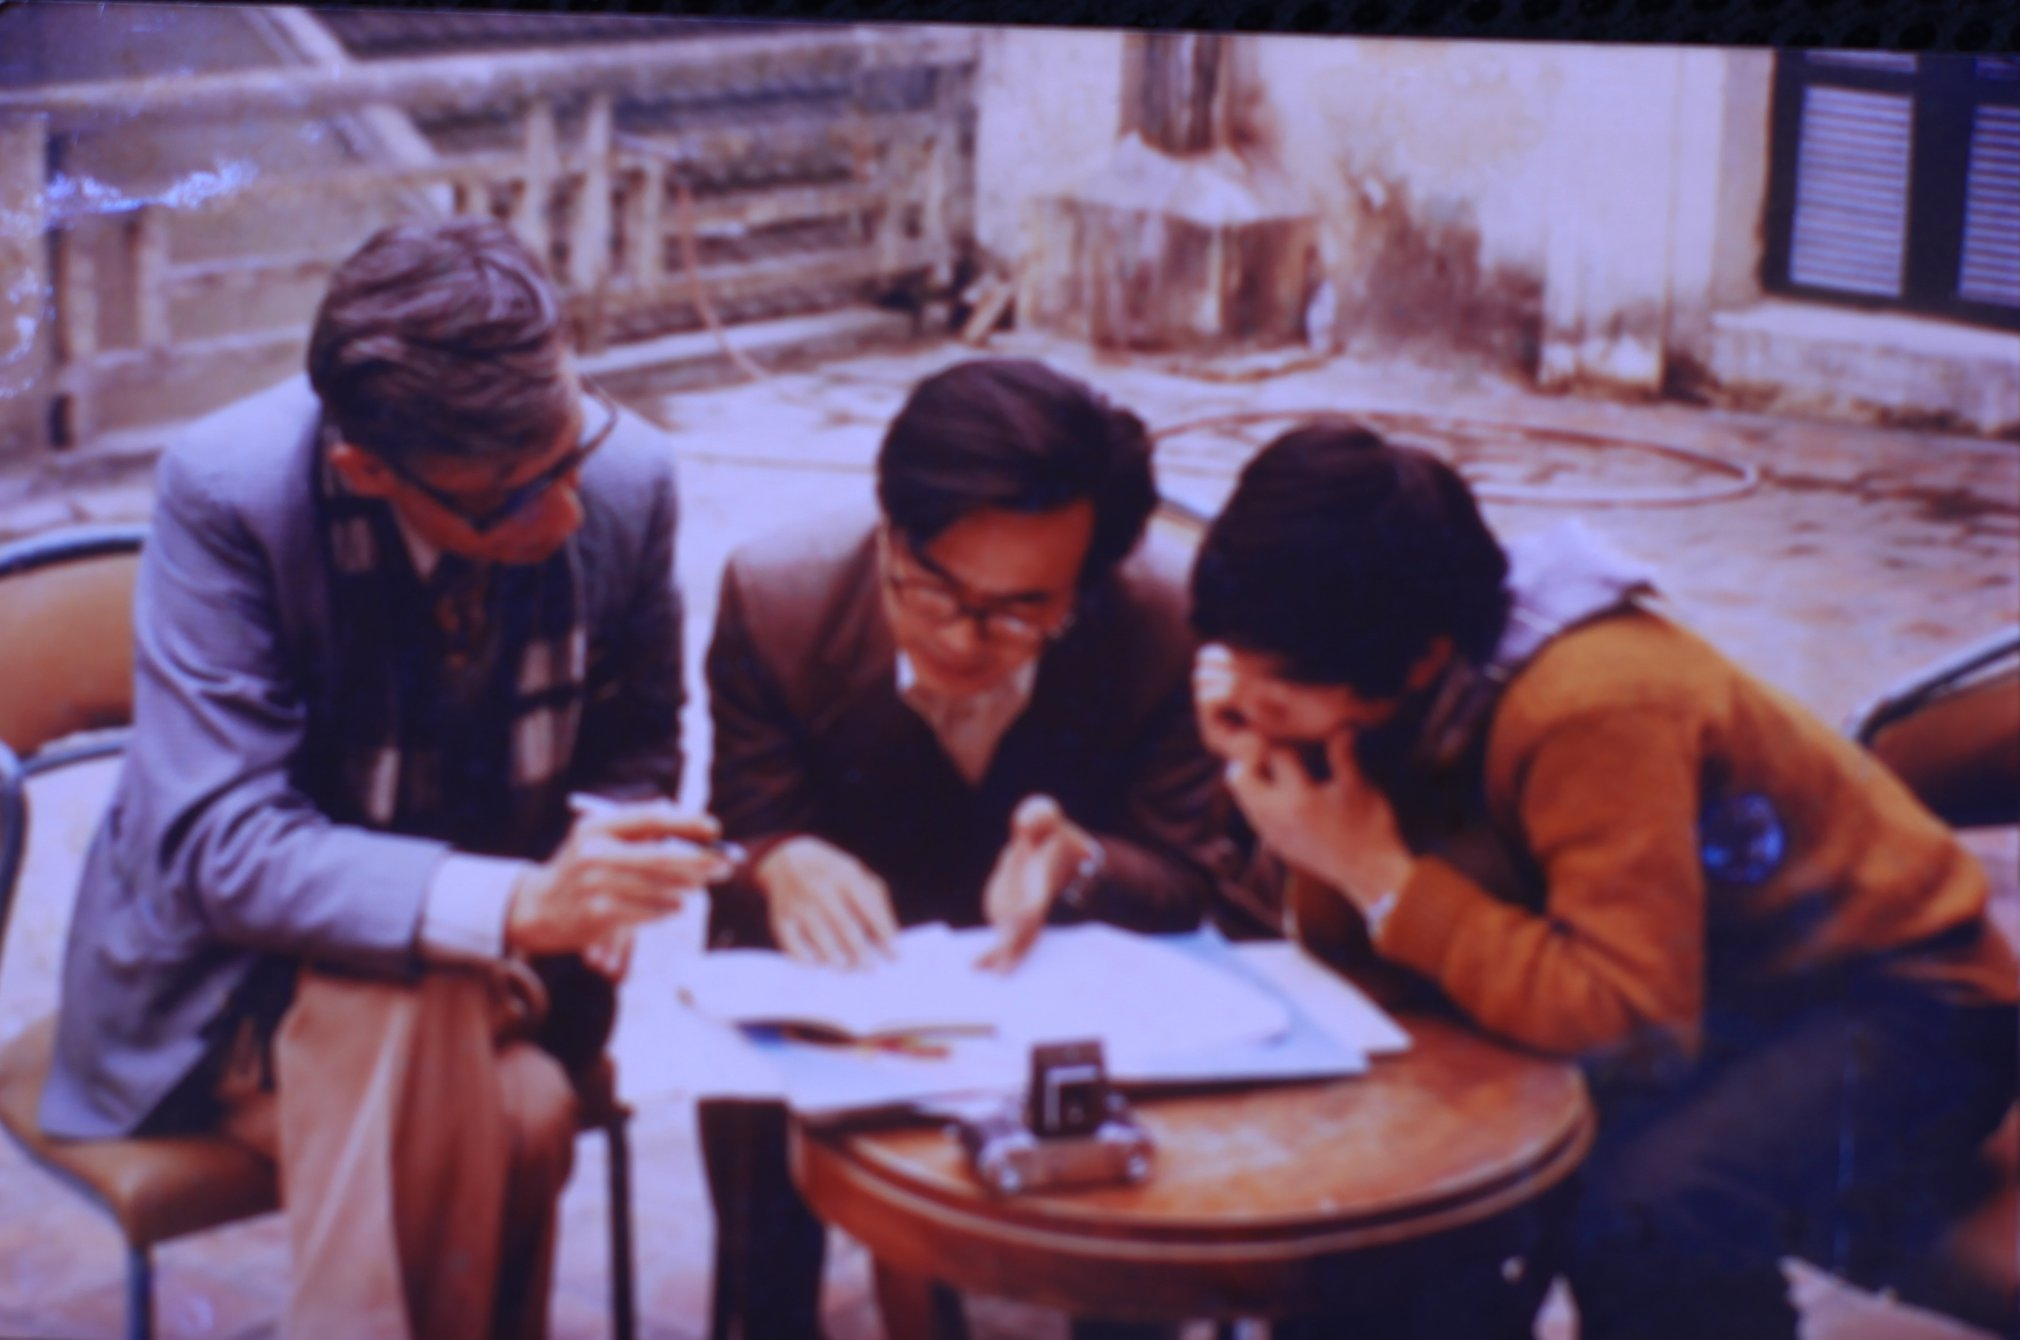
\includegraphics[scale=0.1]{Photos/NguyenChiCong}
\caption{Cuối tháng 2-1979, ngay sau sự kiện TQ xâm lược, tôi tiếp tục đươc tham gia cùng GS H.V. Regemorter và P.Đ. Diệu chuẩn bị kế hoạch đưa ace VN sang Pháp thực tập. Photo (c) CCSTV 1979 tại KS Hoàn Kiếm}
\end{figure}

VÌ SAO MẤT NGỦ

Anh ra đi vào sáng Chúa Nhật hay ngày Thái Dương, và buổi tiễn đưa Anh cuối cùng đã được gia đình thông báo chính thức sẽ tổ chức vào sáng thứ Sáu tức 18-5-2018.

Theo kế hoạch của nhóm Cyclo, lẽ ra chúng tôi phải kết thúc một công việc chung và giao nộp kết quả vào ngày mai 17-5. Nhưng đến phút này, riêng tôi cần xin lỗi các đồng nghiệp vì vẫn chưa thể tập trung suy nghĩ và chỉ đẻ ra ít trang chữ lộn xộn. Cũng trong tâm trạng ngơ ngẩn và sức khoẻ sút kém, tôi đã không thể đến dự buổi giới thiệu cuốn sách tái xuất bản Cái trống thiếc do nhà văn Dương Tường chuyển ngữ.

3h sáng. Không ngủ được, phải ngồi dậy uống trà gừng chống tụt huyết áp. Ngẫm lại mấy ngày qua dù sao cũng đã làm được hai việc có ích để từ giờ có thể cầm bút viết về Anh mà không còn lo sợ quên những điều cần đến tính xác thực. Thứ nhất là tìm ra không ít tư liệu về Anh, thứ hai là cho đăng lại một bài viết của Anh với nhan đề
\href{http://dongtac.hncity.org/?Hai-niem-hanh-phuc-gan-bo-voi-tin-hoc}{Hai niềm hạnh phúc gắn bó với tin học}.

Sau khi lần lượt tìm lại được cả hai chiếc điện thoại: một chiếc để quên trên xe khách và một chiếc bị văng ra do va chạm giao thông, tôi đọc FB và thấy cần nói vài điều với tư cách là một cộng sự rất gần gũi của Anh từ năm 1973 cho mãi đến khi nghỉ hưu. Trước đây vào năm 2007, nhân dịp kỷ niệm 30 năm thành lập Viện Khoa học Tính toán và Điều khiển, theo lời đề nghị của tạp chí Tin học và Đời sống, tôi có viết một hồi ức liên quan đến tập thể các kỹ sư trẻ và Viện trưởng là Anh, một TSKH lúc đó chưa được phong học hàm giáo sư. Toà soạn đã cho đăng liên tiếp ba kỳ, bạn đọc có thể tham khảo ở đây:

Kỳ 1: Chiếc máy vi tính đầu tiên của Việt Nam

Kỳ 2: CÁC THIẾT KẾ MỚI

Kỳ 3: SẢN XUẤT VÀ ỨNG DỤNG

Sinh thời xung quanh Anh, một con người với cuộc đời cực kỳ phong phú, đã từng có biết bao lời bàn tán trái chiều như thói đời vẫn thế. Rồi nay không có Anh đối chất nữa thì càng tăng thêm hiện tượng nói theo cảm tính, đáng tiếc có không ít lời tưởng là tôn vinh mà thực ra làm linh hồn Anh không vui, bởi vì sự chính xác và trung thực vốn là điều Anh quý trọng như bản chất của những trí thức khoa học.

Tối hôm thứ Hai, tôi mở các album trong thư viện nhỏ và thấy ngay hình Anh, nhưng số lượng ít và nội dung có vẻ quan phương, không nói lên những giây phút đời thường của Anh và chúng tôi. Vậy là phải lê đôi chân phù thũng như đeo đá leo lên tận tầng tư để bê xuống mhững túi nhỏ, cứ thế trong ba buổi mất chục lần lên xuống mới tạm yên lòng.

Tôi đã lục tung từng quyển sách trong thư viện lớn rồi lại sang kho mở hết tất cả những thùng giấy phủ đầy bụi bặm. Kết quả là ho rũ rượi và dị ứng toàn thân. Nhưng sau vài lần leo lên leo xuống thì cuối cùng cũng đã hòm hòm tập hợp được vài trăm tấm ảnh cũ kỹ. Ngay tối hôm qua tôi bắt đầu chọn lọc từ đó ra những bức có hình của Anh và gia đình Anh.

Nguyễn Chí Công


\chapter{Vĩnh biệt Giáo Sư Phan Đình Diệu (Đào Kiến Quốc)}

Vừa đọc trên Fb của GS Trần Văn Nhung và được biết GS Phan Đình Diệu đã mất. 

Tôi tốt nghiệp đại học toán Đại học Tổng hợp năm 1976 và được chọn ở lại trường làm giảng viên, nhưng được yêu cầu chuyển sang ngành Máy tính điện tử. Thời gian học máy tính ở khoa Toán, tôi chỉ biết một chút về lập trình và nguyên lý máy tính. 

Theo quy định thời đó, cán bộ giảng dạy phải tập sự hai năm và phải thi 4 chuyên đề. Ngành này khá mới mẻ, lúc đó ở bộ môn toán học tính toán chưa có ai là TS ngành máy tính (lúc đó gọi là chuyên ngành đảm bảo toán học cho máy tính) ngoài thầy Nguyễn Bá Hào thì lúc đó đã chuyển đi nơi khác . Chủ nhiệm Khoa (thày Hạp) mới gọi tôi lên đưa cho tôi một cái thư tay bảo: "Em sang bên Viện khoa học Tính toán và Điều khiển gặp thày Diệu, đây là thư tôi nhờ thày hướng dẫn cho em trong thời gian tập sự". 

Lúc bấy giờ Viện khoa học tính toán và điều khiển mới được thành lập, đóng đô ở Đồi Thông. Cứ sáng thứ 7 ở đó có xemina. Hầu hết những hành trang ban đầu về tin học tôi có là từ những xê mi na này. Thày Diệu hỏi han một chút và bảo: " Mình không có nhiều thì giờ lắm, Quốc đọc những cuốn sách này và thi với mình". Cuốn sách ông đưa là cuốn Ngôn ngữ hình thức và Chương trình dịch.   Hôm thi cũng thi trong lúc đang xê mina. Ông viết sẵn đề lên một nửa tờ A4 và tôi làm bài thi trong khi mọi người xê mi na. Tôi thi với thày Diệu 2 chuyên đề, còn hai chuyên đề khác thi với thày ở trong khoa.

Ông là người cực kỳ uyên bác và khúc triết. Nhưng bài ông trình bày trong xemina đều rất sâu sắc. Thời làm TS Khoa học bên Nga, thày làm về toán học kiến thiết, một thứ toán có liên quan mật thiết đến lý thuyết tính toán. Toán học kiến thiết không thừa nhận luật phản chứng, không thừa nhận vô hạn tiềm năng, chỉ thừa nhận vô hạn thực tai, không thừa nhận sự tồn tai theo kiểu kinh điển mà tồn tại tức là phải có một quy trình chỉ ra được sau hữu hạn bước. Điều này thật phù hợp với tư duy máy tính. Nghe nói, khi thành lập Viện Khoa học Tính toán và Điều khiển, người ta giao cho TSKH Nguyễn Thúc Loan làm Viện trưởng và chính ông Loan sau một thời gian ở vị trí này đã nói, xin để anh Diệu làm Viện trưởng, anh ấy làm sẽ tốt hơn tôi.

Thày xứng đáng được coi là người khai sinh ra ngành Tin học của Việt Nam. Thời đó tại Đồi Thông, VN là nước Đông Nam Á đầu tiên chế tạo ra máy vi tính theo đúng nghĩa. Rất nhiều các chuyên gia đầu ngành Tin học được đào tạo ở đây và ở Pháp qua đường hợp tác giữa VN và Pháp do Viện chủ trì.

Sau này do có sự bất đồng với lãnh đạo Viện hàn lâm KHVN, thày Diệu chuyển về làm cho Chương trình Quốc gia về CNTT giai đoạn 1996-2000 (thường được gọi là IT2000). Chương trình này đã đặt ra những nền tảng cho sự phát triển CNTT của VN sau này trong đó có việc thành lập các khoa CNTT trọng điểm, việc xây dựng các CSDL quốc gia, việc tin học hóa hành chính nhà nước. Năm kia tôi đọc lại các tài liệu về chương trình này và vẫn không hết ngạc nhiên về tầm nhìn của GS mặc dù đã qua 20 năm. 

Sau này ông xin về Đại học Quốc gia, Ông muốn tiếp tục cống hiến trong lĩnh vực giảng dạy. ĐHQG muốn ông về làm việc trực tiếp ở Khoa CNTT nhưng khoa tôi lại muốn ông sinh hoạt ở ĐHQGHN và chỉ giảng dạy ở Khoa, Khoa có một phòng làm việc dành riêng cho ông. Tôi có hỏi một lãnh đạo Khoa khi đó rằng tại sao lại đối xử như vậy thì được trả lời (chẳng hiểu có thật không) rằng "Tầm cỡ ông Diệu là phải có người giúp việc, có xe đưa xe đón thì khoa mình lo sao được", sau lại nói nhỏ  "phức tạp lắm đấy, mày có biết ai quan hệ với ông Diệu đều bị để ý không?"

Thời đó thày Diệu rất nổi tiếng theo kiểu một nhân vật bất đồng chính kiến khi ông từng nói về Lê Duẩn, "Ông Lê Duẩn là người rất vĩ đại, đã từng lãnh đạo Việt Nam đánh thắng Mỹ, thống nhất đất nước, nhưng sẽ vĩ đại hơn nếu từ chức TBT". Là đại biểu quốc hội, Ông có một lần đọc tham luận tại Quốc hội, một bản tham luận có tính phản biện cao, gây tiếng vang lớn mà thoát được sự kiểm duyệt trước. Ông luôn là người trăn trở với đất nước.

Sau khi bị đột quỵ, ông ít khi xuất hiện. Bức ảnh dưới đây là bức ảnh cuối cùng tôi chụp với ông trong buổi kỷ niệm 25 năm ngày thành lập Hội Tin học Việt Nam mà ông là Chủ tịch đầu tiên. Hồi đó ông đã yếu, đi lại chị Hương  phải dìu nhưng ông vẫn minh mẫn. 

Lần cùng với một số cán bộ khoa CNTT đến khoa cấp cứu A9 của bệnh viện Bạch Mai thăm ông, tôi phải đứng ngoài không nhìn thấy ông, nghe nói ông đang thiếp đi, tôi chỉ nói chuyện được một chút với con trai ông đang ở bệnh viện trông bố.

Xin chúc GS Phan Đình Diệu an nghỉ trong sự quý trọng và biết ơn của cộng đồng những người làm Công nghệ Thông tin. 
Vĩnh biệt giáo sư, 
Xin gửi lời chia buồn sâu sắc tới gia đình GS.

\chapter{Vĩnh biệt người anh cả ngành Công Nghệ Thông Tin (Nguyễn Công Hoá)}

Lúc 10h sáng 13/5/2018 GS. TSKH Phan Đình Diệu đã thanh thản về an nghỉ nơi Vĩnh hằng hưởng thọ 82 tuổi. Xin gửi lời chia buồn sâu sắc  đến toàn thể gia quyến của Giáo sư.

Đã nhiều báo có bài viết về nhà Khoa học lớn của đất nước trong lĩnh vực Toán học, Triết học...Phan Đình Diệu.Tôi nhớ về GS Phan Đình Diệu như Người anh cả của ngành Công nghệ thông tin (CNTT) và khoa học tính toán của nước nhà. Ngày hôm nay chúng ta được hưởng những thành quả ứng dụng CNTT và Internet ở Việt Nam là có sự góp sức từ thuở ban đầu không nhỏ của anh khi triển khai Nghị Quyết 49/CP “ về phát triển Công nghệ thông tin của nước ta trong những năm 90” do Thủ tướng Võ Văn Kiệt ký ban hành ngày 4/8/1993. Anh cũng là Phó trưởng ban chuyên trách, Thường trực Ban chỉ đạo Chương trình Quốc gia đầu tiên của Việt Nam ( 1994-1998). 

Anh chính là người sáng lập và là Chủ tịch đầu tiên của Hội Tin học Việt Nam ( 1988) là Viện trưởng đầu tiên cuả Viện Khoa học Tính toán và Điều khiển, nay là Viện Công nghệ Thông tin ( 1977).

Vĩnh biệt người Thủ trưởng, người Thầy và  người Anh đã  làm việc cùng tôi, dìu dắt tôi từ tuổi thanh niên đến suốt 20 năm (1977-1997). Kính chúc hương hồn anh an giấc ngàn thu trên cõi Niết Bàn. Mong anh luôn phù hộ cho sự nghiệp phát triển CNTT của nước nhà vượt qua mọi thăng trầm để sánh ngang với bạn bè Năm Châu. 

% Kính tặng Anh 4 câu Thơ như một lời tri ân:

% TIẾC THƯƠNG ANH

% Bầu trời lại tắt một ngôi sao

% Bạn hữu xa anh nước mắt trào

% Trí tuệ uyên thâm đời bác học

% Đức tài trọn vẹn sống thanh cao

% -------------

%Chú gửi cháu 2 bài Thơ Đường luật trọn dạng “ Thất ngôn bát cú”
%kính tặng hương hồn Bố cháu. Sinh thời bố cháu là một người rất uyên bác về Thơ Đường đấy. 
Hai bài Thơ kính tặng hương hồn  người Thầy, người Anh Phan Đình Diệu:

TIẾC THƯƠNG ANH

Bầu trời lại khuyết một ngôi sao

Bạn hữu xa anh nước mắt trào

Trí tuệ uyên thâm đời bác học

Đức tài trọn vẹn sống thanh cao

Lo về quốc pháp lời trang trọng

Nghĩ tới gia phong nét tự hào

Khí phách sĩ phu Nhân Nghĩa Dũng

Vui cùng thơ phú thú tiêu dao

(15/5/2018)

VĨNH BIỆT ANH 

Tiễn biệt anh rồi dạ ngẩn ngơ

Bồng lai Tiên cảnh đón vô bờ

Nơi kia Anh nghỉ ngàn thu mộng

Cõi ấy Anh nằm vạn giấc mơ

Quốc sách thông tin còn để lại

Lời khuyên Giáo dục vẫn đang chờ

Thiên Đường dạo ngắm hồn thanh thản

Vẹn nghĩa chung tình đẹp ý Thơ

(18/5/2018)

/Nguyễn Công Hoá/


\chapter{Vài kỷ niệm với Giáo sư Phan Đình Diệu  (Hiệu Minh)}

Nguồn: \href{http://meddom.org/vai-ky-niem-voi-giao-su-phan-dinh-dieu-gudi/}{Hiệu Minh}

Viện KHVN có hai anh tên vần “iêu”: Viện sỹ Nguyễn Văn Hiệu và Giáo sư Phan Đình Diệu. Một anh là viện trưởng, anh kia là viện phó, cùng giỏi và nổi tiếng khắp thế giới.

Cả hai đã về hưu. Một người huân huy chương đầy ngực, người kia chẳng có cái nào. Nhưng không vì thế mà kém cạnh nhau.


Anh Diệu có con trai là Phan Dương Hiệu. Dân hàn lâm đồn thổi, anh Diệu ghét anh Hiệu, đặt tên con để chửi cho sướng. Thật ra, Dương Hiệu nói ngược là Diệu Hương, tên của anh Diệu và chị vợ là Hương ghép lại, chả liên quan gì đến bác Hiệu.

Ai từng làm việc với anh Hiệu thì phục cũng có mà chê cũng lắm, thậm chí còn gọi đùa là Hiêu, vì hứa mà không làm.

Quân của anh Diệu thì tâm phục, khẩu phục tới 90\%, 10\% còn lại là do tỵ hiềm, ghen ghét, hoặc do lề phải trái. Chưa ai dám gọi anh là Điêu mà dân biết tiếng Pháp gọi anh là Monsieur Dieu – anh Trời.

\begin{center}
\textbf{Nhiệt huyết với khoa học}
\end{center}

Nói về đóng góp của Giáo sư Phan Đình Diệu cho khoa học nước nhà thì báo chí viết chán rồi. Tốt nghiệp tiến sỹ toán lý ở tuổi 30 vào cuối năm 1960 tại Liên Xô, thời đó là ghê răng.

Anh có công lớn trong việc tạo ra ngành Tin học Việt Nam, định hướng phát triển trong nhiều năm. Mình từng nghe các seminar về automat hữu hạn, ngôn ngữ hình thức, lý thuyết mật mã, triết học và toán, hội trường đông nghịt.

Tổng Cua từng viết những chương trình dựa vào thuật toán bảo mật của Giáo sư bằng Pascal vài ngàn lệnh cùng với Vũ Đình Hòa và mấy tay chuyên toán cự phách khác. Anh nói về khóa bảo mật cực phức tạp còn dễ hơn các bạn viết còm. Anh bảo, cái đẹp Toán học nằm ở sự đơn giản và logic. Mình viết blog được là học bài của anh Diệu.

Là người có tâm với khoa học và rất yêu toán và tin, anh bỏ không biết bao công sức để xây dựng ngành này cho nước nhà cùng với những giáo sư đầu ngành như Tạ Quang Bửu, Hoàng  Tụy, Lê Văn Thiêm, Nguyễn Văn Đạo…

Đi sang Pháp, thay vì dành tiền mua xe Peugeot về bán lấy lãi như nhiều người, anh mua rất nhiều linh kiện PC cho Viện. Đến nỗi đám quân thương quá, bảo anh đưa tiền, thay vì mua chip, mấy cha láu cá mua một cái xe gửi cho chị Huơng. Làm khoa học cũng phải có “động cơ”, các lão nói vậy.

Nhớ có lần mưa lụt hầm chứa máy tính ODRA, giáo sư đến thấy thảm cảnh đó mà rơi nước mắt vì biết bao tiền của mới mua được cái máy duy nhất thời đó ở miền Bắc.

Giáo sư nổi tiếng vì những quan điểm chính trị đổi mới vì anh nghiên cứu triết học và toán rất kỹ, hiểu rõ qui luật phát triển. Rất nhiều báo cáo của Đại hội Đảng liên quan đến KHKT thường do anh chấp bút. Tuy vậy, nhiều lời cố vấn quan trọng của người trí thức cũng chỉ dừng trên giá sách.

\begin{center}
\textbf{Những dự đoán tương lai}
\end{center}

Tổng Cua nhớ một số dự đoán tầm quốc gia và cả quốc tế của anh Diệu mà sau đó đã đúng.

Thấy Viện sỹ Nguyễn Văn Hiệu bổ nhiệm cán bộ lung tung, rồi biến viện KH VN thành những công ty nhỏ, Giáo sư đoán, cung cách này sẽ đưa viện khoa học đến sự tàn lụi. Quả thật, “nhân bảo như thần bảo”.

Đọc đề án 112 (tin học hóa quốc gia) năm 2001 có nhiều điểm bất bình thường, anh dự báo, dự án sẽ thất bại và gửi thư khẩn cho Thủ tướng Phan Văn Khải. Quả thật sau 5 năm, ban quản lý ra tòa và hàng nghìn tỷ mất mát.

Có lần đi công tác bên Bulgaria (1986), anh Diệu mang theo cháu Phan Dương Hiệu và bà xã Văn Thị Xuân Hương, em gái của giáo sư Văn Như Cương, toàn vần ương.

Anh kể chuyện năm 1954, tốt nghiệp trung học ở Hà Tĩnh rồi đi bộ ra Hà Nội để học trường ĐH Khoa học. Anh nói là gien của anh là làm toán, không phải để làm quan. Nhưng cuối cùng người ta cứ nhét chức cho anh, khổ thế.

Cuối những năm 1970, cấp trên thấy Giáo sư trẻ và rất giỏi, đề nghị đưa anh vào Đảng để làm cán bộ nguồn, dù khi đó đã làm Viện phó Viện KHVN.

Chị Hương, đảng ủy viên, có trách nhiệm phát triển đảng cho chồng. Tỷ tê về tương lai, rồi lợi ích nếu là người của Đảng thì như thế nào, và khuyên, anh chỉ cần viết đơn là họ kết nạp ngay.

Anh nói, để nghĩ 10 ngày rồi trả lời. Đúng hẹn, anh bảo, Đảng muốn thì cứ kết nạp, cần gì phải viết đơn. Thế là chuyện vào Đảng xếp lại. Quan lộ cũng vì thế mà chẳng hanh thông. Ngang ngạnh kiểu ông đồ xứ Nghệ quả có một không hai.

Nhớ lần đi thang máy lên đỉnh Vitusha của thủ đô Sofia đầy tuyết trắng, thay vì mơ mộng với trời mây, bỗng anh than, với cung cách quản lý của các nước XNCH, thế nào khối này cũng sụp đổ cho mà xem. Lúc đó, Tổng Cua nghe rất choáng, và thấy Giáo sư hơi… phản động.

Anh kể, đã sang Hungaria, CHDC Đức, Ba Lan, Tiệp Khắc, Liên Xô, Mỹ và Tây Âu, nhận xét thế là có lý riêng của mình.

Ba năm sau, bức tường Berlin sụp đổ (1989), kéo theo toàn bộ Đông Âu và Liên Xô tan rã.

Anh là đại biểu Quốc hội lúc hơn 40 tuổi, một trong đại biểu trẻ nhất thời đó. Trong một lần được hỏi về một vị quan cao nhất và ảnh hưởng của ông đối với đất nước, anh Diệu có nói đại ý, vị lãnh đạo ấy rất vĩ đại, đưa cuộc kháng chiến chống Mỹ tới thắng lợi, nhưng vĩ đại hơn, nếu ông từ chức ngay bây giờ.

Lúc đó, vị lãnh đạo kia đang ở thế thượng phong sau 1975 chiến thắng vang dội. Nhưng rồi chính sách tập thể HTX, hợp tỉnh, giá lương tiền quá kém cỏi trong thời bình đã đẩy đất nước đến thảm họa. Người dân chỉ mong ông ấy ra đi.

Mang triết lý chiến tranh vào xây dựng thời bình là không thể, mỗi người có một thời. Anh Diệu từng từ quan về làm nghiên cứu khoa học, góp ý phát triển đất nước theo quan điểm của thời đại mới, cho dù những lời của Giáo sư rất khó nghe đối với nhiều chính trị gia.

Thật tiếc, những đầu óc có tầm vóc quốc tế như Giáo sư Diệu mà ít được sử dụng đúng mục đích. Nước mình quá lãng phí chất xám.

\begin{center}
\textbf{Viện trưởng giỏi việc “nước”, đảm việc nhà}
\end{center}

Viện IOIT có mấy cái nhà ngói hình chữ U. Mỗi lần trời mưa, ếch nhái kêu râm ran. Mình thì tối ngủ bàn cơ quan, ăn cơm tập thể chợ  Ngọc Hà. Gia tài là cái xe đạp Wilga mầu đỏ của Ba Lan, đi vài năm đã hỏng. Quần áo rách dần, tích kê mông, đầu gối, áo sờn. Lốp xe vá chằng vá đụp.

Mặt mũi vêu vao như kẻ chết đói. Đang tuổi ăn tuổi ngủ mà có 13kg gạo/tháng, lương 51 đồng. Mỗi lần về quê, mẹ phải cho thêm vài cân gạo cứu đói vào chiếc ruột tượng, gói cho mấy quả trứng và chai mắm tép. Bố thở dài, kỹ sư chó gì mà nghèo rớt mồng tơi. Hay là về đi cày, ăn no hơn. Học cho lắm chữ mà chẳng nên cơm cháo gì.

Thời đó ai cũng thế. Giáo sư Diệu cũng chẳng hơn gì. Phòng Viện trưởng khoảng $8m^2$, đủ kê cái bàn, 4 cái ghế mây, bàn uống nước, sàn lát gạch thô, trần cót ép, không điều hòa, có cái quạt máy điện cơ chạy lừ đừ như ốm đói.

Nhưng đám trẻ cũng vui vì có em Ngân chân dài, xinh đẹp làm thư ký, đi lại phấp phới. Em Thoa má bánh đúc, trông mỡ màng, làm thư viện. Em Liên cá vàng xinh như mộng, đục lỗ bìa máy tính ODRA.

Các viện sỹ trẻ thi nhau đong đưa, gọi viện là Tán tỉnh và Tiêu khiển cũng không ngoa. Anh cũng thông cảm và bảo, đàn ông thấy người đẹp mà không ngắm thì hoặc anh ta nói dối hoặc là bị bệnh.

Anh Diệu ở tầng 5 bên khu lắp ghép Giảng Võ, vì làm quan được lên tầng cao sạch sẽ và mát. Chỉ tội không có nước. Sáng sáng, trước khi đi làm, Giáo sư cởi trần, xách nước từ tầng một lên tầng năm. Thời đó, ban ngày cả nước lo việc nhà, ban đêm cả nhà lo việc nước, Viện trưởng IOIT cũng vậy thôi.

Khi được cấp nhà rộng hơn ở Đồng Xa, mấy phòng liền, cả gia đình chuyển về đó. Thực không ngờ, nơi đó đồng không mông quạnh, chỉ có đồng lúa, ếch nhái kêu, cào cào châu chấu, thiêu thân và bướm đêm bay rợp trời. Điện mất, nước mất, khổ đủ điều. Viện trưởng tiếp tục thức đêm xếp hàng nước và giặt tã.

Là quân của anh ấy mà Tổng Cua chẳng bao giờ biếu xén thủ trưởng. Trong khi mình sang chơi là chị Hương mời vồn vã, chú ở lại ăn cơm, độc thân trông đói hom hem, khổ thân chú. Thủ trưởng hối lộ quân, chuyện ngược đời.

\begin{center}
\textbf{Nghiên cứu bỏ thuốc lá…ra con trai}
\end{center}

Cái nghề nghiên cứu khoa học nước mình hay lắm. Nghiên cứu một đằng, kết quả ra một nẻo. Giáo sư Diệu nghiên cứu cai thuốc lá thì vợ đẻ con trai.

Chả là Giáo sư có hai cô con gái là Quỳnh Dương và Hà Dương đều rất xinh và hiền. Như nhiều nhà, hình như anh mong có con trai.

% \begin{center}
% 
\includegraphics[scale=0.5]{ntngochai_phandinhdieu}\\
%  Hai ông bà Hương-Diệu. Ảnh: Ngọc Hải
% \end{center}

Anh Diệu nghiện thuốc lá nặng, phòng làm việc lúc nào cũng nghi nghút như cái lò gạch của Nam Cao. Ai đi công tác về cũng biếu thuốc lá, từ 555 đến Pall Mall, Malborro, Tam Đảo, Điện Biên, đủ loại tây ta.

Vợ khuyên bỏ thuốc mãi không được nên ra giá, anh bỏ được, em sẽ đẻ con trai. Giáo sư hứa đại. Thật bất ngờ, cuối năm ấy, cháu trai Phan Dương Hiệu ra đời. Thế là đành phải thực hiện lời hứa. 

Mấy ngày đầu Giáo sư không chịu nổi, cứ cầm điếu thuốc lên, hút vài hơi rồi dụi tắt. Dần dần anh mang các bao thuốc bóc sẵn để khắp nơi trong nhà, trên giá sách, chỗ bàn ăn, văn phòng, nơi hay sờ tới nhất. Nhìn thấy thuốc nhưng không cầm.

Sau ba tuần anh cai hẳn. Vợ đùa dù hơi lo “Anh Diệu bỏ được thuốc nghĩa là anh ấy có thể bỏ vợ được”.

\begin{center}
\textbf{Sửa gáy Giáo sư được trả công bằng…việc làm}
\end{center}
Năm 1977, anh Diệu, lúc đó khoảng 40 tuổi, Viện trưởng Viện Tính toán và Điều khiển đi thăm các nước XHCN và tìm nhân tài cho viện.

Anh tới Ba Lan vào mùa xuân , tuyết vẫn còn dầy. Gần 200 lưu học sinh VN đón giáo sư trẻ ở ký túc xá trên đường $\dot{Z}wirki i Wigury$, đại lộ huyết mạch từ sân bay $Warszawa-Okecie$ về trung tâm Thủ đô Ba Lan.

Bác đoàn trưởng tên là Loan, giám đốc Nha khí tượng Thủy văn đang làm NCS, gõ cửa phòng và bảo “Anh Cua sang nhờ tý”. Mình sang thì gặp Giáo sư Diệu rất trẻ và dễ mến. Anh cười và bảo “Nghe nói cậu biết cắt tóc, chiều nay tớ có cuộc nói chuyện, đi nhiều nước mà không có thời gian. Cậu giúp tớ nhé”.

Giọng Hà Tĩnh hơi nặng, anh xưng cậu cậu tớ tớ, nghe rất thân mật và không hề quan cách. Mới gặp đã thấy rất cảm tình. Trán rộng, mặt sáng, trông rõ là… bác học.

Thời đó sinh viên Ba Lan nổi tiếng tóc dài quần loe, hippi, sexy, thu thập ảnh các cô trần truồng, treo cả lịch 365 thế làm tình trong phòng, chỉ tội không có giáo cụ trực quan để thực hành. Cắt tóc chỉ là xén bớt phần dài dưới gáy.

Trong khi anh Diệu muốn có mái, rẽ ngôi. Loay hoay một hồi, mình cũng sửa xong cái gáy Giáo sư. Anh hỏi Cua “Cậu học nghề chi?”. Mình bảo là Toán Tin. Thế à, cậu về chỗ mình nhé.

Mình bảo, em học dốt lắm, không có bằng đỏ đen gì đâu, lại còn đúp nữa đó. Anh khuyên, tớ không cần bằng đỏ, mà lấy người về nghiên cứu khoa học, và làm được việc. Rồi anh giới thiệu viện, cho số điện thoại, địa chỉ.

Đang du học nên chả nghĩ đến xin việc vì hồi đó cho rằng làm đâu cũng là xây dựng CNXH. Khi về Hà Nội mới hiểu là cái bán kính 3km lấy tâm là bờ Hồ vô cùng quan trọng. Mình lên Nghĩa Đô tìm, không hy vọng anh nhớ mình là ai. Hóa ra Giáo sư nhớ cả tên.

Anh viết thư tay lên Bộ ĐH, thế là mình nghiễm nhiên thành viện sỹ, nằm bàn, cơm tập thể, ước mơ xây XHCN và tiến lên CNCS vào cuối thế kỷ 20.

\begin{center}
\textbf{Khử virus PC được vợ}
\end{center}

Nếu so sánh hai gia đình các anh vần “iệu” ở Viện KH Việt Nam, phải công nhận thuyết “nhân quả” rất đúng. Cha mẹ sống nhân nghĩa để đức cho con. Không biết anh Nguyễn Văn Hiệu thế nào chứ gia đình anh chị Diệu-Hương hạnh phúc, con cái thành đạt.

Con gái thứ là Phan Thị Hà Dương, từng giành được Huy chương Đồng Olympic Toán quốc tế năm 1990, Tiến sỹ Toán khi 26 tuổi và hiện đang công tác trong nước.


% \begin{figure}[!ht]
% \centering
% 
\includegraphics[scale=0.5]{haduong}
% \caption{Tiến sỹ toán Hà Dương }
% \end{figure}


Cháu Phan Dương Hiệu hồi đi Bulgaria mới 8 tuổi. Lần đi chơi mình bảo, cháu ghi nhật ký thì nên đếm số cột điện treo thang máy từ chân lên đỉnh Vitusha (Sofia) làm kỷ niệm. Có lẽ do gien toán của bố nên cháu thản nhiên, cần gì phải đếm, số cột đã đánh rồi, chỉ cần lên đỉnh và xem số cột cuối là bao nhiêu. Cháu Dương Hiệu hiện là Tiến sỹ Toán đang ở bên Pháp.

Con gái đầu lòng là Quỳnh Dương, đẹp hiền, đảm, ít nói, ngoan, học giỏi và an phận. Hồi ở Đồng Xa, có lần chị Hương nhờ lão Cua tìm thầy trẻ dạy đàn ghi ta cho cháu Quỳnh. Mình hứa lung tung rồi quên tiệt.

Chị Hương quay sang tìm kỹ sư sửa máy tính cho gia đình. Cu Thắng, viện IOIT, khá đẹp trai, có ria mép, thông minh, nhận đến sửa đĩa cứng, rồi cài virus vào, thỉnh thoảng máy lại treo. Mà PC không treo thì Quỳnh Dương cũng gọi anh Thắng đến xem lại cho chắc.

Sau vài tháng, mình hỏi chị Hương là thế nào rồi. Chị bảo chán lắm, tình hình là rất tình hình, lần nào về cũng thấy hai đứa ngồi đối diện nhau, chả thấy nói gì.

Năm ấy Quỳnh Dương sang Pháp du học. Anh chị thở dài, nông nỗi này thì em Quỳnh ế mất. Cả nhà ra sân bay tiễn con, vừa thương vừa nhớ. Cậu Thắng xin đi theo, nhỡ máy laptop của Quỳnh có hỏng gì chăng.

Lên sân bay Nội Bài bịn rịn chia tay. Bỗng anh Diệu thấy con gái cưng, vốn hiền lành, ôm chầm thằng cu chuyên cài virus, nắm tay, nhìn nhau đắm đuối chẳng biết trời đất nào nữa, rồi hôn môi một cái rất dài.

Giáo sư bỏ kính xuống, không thể tin vào mắt mình. Đời anh từng quản lý hàng ngàn cán bộ khoa học, đưa ra những triết lý phát triển cho quốc gia, báo cáo khoa học quốc tế được cả ngàn người thán phục. Rồi suýt bị “dính chưởng” vì chị Dương Thu Hương từng có bài viết đa nguyên của Giáo sư trong vali khi bị bắt ở sân bay. 

Ngay cả cái lý thuyết automat hữu hạn phải gió hay cái máy vi tính đầu tiên của Việt Nam được xuất xưởng, anh cũng không ngạc nhiên bằng nụ hôn giữa thanh thiên bạch nhật của cô con gái  dành cho cu Thắng bên phòng Kỹ thuật số.

Hai vợ chồng choáng váng và chợt hiểu thế nào là virus PC nhiễm sang người. Họ thầm gọi cu Thắng là Thang Dieu – Thằng  Con Trời cho xứng với Monsieur Dieu – Ông Trời Diệu.

Sau cái vụ nhiễm virus ấy, hai đứa có mấy con và hiện đang sống bên Pháp, rất hạnh phúc. Chả hiểu cu Thắng có dạy đàn ghi ta cho Quỳnh không.

Còn Tổng Cua đang làm gì, đố các bạn biết? Lão cố dạy hai thằng cu Hiệu – Minh cách cài virus vào máy tính và học thêm nghề cắt tóc.

HM. 1-2-2012





\chapter{GS Phan Đình Diệu: Nhà toán học Việt Nam đầu tiên đi du học ở Liên Xô (cũ)! (Trần Văn Nhung)}
Nguồn: \href{https://dantri.com.vn/giao-duc-huong-nghiep/vinh-biet-gs-phan-dinh-dieu-kinh-men-20180514225309113.htm}{Báo Dân Trí}

GS Phan Đình Diệu là nhà toán học Việt Nam đầu tiên đi du học ở Liên Xô (cũ) mà luận án TSKH được đăng thành một tuyển tập riêng của Viện Toán học mang tên V. A. Steklov của Viện Hàn lâm Khoa học Liên Xô.

GS Phan Đình Diệu, nhà toán học, khoa học máy tính của Việt Nam đã qua đời lúc 10h sáng 13/5, sau một thời gian lâm bệnh. Lễ viếng GS Phan Đình Diệu bắt đầu từ 9h30 ngày 18/5/2018, tại Nhà Tang lễ Bệnh viện TWQĐ 108, số 5 Trần Thánh Tông, Hà Nội; Lễ Truy điệu vào hồi 10h30.

Linh tính lạ kỳ: Trưa chủ Nhật ngày 13/5/2018, khi đang đọc và chỉnh sửa lại bài viết cũ của mình về GS Phan Đình Diệu, tôi nhận được tin buồn: GS Phan Đình Diệu đã từ trần vào sáng hôm đó tại Hà Nội, hưởng thọ 83 tuổi.

GS TSKH Phan Đình Diệu (12/6/1936 - 13/5/2018, quê quán Can Lộc, Hà Tĩnh) là nhà toán học, nhà khoa học máy tính của Việt Nam, người có nhiều đóng góp quan trọng xây dựng nền khoa học, giáo dục, văn hóa nước nhà .

Ông là một trong những người được ghi nhận có công đầu trong việc đào tạo và phát triển ngành tin học Việt Nam, là chuyên gia trong các lĩnh vực: Toán học kiến thiết, logic toán, lý thuyết thuật toán, ôtômat và ngôn ngữ hình thức, lý thuyết mật mã và an toàn thông tin...



GS Diệu là viện trưởng đầu tiên của Viện Khoa học Tính toán và Điều khiển (nay là Viện Công nghệ Thông tin Việt Nam), Chủ tịch sáng lập Hội Tin học Việt Nam, phó Trưởng ban thường trực Ban chỉ đạo Chương trình Quốc gia về Công nghệ Thông tin khóa I (1993-1997), ...

Trên trang cá nhân của GS Phan Dương Hiệu (con trai GS Phan Đình Diệu) ngày 27/6/2017, thông báo đã mua được trên trang sách của Hội Toán học Mỹ cuốn sách in công trình khoa học của GS Phan Đình Diệu mang tên: "Some Questions in Constructive Functional Analysis" (tạm dịch "Một số vấn đề về Giải tích hàm Kiến thiết"), được xuất bản trong "Proceedings of the Steklov Institute of Mathematics", 1974.

Khi mới ra trường làm cán bộ giảng dạy trẻ của Khoa Toán-Cơ-Tin học, trường ĐH Tổng hợp HN, tôi đã nghe tin về cuốn sách này và sau đó được nhìn thấy bản tiếng Nga trong Thư viện Khoa và Trường.

Tôi không hiểu gì mấy về nội dung cuốn sách nhưng, cũng như nhiều người khác, tôi rất trân trọng và khâm phục một thành tựu khoa học ở đỉnh cao.

Ngay lúc đó tôi cũng được biết GS Phan Đình Diệu là nhà toán học Việt Nam đầu tiên đi du học ở Liên Xô (cũ) mà luận án TSKH được đăng thành một tuyển tập riêng của Viện Toán học mang tên V. A. Steklov của Viện Hàn lâm KH Liên Xô. Tôi láng máng hiểu được rằng công trình này của GS Phan Đình Diệu là những kết quả mới mẻ, hệ thống và rất quan trọng về toán học kiến thiết.

Ngoài việc nghiên cứu và ứng dụng toán học, tin học và làm quản lý ra, GS Phan Đình Diệu còn dành nhiều thời gian cho giảng dạy, nói chuyện, viết báo về toán học, tin học, khoa học, triết học, văn hóa ...

Các hoạt động khoa học này góp phần làm cho ông nổi tiếng và được hâm mộ ở trong nước và quốc tế.

Tôi còn nhớ một bài viết rất hay của GS Phan Đình Diệu trên Tạp chí Toán học và Tuổi trẻ (số 56, tháng 10-11/1970) giới thiệu về Bài toán thứ 10 do David Hilbert đề xuất năm 1900 tại Paris.

Sau chặng đường dài 70 năm “chạy tiếp sức” của nhiều nhà toán học tài năng trên thế giới, người hoàn tất chặng đường cuối cùng năm 1970 là nhà toán học Nga 23 tuổi Iu. V. Matchiasevich (1974-), sinh viên của ĐH Tổng hợp Saint Petersburg (CHLB Nga).

Bài toán được phát biểu như sau: “Hãy chỉ ra một phương pháp mà nhờ nó, sau một số hữu hạn các phép toán có thể khẳng định rằng một phương trình Diophantine là có nghiệm nguyên hay không”.

Phương trình Diophantine là phương trình có dạng P(x, y,..., z) = 0 trong đó P (x, y,..., z) là một đa thức với hệ số nguyên của các ẩn x, y, ..., z và khi giải người ta chỉ tìm các nghiệm nguyên hoặc nghiệm nguyên không âm của nó. (Như thế phương trình Fermat chỉ là một phương trình Diophantine đặc biệt).

Tiếc thay, câu trả lời cho bài toán Hilbert số 10 lại ở dạng phủ định: Không tồn tại phương pháp chung để với mọi phương trình Diophantine cho trước, có thể khẳng định được rằng nó có nghiệm nguyên hay không.

Khi trân trọng công trình khoa học xuất sắc của GS Diệu, tôi cũng rất trân trọng tình cảm và đóng góp khoa học từ những người con của GS Phan Đình Diệu như: GS Phan Dương Hiệu, PGS Phan Thị Hà Dương, Phan Thị Quỳnh Dương.

Tôi đặc biệt quý trọng những người con, người cháu, những công dân biết trân trọng, sưu tập, gìn giữ và phát huy những di sản văn hóa, khoa học, nghệ thuật, ..., do cha ông, dân tộc mình để lại.

Đấy là những người con, người cháu, những công dân hiếu nghĩa và có văn hóa cao, biết uống nước nhớ nguồn.

Người ta thường nói: Đằng sau sự thành công của người đàn ông có bóng dáng một người phụ nữ.

Đối với GS TSKH Phan Đình Diệu, đó là phu nhân Văn Thị Xuân Hương thông minh, xinh đẹp và đảm đang, cả việc nước việc nhà.

Chị Hương là em gái của PGS Văn Như Cương, một nhà toán học, một thầy giáo toán và hiệu trưởng tài năng, độc đáo với bộ râu quý hiếm.

Hai đồng nghiệp và tôi đã dịch cuốn sách của A. D. Aczel từ tiếng Anh ra tiếng Việt "Câu chuyện hấp dẫn về Bài toán Fermat", NXBGDVN, Hà Nội-2000 (178 trang, đến nay đã được tái bản 6 lần).

GS Phan Đình Diệu là một trong những người đầu tiên tôi gửi tặng cuốn sách này. GS nói với tôi: "Cám ơn Nhung đã tặng mình cuốn sách về Định lý lớn Fermat! Khi cuốn sách vừa đến tay, mình đã đọc một mạch chừng 2-3 tiếng đồng hồ liên tục, từ trang đầu đến trang cuối. Cuốn sách hay quá”!

Vĩnh biệt Anh, GS TSKH Phan Đình Diệu kính mến!

GS.TSKH Trần Văn Nhung (14/5/2018)

\chapter{GS Diệu và những tiên tri chính trị chính xác (Nguyễn Đăng Hưng)}
\input{BaiViet/NguyenDangHung.tex}

\chapter{Vô cùng thương tiếc GS Phan Đình Diệu (Trần Văn Kinh)}

Mới có mấy tháng sau sự ra đi của PGS Văn Như Cương, mà như lúc sinh thời ông thường ví von, đó là sự “ánh xạ” của một phần tử  từ không gian này đến một không gian khác không “đẳng cấu”, giờ lại đến lượt GS Phan Đình Diệu ! Buồn biết bao nhiêu !

Cũng như Văn Như Cương và nhiều trí thức chân chính khác, hệ tư duy trong con người Phan Đình Diệu là hoàn toàn minh bạch. Từ đó, ông nhìn mọi hệ thống lành mạnh phải là hệ thống minh bạch, trong đó mỗi phần tử đều có chức năng rõ ràng và hệ thống được vận hành bằng những mối quan hệ cũng rõ ràng ! Mọi phần tử của hệ thống đó đều hiểu và hành động nhất quán và trung thực theo các chức năng và quan hệ đó. 
Không chấp nhận sự mập mờ khái niệm và sự “vận dụng” tuỳ tiện.
Ở đâu cũng thế và lúc nào cũng thế ! 

Ngành Toán học mà Phan Đình Diệu đã nghiên cứu và phát triển là Toán học kiến thiết. Nhà toán học tìm ra được điều gì mới thì phải chứng minh nó bằng cách chỉ ra được một quy trình (một thuật toán) để đi đến điều phát minh đó ! 
Phương pháp phản chứng ( tức là chỉ ra rằng nếu công nhận ngược lại thì sẽ đi đến mâu thuẫn), mặc nhiên thừa nhận luật bài trung ( loại trừ cái thứ ba ), chứ không hề dẫn dắt người ta đến điều cần chứng minh. 

Vì thế, mà Toán học kiến thiết không chấp nhận Phương pháp phản chứng ! Cũng tức là không công nhận Luật bài trung !
Tư tưởng đó mới mẻ biết chừng nào ! Và cần thiết biết chừng nào cho việc lập trình mà sự nở rộ và phát triển như vũ bão của nó đã dẫn đến quá trình tự động hoá, không phải chỉ trong vận hành cơ điện vật lý…mà cả trong và chủ yếu là trong hệ thống tự động hoá điều khiển, trong tư duy sáng tạo và trí tuệ nhân tạo !

Bây giờ, khi mà cuộc cách mạng 4.0 đang đến gần thì tư duy đó được công nhận là  sáng tạo và thực tiễn, nhưng 40, 50 năm trước, nó xa vời biết chừng nào, nhất là đối với những người mà tư duy đã dừng lại với “Đại công trường thủy nông”, với “Mo cơm, quả cà và tấm lòng cộng sản !”…
Nhưng xin đừng hiểu lầm rằng Toán học chỉ có ngành Toán học kiến thiết. Và cũng đừng hiểu lầm rằng nhà Toán học Phan Đình Diệu chỉ có nghiên cứu Toán học kiến thiết !
Ngay từ cuối những năm 60 của thế kỷ trước, tại Hội trường Uỷ ban Khoa học và kỹ thuật nhà nước ở 39 Trần Hưng Đạo Hà Nội, trong một chuỗi dài các Seminar dành cho các nhà Toán học của GS Tạ Quang Bửu như về “ Các cấu trúc của Bourbaki “ hay về “ Lý thuyết các Tai biến”… , nhiều buổi GS Tạ Quang Bửu và Giảng viên Phan Đình Diệu cùng nhau thuyết trình, hoặc có buổi chỉ mình Phan Đình Diệu thuyết trình, mặc dù lúc ấy ông chưa phải là Tiến sĩ, càng chưa phải Giáo sư !
Tôi cũng như nhiều bạn bè cùng lứa, may mắn được là bạn học cùng ông từ hồi phổ thông cho đến đại học, (cũng có cái không may là phải chịu đựng cái chủ nghĩa thành phần trong một giai đoạn, nhưng rồi cũng đã qua đi). Điều mấy mắn lớn lao của thế hệ chúng tôi là ở chỗ chúng tôi đã được hưởng thụ sự giáo dục từ những người thầy trí tuệ và tâm huyết mà những thế hệ sau không dễ gì có được ! 

Có thể nói hệ thống tư duy minh bạch, trung thực,  cùng với tài năng vượt trội của Phan Đình Diệu đã tạo nên uy tín lớn lao của ông trong lòng  bạn bè, đồng nghiệp, học trò, và nhiều người khác.

Còn nhớ ngày họp Đại hội thành lập Hội Tin học Việt Nam, tổ chức tại Cung Văn hoá Hữu nghị Việt Xô (nay là Cung Hữu nghị), ông được tín nhiệm gần như tuyệt đối, mặc dù mọi người cũng đều biết rằng bên cạnh ông , còn có nhiều nhà Tin học khác, cũng tài năng và tâm huyết !  Sau khi Ban Kiểm phiếu công bố kết quả bầu Chủ tịch Hội, cả Hội trường vỗ tay vang dội, rồi ùa lên sân khấu ôm nhau chúc mừng, và từ một góc nào đó trên sân khấu đã vang lên những bài hát nhạc chế Việt và Nga quen thuộc từ thời sinh viên….

Sau này, do công việc, tôi lại có dịp làm việc với ông trong vài trò là Uỷ viên thường trực của Chương trình Tin học hoá Quản lý ở Bộ Công nghiệp nhẹ (trước đây), trong khi ông là Phó Chủ nhiệm thường trực Ban chỉ đạo Chương trình Tin học hoá Quản lý của Nhà nước. Một lần tôi đã tâm sự với ông : “Tầm nhận thức của Diệu thì rất cao, mà thực tế thì đang rất thấp. Phải có nhiều người như bọn tớ nữa để có thể chuyển tải được điều Diệu mong muốn đến với thực tế !” Ông bảo ông không đồng ý như thế, nhưng ông đã nhiều lần cùng chúng tôi bàn cách đưa Tin học vào cuộc sống như thế nào. Những khái niệm như Tin học văn phòng, Tin học Tài chính Ngân hàng, Tin học Hàng không…ở nước ta dường như đã ra đời từ thực tiễn hoạt động ấy. Nhiều người có tài năng và tâm huyết đã đóng góp vào những thành công ấy, nhưng dấu ấn của Phan Đình Diệu là không hề nhỏ !
Bây giờ thì những dấu ấn ấy đã trở thành dĩ vãng xa vời ! 

Ước ao rằng Diệu sẽ gặp Cương và các bậc thầy đáng kính của chúng ta: các GS Tạ Quang Bửu, Lê Văn Thiêm, Trần Đại Nghĩa …tại một không gian “ánh xạ” nào đó !

Vô cùng thương nhớ Diệu !

Bạn cũ : Trần Văn Kinh


\chapter{GS Phan Đình Diệu: Một khối nghĩ suy đã đi xa...  (Chu Hảo)}
\input{BaiViet/ChuHao.tex}

\chapter{Theo dòng ký ức (Nguyễn Quý Dy )}

 
(TTĐN)-Người dân Can Lộc, Hà Tĩnh luôn tự hào về ``thần đồng'' toán học Phan Đình Diệu, một người con của quê hương. Năm 1965, khi mới 31 tuổi ông đã hoàn thành luận án tiến sĩ khoa học tại Đại học Tổng hợp quốc gia Moskva mang tên Lomonosov. Đối với những người nghiên cứu Toán học xứ Nghệ nói chung và Đại học Vinh nói riêng, GS là người anh cả.

Chiếc máy tính đầu tiên của Viện khoa học tính toán và điều khiển (Ảnh:TL)

Là người nghiên cứu toán học lâu năm, tôi có thể khẳng định GS Phan Đình Diệu là người có công lớn trong việc tạo ra ngành Tin học Việt Nam, từ việc đặt nền móng đến xây dựng định hướng phát triển. Là người có tâm với khoa học và rất yêu toán và tin học, anh cùng với những giáo sư đầu ngành như Tạ Quang Bửu, Hoàng  Tụy, Lê Văn Thiêm, Nguyễn Văn Đạo... bỏ không biết bao công sức để xây dựng ngành toán tin cho nước nhà.

Người cha mẫu mực

Nói về cuộc đời anh Diệu không thể không nói đến người đàn bà đứng sau. Đó là chị Văn Thị Xuân Hương, em gái của giáo sư Văn Như Cương. Hồi còn ở Nghệ An, anh Diệu và anh Cương cùng đi học với nhau. Năm 1957, sau khi tốt nghiệp đại học Sư phạm Hà Nội các anh đều về quê dạy học. Về quê, như lời giao ước, anh được anh Cương đưa ngay đến ``ra mắt'' cô em gái. Khi đó chị Xuân Hương mới 17 tuổi, kém anh Diệu 6 tuổi, thuộc loại xinh đẹp nhất trường, đang nằm viện vì cắt amidan. Nhiều chàng trong vùng dòm ngó, kể cả những bậc ``công tử'' quần là áo lượt, nhưng ``nàng'' chưa chấm ai.

%  Gia đình mừng sinh nhật tuổi 70 GS Phan Đình Diệu 
% (Ảnh: TLGĐ)

Nhưng anh Cương chỉ đưa ``ông em rể tương lai'' tới cổng bệnh viện rồi thả đó, kiểu ``mang con bỏ chợ'', rồi thủng thẳng: ``việc còn lại mi tự lo''. Lần đầu gặp ``thần đồng toán'', chị Hương, như có dòng điện chạy qua người khi thấy ông bạn của anh trai có gương mặt sáng sủa, trán cao, mắt đen...

Cụ thân sinh ra chị Hương thì đặc biệt mê anh Diệu, bạn con trai mình. Cụ bảo với gia đình, anh này rất được, cả nết lẫn chữ. Và ra một quyết định rất đồ Nghệ, ``không cho con gái lấy ai, ngoài anh Diệu!''. Thơ anh Diệu viết, cụ chép lại cho con gái, giờ vẫn bút tích còn trong sổ. Tán hộ, làm ``chân gỗ'' giúp con rể thì chưa từng thấy ai như cụ, một ông đồ Nghệ điển hình.

Năm 1961, anh Diệu đi nghiên cứu sinh ở Liên Xô, chị Hương về Vinh dạy học. Rồi chiến tranh mỗi người một nơi. Mãi mấy năm sau gia đình mới đoàn tụ khi anh Diệu về Hà Nội. Các con Quỳnh Dương, Hà Dương, rồi chú út Dương Hiệu ra đời.

Nói về chiều vợ, ít ai như anh Diệu. Chả là khi đó, Giáo sư đã có hai cô con gái là Quỳnh Dương và Hà Dương đều rất xinh xắn và hiền thục. Như nhiều gia đình xứ Nghệ khác, mọi người trong dòng họ muốn anh chị có con trai.
Anh Diệu nghiện thuốc lá nặng, phòng làm việc lúc nào cũng nghi ngút như cái lò gạch của Nam Cao. Ai đi công tác về cũng biếu anh thuốc lá, từ 555 đến Pall Mall, Malborro, Tam Đảo, Điện Biên, đủ loại tây ta.
Chị Hương khuyên chồng bỏ thuốc mãi không được nên ra giá: Nếu anh bỏ được thuốc lá, em sẽ đẻ con trai (?). Giáo sư hứa. Thật bất ngờ, cuối năm ấy, cháu trai Phan Dương Hiệu ra đời. Thế là anh đành phải thực hiện lời hứa bỏ thuốc! 


Mấy ngày đầu Giáo sư không chịu nổi, cứ cầm điếu thuốc lên, hút vài hơi rồi lại dụi tắt. Dần dần anh mang các bao thuốc bóc sẵn để khắp nơi trong nhà, trên giá sách, chỗ bàn ăn, văn phòng, nơi hay sờ tới nhất. Nhìn thấy thuốc nhưng không cầm. Sau ba tuần anh cai hẳn.

Đến giờ, các con anh chị đều đã thành đạt. Con gái là TS Quỳnh Dương, có 3 công chúa, hiện dạy ở Paris (Pháp). Cô thứ hai là Hà Dương, từng giành Huy chương Đồng Olympic Toán quốc tế năm 1990, tiến sỹ Toán hiện ở Hà Nội, ở cùng chung cư với bố mẹ tiện giúp đỡ các cụ. Cậu út Dương Hiệu, là giáo sư (Full Professor), hiện đang nghiên cứu và giảng dạy về mật mã bên Pháp, có vợ và con trai 7 tuổi thông minh còn hơn cả bố. Anh Diệu từng tâm sự, Dương Hiệu là nói ngược là Diệu- Hương, tên của anh Diệu và chị vợ là Hương ghép lại, kết quả của mối tình đẹp của anh chị.

% Vợ chồng Giáo sư Phan Đình Diệu năm 1964 (Ảnh: TLGĐ)

Người sáng lập Hội tin học Việt Nam

Năm 1975, trong một chuyến thực tập tại Pháp, ông đã được tiếp xúc với nhiều thành tựu hiện đại của ngành tin học trên thế giới.Từ đó, ông đã say mê tìm hiểu hai hướng phát triển mà ông cho là có triển vọng nhất và có thể ứng dụng và phát triển ở Việt Nam là vi tin học (trên cơ sở kỹ thuật vi xử lý và máy vi tính) và viễn tin học (trên cơ sở công nghệ viễn thông và mạng máy tính).

Hai năm sau, Viện Khoa học tính toán và điều khiển được chính thức thành lập, và ông được phân công làm Viện trưởng. Là người dự thảo kế hoạch và cũng là người quản lý, từ năm 1977 đến 1985, ông đã đưa Viện vượt qua nhiều khó khăn, trở ngại của buổi đầu hoạt động, xây dựng được một số hướng nghiên cứu chính về tin học.

Sau đó, ông làm Phó Viện trưởng Viện Khoa học Việt Nam (nay là Viện Khoa học và Công nghệ Việt Nam), Phó trưởng Ban thường trực Ban chỉ đạo Chương trình quốc gia về công nghệ thông tin (1993-1997), Thành viên Hội đồng Chính sách Khoa học và Công nghệ Quốc gia Việt Nam (từ năm 1992). Đi sang Pháp, thay vì dành tiền mua xe Peugeot về bán lấy lãi như nhiều người, anh mua rất nhiều linh kiện PC cho Viện. Nhớ có lần mưa lụt ngập hầm chứa máy tính ODRA, giáo sư đến thấy thảm cảnh đó mà rơi nước mắt vì biết bao tiền của mới mua được cái máy duy nhất thời đó ở miền Bắc.

Các seminar về automat hữu hạn, ngôn ngữ hình thức, lý thuyết mật mã, triết học và toán, do anh thuyết giảng hội trường luôn đông nghịt. Các bài giảng trừu tượng luôn được GS xứ Nghệ này đơn giản hóa cho dễ hiểu bởi anh cho rằng, cái đẹp Toán học nằm ở sự đơn giản và logic. Ông chính là người sáng lập và là Chủ tịch Hội tin học Việt Nam đầu tiên.

Khi đánh giá về GS Phan Đình Diệu, nhất là về các quan điểm xã hội sẽ có các ý kiến khác nhau, nhưng với chúng tôi, những người nghiên cứu toán biết tiếng Pháp gọi anh là Monsieur Dieu – anh Trời. Bài viết này như nén hương thơm kính cẩn nghiêng mình bên người Anh vừa tạ thế vào sáng qua, ngày 13/4 -``Ngày của Mẹ''- Anh đã trở về với Mẹ hiền, thọ 82 tuổi.

                                                       PGS.TS Nguyễn Quý Dy


\chapter{Góp ý kiến về dự thảo Hiến pháp của Phan Đình Diệu (Cùng Viết Hiến Pháp)}
\input{BaiViet/CungVietHienPhap.tex}


\chapter{Giáo sư Phan Đình Diệu ``là kẻ sĩ chân chính, cương trực'' (BBC)}
Nguồn: \href{https://www.bbc.com/vietnamese/vietnam-44098055}{BBC}

Một cựu quan chức Ban Dân vận nói với BBC rằng bi kịch "không được lắng nghe" của giáo sư Phan Đình Diệu cũng là của giới trí thức Việt Nam.

Giáo sư Phan Đình Diệu, nhà toán học, khoa học máy tính kỳ cựu của Việt Nam qua đời tại Hà Nội sau một thời gian lâm bệnh, hưởng thọ 83 tuổi, gia đình ông xác nhận.

Giáo sư Diệu là người sáng lập và Chủ tịch đầu tiên của Hội Tin học Việt Nam.

Đường nào cho cải cách giáo dục?

"Ông Diệu được ghi nhận là một trong những người có công lao đầu tiên xây dựng và phát triển ngành tin học tại Việt Nam. Trong cuộc đời mình, ông cũng nổi tiếng với sự chính trực và có những đóng góp tâm huyết về chính sách phát triển khoa học giáo dục nước nhà," theo VietnamNet hôm 13/5.

Thập niên 1990, ông là cựu đại biểu Quốc hội khóa VI nhưng sau đó có tin ông "bị gạt bỏ khỏi danh sách đại biểu Quốc hội" vì tham gia hoạt động phong trào dân chủ, đòi đổi mới chính trị để phát triển đất nước.

'Tiếng nói bị bỏ ngoài tai'
Hôm 14/5, trả lời BBC từ Hà Nội, Giáo sư, Nhà nghiên cứu Nguyễn Khắc Mai, cựu Vụ trưởng Nghiên cứu, Ban Dân vận Trung ương Đảng Cộng sản Việt Nam, nói: "Qua những dịp trò chuyện cùng Giáo sư Phan Đình Diệu, tôi nhận thấy ông là kẻ sĩ chân chính, cương trực."

"Ông có nhiều tư tưởng mới và phát biểu thẳng thắn về những vấn đề dân chủ, không tán thành chế độ độc đảng."

"Đáng tiếc là giới lãnh đạo đã bỏ ngoài tai, không nghe, không sửa."

"Lẽ ra người ta phải đem ý kiến của ông ra phân tích, tranh luận để cho đất nước tốt đẹp hơn."

"Bi kịch không được lắng nghe của Giáo sư Phan Đình Diệu cũng là của giới trí thức Việt Nam."

"Dù ông mất đi, nhưng hy vọng tinh thần Phan Đình Diệu vẫn vĩnh hằng trong giới trí thức chân chính."


Giáo sư Nguyễn Đăng Hưng viết trên trang cá nhân: "Giáo sư Phan Đình Diệu hẳn để lại niềm thương tiếc sâu sắc cho các đồng nghiệp, các học trò cũ, những con người tử tế trong giai đoạn vàng thau lẫn lộn, thế sự không bình thường của đất nước."

"Khi còn tại chức tại Bỉ, trước năm 1990, theo dõi tình trong nước, tôi chú ý đến ông vì những phát biểu khách quan, vô tư của ông về tình hình chính trị, kinh tế, khoa học, xă hội Việt Nam lúc bấy giờ! Trong bối cảnh đơn điệu của những bế tắc triền miên, đây là thái độ dũng cảm hiếm hoi đầy khí phách của một trí thức xă hội chủ nghĩa!"

"Nét thông tuệ đáng nể nhất của ông Diệu là những nhận xét, những quan điểm của ông về tình hình xă hội chính trị Việt Nam và quốc tế. Ông không hề ngần ngại tỏ rõ chính kiến của mình khi có dịp phát biểu thông qua các phương tiện thông tin đại chúng."

'Trong những năm sau 1975, được hỏi về ảnh hưởng chính trị đối với đất nước của một vị quan to nhất lúc bấy giờ, Giáo sư Diệu đã không ngần ngại phát biểu: "Vị lãnh đạo ấy rất vĩ đại, đưa cuộc kháng chiến chống Mỹ tới thắng lợi, nhưng vĩ đại hơn, nếu ông từ chức ngay bây giờ".

"Giáo sư Diệu đã dự đoán không đúng. Vị quan đứng đầu nước ấy làm sao từ chức được và ảnh hưởng về những quyết sách của vị lãnh đạo này trong những năm bao cấp 1975-1986 như thế nào thì nay ai cũng biết."

"Giáo sư Diệu là nhà khoa học, ông không phải là nhà chính trị nhưng những chính kiến công khai và minh bạch của ông về tình hình chính trị xã hội thật là sắc sảo, những phản biện thẳng thắn của ông về chính sách của chính phủ hiện hành thật là thấu đáo thông tuệ," ông Hưng viết.

Về ý thức hệ, trí thức và giáo dục
Hồi năm 1992, khi trả lời Stein Tønnesson, người Na Uy, GS Phan Đình Diệu đã nói về trí thức ở Việt Nam:

"Trái ngược với nền giáo dục thời Pháp, chế độ xã hội chủ nghĩa đào tạo ra những chuyên viên hơn là những trí thức. Chúng tôi có nhiều nhà toán học, nhà vật lý học, nhà sinh học, kỹ sư... và bây giờ thêm nhiều nhà kinh tế. Nhưng chưa bao giờ họ được học để suy nghĩ về các vấn đề của xã hội. Đảng nghĩ hộ cho mọi người. Ý thức chính trị của các chuyên viên nói chung là yếu. Những người giỏi tham gia chính quyền, và tự nhiên là đảng viên.

Rất có thể nhiều chuyên viên, trong cuộc sống riêng, cũng có tư tưởng dân chủ, nhưng không có cách gì kiểm nghiệm điều đó cả.

Thành phần thứ ba là những trí thức được đào tạo trước đây ở miền Nam. Phần đông đã bỏ đi. Tất nhiên có thể họ sẽ trở về giúp nước bằng cách này hay cách khác, nhưng muốn đóng một vai trò chính trị có ý nghĩa, thì người trí thức phải gần gụi nhân dân. Cuộc sống kéo dài ở hải ngoại không phải là mảnh đất thuận lợi cho một lực lượng trí thức tích cực.

Cuối cùng là thanh niên, những người vừa được hay còn đang được đào tạo trong những năm gọi là đổi mới. Những năm gần đây, quả đã có một nền văn nghệ độc lập khởi sắc. Nhưng còn phải có thời gian thì các xu hướng nói trên mới có thể hình thành một lực lượng xã hội chính trị thực sự. Nói tóm lại, kết luận của tôi là hiện nay Việt Nam chưa có một giai cấp trí thức."

Cũng từ khi đó, trong bài trả lời phỏng vấn sau được đăng trên Nordic Newsletter of Asian Studies (1993), ông nói với nhà sử học Na Uy về hệ thống xã hội chủ nghĩa và ý thức hệ Marxist-Leninist như sau:

GS Phan Đình Diệu từng được học giả nước ngoài ví với Andrei Sakharov nổi tiếng của Liên Xô cũ, người sau phản đối nhiều chính sách của Kremlin

" Là một người làm khoa học, đã từ khá lâu tôi phát hiện ra rằng chủ nghĩa Mác-Lê khó có thể mang lại điều gì hữu ích cho một nước muốn thoát ra khỏi nghèo nàn. Nghiên cứu khoa học điện toán, thuyết hệ thống và các vấn đề quản lý hiện đại, tôi nhận ra rằng mô hình xã hội chủ nghĩa như học thuyết Mác-Lê xác định không phù hợp với một nước muốn phát triển về xã hội, kinh tế và khoa học.

Vì những lý do hiển nhiên, Marx và Lenin không có điều kiện tìm hiểu xã hội hiện đại. Song đảng cộng sản ở Việt Nam cũng như ở các nước khác đã ngây thơ tìm cách áp dụng học thuyết của họ vào xã hội hiện đại. Sự thất bại của họ đã được minh chứng rõ rệt nhất trong cuộc cách mạng điện toán, đặc trưng của thế giới trong thập niên 1980.

Sự thất bại của hệ thống kinh tế xã hội chủ nghĩa ngày nay hầu như mọi người đều thấy rõ. Vấn đề còn lại là biết rút ra kết luận một cách đầy đủ và từ bỏ chủ nghĩa Mác-Lê."

Được biết, Stein Tønnesson đã hỏi Phan Đình Diệu khi gặp nhau tại Hà Nội rằng ông có phải là 'Sakharov' của Việt Nam, và được nghe câu trả lời:

"Tôi không phải là một chính khách và tôi không có tham vọng (chính trị). Song, với tư cách một nhà khoa học và một công dân yêu nước, tôi muốn tham gia việc nước. Dân chủ là tham gia việc nước."

Sang năm 2008, trả lời BBC Tiếng Việt, GS Phan Đình Diệu nói về giáo dục Việt Nam:

"Nếu cứ bám chặt quan điểm về giáo dục là phải bồi dưỡng một ý thức hệ nào đó thì sẽ rất khó khăn,"

"Mục tiêu của giáo dục không phải là dạy cho học trò biết đủ mọi thứ".

Theo ông các chính sách về giáo dục ở Việt Nam [cho đến gần 2008] vẫn mang tính chạy theo thành tích bề nổi mà không đề cập đến những vấn đề cơ bản một cách thỏa đáng, hay "chưa trúng đích".



\chapter{Vĩnh biệt Giáo sư Phan Đình Diệu người Anh cả của Hội Tin học Việt Nam  (Hội Tin Học)}
\input{BaiViet/HoiTinHoc.tex}

\chapter{Các bài trên báo}

Ngoài một số bài đã dẫn, sau đây chúng tôi tập hợp các bài khác trên báo nói về GS. Phan Đình Diệu:  
\begin{enumerate}

\item \href{http://daidoanket.vn/giao-su-phan-dinh-dieu-nha-khoa-hoc-luon-tran-tro-voi-su-nghiep-dai-doan-ket-toan-dan-toc-435683.html}{Giáo sư Phan Đình Diệu: Nhà khoa học luôn trăn trở với sự nghiệp đại đoàn kết toàn dân tộc (Đại Đoàn Kết)}

\item \href{https://vietnamnet.vn/vn/giao-duc/khoa-hoc/gs-phan-dinh-dieu-qua-doi-450739.html}{GS Phan Đình Diệu, một trí thức lớn của Việt Nam đã qua đời (VietnamNet)}

\item \href{https://rosetta.vn/short/2018/05/14/mot-lan-voi-giao-su-phan-dinh-dieu/}{Một lần với giáo sư Phan Đình Diệu (Nguyễn Thị Ngọc Hải - Người Đô thị)}
\item \href{https://vnexpress.net/giao-su-dau-nganh-tin-hoc-viet-nam-qua-doi-3749477.html}{Giáo sư đầu ngành Tin học Việt Nam qua đời (VnExpress)}

\item \href{https://vnexpress.net/giao-su-phan-dinh-dieu-nguoi-di-truoc-thoi-dai-3751125.html}{Giáo sư Phan Đình Diệu, người đi trước thời đại (VnExpress)}

\item \href{https://giaoducthoidai.vn/khoa-hoc/gs-phan-dinh-dieu-nguoi-anh-ca-cua-nganh-cntt-viet-nam-3739514.html}{GS.Phan Đình Diệu - người anh cả của ngành CNTT Việt Nam (Giáo Dục Thời Đại)}

\item \href{https://dantri.com.vn/giao-duc-huong-nghiep/gs-phan-dinh-dieu-mot-nha-chien-luoc-khoa-hoc-tai-nang-mot-nguoi-thay-tan-tinh-20180514191614623.htm}{GS Phan Đình Diệu: Một nhà chiến lược khoa học tài năng, một người thầy tận tình (Dân Trí)}


\item \href{https://tuoitre.vn/gs-phan-dinh-dieu-mot-nhan-cach-khoa-hoc-lon-20180515090511527.htm}{GS Phan Đình Diệu - một nhân cách khoa học lớn (Tuổi Trẻ)}
\item \href{https://vietnamfinance.vn/chan-dung-gs-phan-dinh-dieu-nguoi-mo-duong-dua-internet-vao-viet-nam-20180504224207059.htm}{Chân dung GS Phan Đình Diệu, người mở đường đưa Internet vào Việt Nam}

\item \href{https://hanoitv.vn/gioi-khoa-hoc-tiec-thuong-gs-phan-dinh-dieu-d90514.html}{Giới khoa học tiếc thương GS. Phan Đình Diệu}

\item \href{https://vtc.vn/giao-su-phan-dinh-dieu-qua-doi-o-tuoi-82-ar398883.html}{Giáo sư Phan Đình Diệu qua đời ở tuổi 82 (VTC News)}

\item \href{https://www.nguoi-viet.com/viet-nam/giao-su-phan-dinh-dieu-qua-doi/}{Giáo sư Phan Đình Diệu qua đời (Người Việt)}



\item \href{http://100years.vnu.edu.vn/BTDHQGHN/Vietnamese/C1778/C1779/2006/05/N7716/}{Phan Đình Diệu - Nhà khoa học và khát vọng phát triển công nghệ thông tin ở Việt Nam(Đại học Quốc Gia)}


\item \href{https://uet.vnu.edu.vn/gs-phan-dinh-dieu-mot-tri-thuc-lon-cua-viet-nam-da-qua-doi/}{GS Phan Đình Diệu, một trí thức lớn của Việt Nam đã qua đời (Đại học Công nghệ)}



\item \href{https://pi.edu.vn/detail-news/giao-su-phan-dinh-dieu-144.html}{Giáo sư Phan Đình Diệu (Tạp Chí Pi)}


\item \href{https://hieuminh.wordpress.com/2016/08/27/tham-gia-dinh-gs-phan-dinh-dieu/}{Thăm gia đình GS. Phan Đình Diệu (Hiệu Minh blog)}



\item \href{https://xuandienhannom.blogspot.com/2018/05/tri-va-tuong-nho-giao-su-phan-inh-dieu.html}{Tri ân và tưởng nhớ GS. Phan Đình Diệu (Tễu blog - Nguyễn Xuân Diện)}


\item \href{https://kenhtinviet.com/gs-phan-dinh-dieu-nguoi-dat-vien-gach-dau-tien-xay/}{GS. Phan Đình Diệu, người đặt viên gạch đầu tiên xây dựng ngành CNTT (Kênh Tin Việt)}

\item \href{https://ethongluan.org/index.php/doc-bai-luu-tru/1495-kinh-ti-n-gs-phan-dinh-di-u-1936-2018-tr-n-trung-d-o}{Kính tiến GS Phan Đình Diệu (Thông Luận - Trần Trung Đạo)}

\item \href{https://www.voatiengviet.com/a/phan-dinh-dieu-toan-hoc-may-tinh-qua-doi/4398647.html}{Nhà khoa học chân chính đều nói ‘không’ với Marx! (VOA Tiếng Việt)}

\item \href{https://www.chungta.com/nd/nhan-vat-xa-hoi/phan_dinh_dieu.html}{Phan Đình Diệu (Chúng Ta)}



\end{enumerate}


\chapter{Số đặc biệt Phan Đình Diệu (báo Diễn Đàn)}
\input{BaiViet/Diendan.tex}


\chapter{Những chia sẻ ngắn }
\section{Lê Tự Quốc Thắng}
\label{LTQT}
GS Phan Đình Diệu làm tiến sĩ với ông Andrei A. Markov, một nhà toán học nổi tiếng có đóng góp quan trọng trong nhiều ngành, đặc biệt là constructive mathematics, logic, tô pô... Ông này là con của ông khác cũng tên là Andrei A. Markov, được biết đến với Markov stochastic process, và là người thay thế Chebyshev trong viện hàn lâm khoa học Nga.

Các công trình của luận án tiến sĩ và tiến sĩ bậc 2 (Doktor Nauk) của GS Phan Đình Diệu là về constructive mathematics, được tập hợp trong bài báo dài, thực chất là một cuốn sách (hơn 200 trang):

{\selectlanguage{russian}
Фан Динь Зиеу, Некоторые вопросы конструктивного функционального анализа, Труды МИАН СССР, 1970,
том 114, 3–224.}

\selectlanguage{vietnamese}
%\begin{figure}
%\centering
%
\includegraphics[scale=0.25]{Photos/BookInRussian.jpeg}
%\caption{Giáo sư Phan Đình Diệu}
%\end{figure}
\  \\
\noindent Bản dịch qua tiếng Anh:
\begin{center}
\url{https://bookstore.ams.org/steklo-114/}
\end{center}
Trước đó các công trình này được công bố trong 6 bài báo ngắn hơn đăng tại tạp chí rất nổi tiếng ở Nga lúc đó là "Doklady Akademii Nauk". Được đăng một bài trong "Doklady" là rất khó, là mơ ước của nhiều nhà khoa học Nga. Thế mà bác Diệu làm luôn một lèo 6 bài!

\section{Hoàng Tô}
Năm 1995, dưới sự hướng dẫn của GS Phan Đình Diệu, nhóm tiền thân Tinh Vân do anh Quan Son phụ trách đã hoàn thành thư viện mã hóa dựa trên thuật toán khóa công khai Elgamal-256 và đối xứng DES-56. Khách hàng đầu tiên chính là Trương Đình Anh, tích hợp cho giải pháp ngân hàng của FPT thời đó. GS luôn ủng hộ và tạo mọi điều kiện để nhóm phát huy tốt nhất, kể cả giai đoạn ở Ban chỉ đạo CTQG về CNTT (IT2000), hay khi đã tách ra thành lập công ty. Có thể nói thiếu sự hỗ trợ của GS những ngày đầu sẽ không có Tinh Vân hôm nay. 

Những đóng góp của GS cả trong chuyên môn lẫn những phản biện xã hội sâu sắc sau này chắc chắn sẽ còn được hậu thế nhắc tới nhiều. 

Xin vĩnh biệt GS, mong ông yên nghỉ và an giấc ngàn thu! 

%Thông báo: Lễ viếng GS Phan Đình Diệu được tổ chức vào hồi 9h30 sáng 18/5 tại Nhà tang lễ Bộ QP số 5 Trần Thánh Tông, lễ truy điệu vào hồi 10h30 cùng ngày.

%Ảnh: thăm GS sau cơn đột quỵ 2/2015

\section{Phạm Thị Thật}
\textbf{Vĩnh biệt bác Phan Đình Diệu }

Vốn cuộc đời như gió thoảng nhanh

Lòng đau dạ xót cũng thôi đành

Trọng người chính trực không màng lợi

Quý bậc hiền tài chẳng vị danh

Tri thức trau dồi mong nước mạnh

Đức nhân gìn giữ ước con thành

Trần gian giã biệt còn in dấu

Thân quyến lưu tình mãi diệu xanh.

(17/5/2018)

\section{Phan Xuân Dương}
Cháu chào bác,

Tối qua Hiệu gửi tin nhắn cho cháu, nhưng sáng nay cháu mới đọc. Tối qua, lần đầu tiên cháu đốt bếp củi ở nhà cháu ở Melbourne, ngọn lửa đẹp lắm, than hồng và ấm áp. Bọn trẻ con nhà cháu thích lắm. Nhớ lại ngày xưa có lần nấu bánh chưng sau nhà Đội Cấn với chị Quỳnh, bao nhiêu năm rồi.

Sáng nay, Melbourne nhiều sương. Phía trường cháu dạy học cũng gần núi, nên có lẽ sương nhiều và dày hơn. Tiết trời đã vào cuối thu. Trời không mưa tầm tã như mùa đông, cảnh vật có đượm buồn, nhưng không thê lương, giống như cảm giác của cháu lúc này.

Mỗi người nhìn thấy bác ở các góc khác nhau, một nhà Toán học, một trí thức lớn, một con người dám nói trong những hoàn cảnh không dễ dàng. Với riêng cháu, bác là con người của gia đình, của quê hương Hà Tĩnh, là người chặt gà Tết cho bác Hương, là người làm thơ viết văn và say mê sách. 

Cháu chào tạm biệt bác, để bác lại đi tiếp một chặng đường mới trong cuộc hành trình, cháu nghĩ thế, vì có ai biết được đâu là tận cùng.

\section{Stein Tønnesson and David Marr}
From: Stein Tønnesson <stein@prio.org>
Date: 2018-05-15 0:49 GMT+10:00
Subject: RE: Phan Đình Diệu (1937-2018)
To: Dien Nguyen

Dear Nguyen Dien,
 
Thank you so much for sending me this sad news, and for attaching a Vietnamese translation of my interview from 1993. I sent the manuscript to him at the time so he could read and correct any misunderstandings before publication, which indeed he did. So the interview does loyally represent his views at the time. Yet the interview caused quite a stir as it was translated from English into Vietnamese and being circulated widely in Vietnam. It got him into real trouble and also had a negative impact on my subsequent research trip to Vietnam, as attacks on the interview were published in Saigon Giai Phong and elsewhere. Afterwards I could not enter Vietnam for some time, and I was told that it would have negative consequences for Phan Dinh Dieu if I took contact with him again. As years passed, I suppose I could have safely reestablished contact with him, but regretfully never did.
 
If you should be present on Friday 18 May or know anyone who will be there, please convey my condolences to the family.
 
Yours gratefully,
 
Stein Tønnesson


David Marr <phanmarr@gmail.com> 
	08:00 (Il y a 2 heures)
	
	
À Stein, Rob, Dien, moi, hdtuong 
 

Dear Anh Giao,
Like Stein, I remember my meetings with Anh Dieu in 1992 and 1993 very favourably.  He insisted I come to his house, even though we both knew that his every move was being watched.  I quoted Anh Dieu in several subsequent articles, and we corresponded into 1994 and beyond.  He features in a manuscript that Rob Hurle and I have composed, titled “The Internet Comes to Vietnam”, which is still looking for a publisher.

Please convey my sincere condolences to Anh Dieu’s family.

Cordially,

David

---------------------

Bài phỏng vấn của Stein Tønnesson với Phan Đình Diệu có thể đọc tại
\begin{itemize}
\item Bản gốc: \url{https://www.dropbox.com/s/5r6wrnk2lxp5xgf/1993_04_Nordic_Newsletter.pdf?dl=0}
\item Bản dịch ở bài viết của Hiệu Minh - Chương \ref{Stein}. 
\end{itemize}




\chapter{GS Phan Đình Diệu bàn về dân chủ cùng Stein Tønnesson (Blog Hiệu Minh)}
\label{Stein}
HM Blog xin đăng lại bài phỏng vấn Giáo sư Phan Đình Diệu được Diễn Đàn dịch từ Tạp chí Nordic Newsletter of Asian Studies (số 2, năm 1993, xuất bản tại Copenhagen, Đan Mạch). Xin cảm ơn Diễn Đàn và Còm sỹ Historian đã tìm ra bài này.

Người phỏng vấn là một nhà sử học Na Uy, ông Stein Tønnesson, tác giả luận án tiến sĩ có giá trị Sự bùng nổ chiến tranh Đông Dương 1946 bảo vệ năm 1982 tại Oslo (bản tiếng Pháp: “1946: Déclenchement de la guerre d’Indochine”, Nhà xuất bản L’Harmattan, Paris 1987).

Cuộc phỏng vấn được tiến hành vào tháng 9.1992 tại Viện Khoa học Việt Nam, khi đó Giáo sư Phan Đình Diệu là Viện phó. 

Dù phỏng vấn đã có từ cách đây 2 thập kỷ, nhưng những gì Giáo sư Diệu nói, còn nhiều điều cho chúng ta suy ngẫm.

Giáo sư có nhắc đến trí thức Việt nam, một vấn đề nóng trên mạng mấy tuần qua. Ông cho rằng “Chế độ XHCN đào tạo ra những chuyên viên hơn là những trí thức. Chúng tôi có nhiều nhà toán học, nhà vật lý học, nhà sinh học, kỹ sư… và bây giờ thêm nhiều nhà kinh tế. Nhưng chưa bao giờ họ được học để suy nghĩ về các vấn đề của xã hội“.

Gần đây Giáo sư Ngô Bảo Châu, khi luận về trí thức, nói theo một khía cạnh khác ”Tôi không đồng ý với việc coi phản biện xã hội như chỉ tiêu để được phong hàm “trí thức”. Đến bao giờ chúng ta mới thôi thi đua để được phong hàm “trí thức”? Đối với tôi, trí thức là người lao động trí óc. Cũng như những người lao động khác, anh ta cần được đánh giá trước hết trên kết quả lao động của mình. Theo quan niệm của tôi, giá trị của trí thức là giá trị của sản phẩm mà anh ta làm ra, không liên quan gì đến vai trò phản biện xã hội.” Mặc dầu Ngô Bảo Châu có nói thêm:”Mặt khác, cần trân trọng những người trí thức, hoặc không trí thức, tham gia công tác phản biện xã hội. Không có phản biện, xã hội đã chết lâm sàng.” 
So sánh hai cách tiếp cận khác nhau về trí thức của hai giáo sư cũng thấy thú vị, nhất là chúng ta cần học để suy nghĩ về các vấn đề của xã hội. 

Phỏng vấn Phan Đình Diệu: Ứng dụng toán học và dân chủ

Bởi Stein TØNNESSON

Stein TØNNESSON:Năm 1982, ông công bố trên tạp chí Nghiên cứu Việt Nam một bài báo nhan đề “ ứng dụng toán học và máy tính điện tử”. Nay dường như ông muốn ứng dụng toán học vào cả vấn đề dân chủ. Vì sao một nhà toán học lại trở thành chính khách?

Phan Đình Diệu: Tôi không phải là chính khách, mà tôi chỉ muốn tham gia vào việc nước như một công dân. Là một người yêu nước, thiết tha với nhân dân nghèo khó, tôi muốn đóng góp vào công cuộc phát triển đất nước. Là một người làm khoa học, đã từ khá lâu tôi phát hiện ra rằng chủ nghĩa Mác-Lê khó có thể mang lại điều gì hữu ích cho một nước muốn thoát ra khỏi nghèo nàn. Nghiên cứu khoa học điện toán, thuyết hệ thống và các vấn đề quản lý hiện đại, tôi nhận ra rằng mô hình xã hội chủ nghĩa như học thuyết Mác-Lê xác định không phù hợp với một nước muốn phát triển về xã hội, kinh tế và khoa học.Vì những lý do hiển nhiên, Marx và Lenin không có điều kiện tìm hiểu xã hội hiện đại. Song đảng cộng sản ở Việt Nam cũng như ở các nước khác đã ngây thơ tìm cách áp dụng học thuyết của họ vào xã hội hiện đại. Sự thất bại của họ đã được minh chứng rõ rệt nhất trong cuộc cách mạng điện toán, đặc trưng của thế giới trong thập niên 1980. Sự thất bại của hệ thống kinh tế xã hội chủ nghĩa ngày nay hầu như mọi người đều thấy rõ. Vấn đề còn lại là biết rút ra kết luận một cách đầy đủ và từ bỏ chủ nghĩa Mác-Lê.

ST:Tôi có cảm tưởng là trong lãnh vực kinh tế, thực ra Việt Nam đã từ bỏ mô hình xã hội chủ nghĩa rồi.

PĐD: Nét nổi bật trong tình hình hiện nay là sự mâu thuẫn giữa một mặt là ý muốn duy trì sự chuyên chế của đảng, và mặt khác, phát triển thị trường tự do. Đây là là một sự kết hợp mới. Chưa hề có một nhà lý luận cộng sản nào nghiên cứu tình thế này trên một cơ sở có thể coi là thường trực.

ST:Phải chăng hệ thống chính trị hiện nay phản ánh một quan niệm Á châu về dân chủ, khác với quan niệm dân chủ Tây phương?

PĐD: Có thể có sự khác biệt về thực tế chính trị giữa châu Á và phương Tây, chứ không có quan niệm khác nhau về dân chủ. Dân chủ thì ở đâu cũng là dân chủ. Một hệ thống dân chủ đòi hỏi trước hết phải tôn trọng các quyền con người và quyền công dân. Điều này đặt ra ở mọi nơi. Và quyền công dân phải được tôn trọng bằng cách tổ chức bầu cử tự do. Nhân tố then chốt của một chế độ dân chủ là cách bầu ra người lãnh đạo. Bầu cử dân chủ nghĩa là bầu cử tự do, bỏ phiếu kín, và mọi người đều có quyền ra ứng cử. Không có những điều đó, không thể gọi là dân chủ. Cũng cần nói thêm: tất nhiên có những mức độ khác nhau về dân chủ. Theo tôi nghĩ, không có nơi nào nền dân chủ có thể coi là hoàn thiện, kể cả ở nước ông [tức là Na Uy, chú thích của người dịch], hay ở Đức, Pháp hoặc Hoa Kỳ. Chất lượng một chế độ dân chủ có thể đo bằng hai tiêu chuẩn. Thứ nhất là cách vận hành của thể chế bầu cử: cử tri có thực sự được chọn lựa hay không, kết quả cuộc bầu cử phản ánh dân ý tới đâu? Thứ nhì là khả năng của nhân dân tác động vào quá trình quyết định thông qua thảo luận trên các media, trong các cuộc hội họp, gặp gỡ ở địa phương, cũng như ở cấp vùng, và cấp toàn quốc.

ST:Phải chăng ông chủ trương thiết lập một chế độ đa đảng ở Việt Nam?

PĐD: Điều cốt yếu không phải là có nhiều đảng, không phải là có một chế độ đa đảng, mà là có sự chọn lựa thật sự. Muốn chọn lựa thật sự, hai đảng có thể cũng đủ, với điều kiện là hai đảng ấy thực sự khác nhau.

ST:Ông có ngại rằng đặt ra những đảng đối lập có thể tác hại tới sự ổn định xã hội và sự tăng trưởng kinh tế hiện nay ở Việt Nam, thậm chí gây ra hỗn loạn chăng?

PĐD: Vâng, tôi nghĩ có nguy cơ đó; bởi vậy tôi mới nói hai đảng cũng đủ. Trong toán học có một định lý cơ bản: một biểu đồ định hướng là cân bằng nếu như và chỉ nếu như nó có hai nhánh (tiếng Anh bipartite còn có nghĩa là hai bên, hai đảng). Nhiều đảng quá có thể dẫn tới hỗn loạn – trừ phi các đảng liên kết chung quanh hai cực. Hệ thống lưỡng đảng ở Hoa Kỳ hay ở Vương quốc Anh xem ra ổn định hơn là hệ thống nhiều đảng như ở Pháp dưới thời đệ tứ cộng hoà. Còn ở Việt Nam hiện nay là hệ thống chính trị độc đảng. Ngày nào chế độ còn trấn áp được mọi sự đối lập thì hệ thống còn ổn định, nhưng đó chỉ là một sự ổn định tĩnh. Còn sự ổn định động, hàm ý phát triển tích cực, chỉ có thể thực hiện bằng cách lập ra một “đối cực”. Xin hiểu đối cực theo nghĩa xây dựng của nó, chứ không phải phá hoại.

ST:Các nhà lãnh đạo hiện nay của Việt Nam dường như đã tiến một bước khá dài trong việc thừa nhận quyền tự do ý kiến và tự do phát biểu.

PĐD: Sự chuyên chế của đảng không còn toàn diện như trước kia. Có một thời, ngay cả khẩu phần lương thực cũng được quyết định trên cơ sở lòng trung thành đối với đảng. Bây giờ đã tự do hơn, nhưng theo ý tôi, 1987 và 1988 là những năm tự do hơn là từ đó đến nay. Trong hai năm ấy, chúng tôi đã bước đầu thể nghiệm thảo luận về chính trị và lý luận, sau đó bị dẹp.
ST:Người ta vẫn khuyến khích báo chí tố cáo tham nhũng, lạm quyền.
PĐD: Đúng thế, nhưng với những hạn chế rất rõ ràng. Điều cấm kỵ chủ yếu liên quan tới sự chuyên chế của đảng. Không ai được quyền phê bình đảng, cho dù ở cấp huyện. Tham nhũng thì được phép phê phán, vì tham nhũng không phải là vấn đề hệ thống chính trị. Đó là một vấn đề chung. Tham nhũng chung quy có nghĩa là bán quyền lực. Có lẽ ở đâu cũng có sự bán quyền lực, khác nhau là ở quy mô. Tình hình làm ăn hiện nay ở Việt Nam đang làm cho tham nhũng phát triển. Trong một xã hội cộng sản tập trung, sự tham nhũng chừng nào bị lệch dòng (deflected) vì thiếu vắng thị trường. Các đặc lợi phát sinh từ các đặc quyền hơn là do buôn bán quyền thế. Trong những xã hội dân chủ, do không giữ được (hoặc ít giữ được) bí mật, nên ở chừng mực nào đó, sự tham nhũng bị ngăn chặn, hay hạn chế; người ta không (hoặc ít) dám buôn bán quyền lực vì sợ bị tố cáo hoặc truy tố. Còn ở Việt Nam hiện nay, chúng tôi gặp cả hai cái nạn ấy cộng lại: một thị trường mặc sức phát triển trong đó quyền lực là một thứ hàng hoá buôn đi bán lại, song song tồn tại với một giới cầm quyền giữ bí mật cao độ. Vừa qua có vụ hoá giá nhà ở thành phố Hồ Chí Minh, cán bộ cấp cao được mua nhà công với giá rẻ, và bán lại với giá thật cao, chúng tôi đòi công bố danh sách, song người ta lờ đi. Hệ thống chính trị này không cho phép công bố đầy đủ thông tin về tham nhũng trong những vụ việc có quy mô quá lớn như vậy.

ST:Tôi muốn trở lại vấn đề dân chủ: ông có cho rằng “ đối cực”, hay ít nhất, là cái cực kia, có thể phát triển ngay trong quốc hội hiện nay không?

PĐD: Tôi không mấy tin tưởng vào Quốc hội mới được bầu [tháng 7.1992]. Cuộc bầu cử quốc hội vừa rồi là chọn giữa vài ứng cử viên đã được đảng và Mặt trận Tổ quốc lựa ra từ trước. Khoảng 40 người ra ứng cử độc lập, nhưng người ta chỉ chấp nhận cho 2 người ứng cử, và cả hai đều thất cử. Trình độ học vấn của các đại biểu khoá này cao hơn khoá trước, nhưng tôi không thấy ai có thể đóng một vai trò độc lập. Các cuộc thảo luận ở Quốc hội vẫn diễn ra trong lằn ranh do đảng vạch ra.

ST:Thế thì ông đặt hy vọng vào đâu? Vào giới trí thức? Trong đại hội Đảng vừa qua, vai trò của trí thức đã được nâng cấp một cách đáng kể?

PĐD: Trước khi bàn về vai trò trí thức, thử hỏi: trí thức là ai? Ở Việt Nam có hay không có một giới trí thức, một lực lượng trí thức độc lập về xã hội và chính trị? Đó là vấn đề quan trọng đặt ra cho mọi xã hội muốn thiết lập hay cải thiện chế độ dân chủ. Trước tiên, tôi muốn nói tới lớp những nhà trí thức đã được đào tạo dưới thời Pháp thuộc. Trong lớp này, có những nhân vật dũng cảm và đáng kính. Một vài vị còn sống nhưng không còn mấy ảnh hưởng. Thật ra, chỉ còn lại một số rất nhỏ. Chúng tôi quý trọng công lao của họ đối với dân tộc. Lớp thứ hai là một số đông những chuyên gia được đào tạo trong giai đoạn xã hội chủ nghĩa. Trái ngược với nền giáo dục thời Pháp, chế độ xã hội chủ nghĩa đào tạo ra những chuyên viên hơn là những trí thức. Chúng tôi có nhiều nhà toán học, nhà vật lý học, nhà sinh học, kỹ sư… và bây giờ thêm nhiều nhà kinh tế. Nhưng chưa bao giờ họ được học để suy nghĩ về các vấn đề của xã hội. Đảng nghĩ hộ cho mọi người. Ý thức chính trị của các chuyên viên nói chung là yếu. Những người giỏi tham gia chính quyền, và tự nhiên là đảng viên. Rất có thể nhiều chuyên viên, trong cuộc sống riêng, cũng có tư tưởng dân chủ, nhưng không có cách gì kiểm nghiệm điều đó cả. Thành phần thứ ba là những trí thức được đào tạo trước đây ở miền Nam. Phần đông đã bỏ đi. Tất nhiên có thể họ sẽ trở về giúp nước bằng cách này hay cách khác, nhưng muốn đóng một vai trò chính trị có ý nghĩa, thì người trí thức phải gần gụi nhân dân. Cuộc sống kéo dài ở hải ngoại không phải là mảnh đất thuận lợi cho một lực lượng trí thức tích cực. Cuối cùng là thanh niên, những người vừa được hay còn đang được đào tạo trong những năm gọi là đổi mới. Những năm gần đây, quả đã có một nền văn nghệ độc lập khởi sắc. Nhưng còn phải có thời gian thì các xu hướng nói trên mới có thể hình thành một lực lượng xã hội chính trị thực sự. Nói tóm lại, kết luận của tôi là hiện nay Việt Nam chưa có một giai cấp trí thức.

ST:Nghĩa là nhìn về toàn cục thì ông bi quan? Hay ông còn thấy có hy vọng ở đâu đó?

PĐD: Tôi nói điều này chắc ông ngạc nhiên: mặc dầu tôi đã nói như ở trên về sự chuyên chế của đảng cộng sản, song tôi vẫn hy vọng là đảng cộng sản tự nó sẽ thay đổi. Những ai suy nghĩ một cách có trách nhiệm về tiền đồ dân tộc tất phải tán thành sự thay đổi trong ổn định. Cách tốt nhất để thực hiện việc này là thuyết phục đảng cộng sản phải biết nhìn nhận thực tế và từ bỏ con đường cũ. Tôi đã soạn những bản kiến nghị và nói với những nhà lãnh đạo đảng. Ít nhất họ đã nghe tôi nói. Theo tôi, đảng cộng sản Việt Nam có hai mặt, mặt cộng sản và mặt yêu nước. Nó nên giữ mặt thứ nhì và bỏ mặt thứ nhất, nó có thể tự biến đổi thành một lực lượng yêu nước chân chính. Theo chỗ tôi biết, có những nhà lãnh đạo cấp cao là những người rất chân thành.

ST:Nhưng làm thế nào đi tới cái thế lưỡng cực?

PĐD: Đây chính là sự thử thách lớn về tinh thần trách nhiệm và sự dũng cảm của giới lãnh đạo. Nếu họ thực sự yêu nước thương dân thì họ phải chấp nhận biến đảng trở thành một đảng dân tộc, tôn trọng đầy đủ các quyền tự do cơ bản và tổ chức bầu cử tự do. Trong điều kiện đó, những tổ chức chính trị khác sẽ xuất hiện, từng bước triển khai thành một lực lượng đối lập xây dựng. Nếu đảng cộng sản tự cải tạo trong quá trình đó, thì trong suốt một thời gian dài, nó có thể thắng cử.

ST:Ông có nghĩ rằng ông có thể đóng một vai trò trong tiến trình biến đổi đó hay không? Phan Đình Diệu phải chăng là Sakharov của Việt Nam?

PĐD: Như tôi đã nói ở trên, tôi không phải là một chính khách và tôi không có tham vọng (chính trị). Song, với tư cách một nhà khoa học và một công dân yêu nước, tôi muốn tham gia việc nước. Dân chủ là tham gia việc nước.


\paragraph{}


\chapter{Sensing an Opening: Vietnam’s Outspoken Ones (The TIME - 1998)}
 \begin{figure}
 \centering
 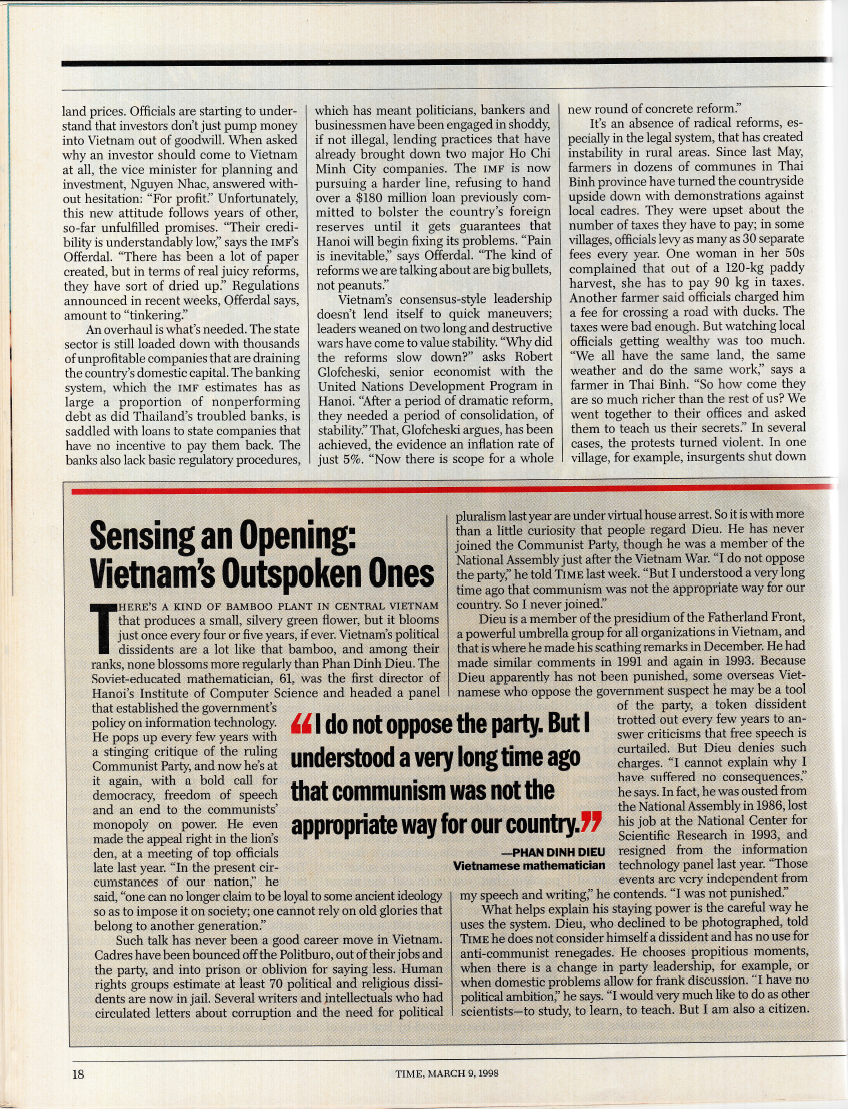
\includegraphics[scale=0.3]{Photos/Time1}
 \end{figure}
 

{\huge  Sensing an Opening: Vietnam’s Outspoken Ones}

\epigraph{I do not oppose the party. But I understood a very long time ago that communism was not the appropriate way for our country.}{\textit{PHAN DINH DIEU – Vietnamese mathematician}}




There’s a kind of bamboo plant in central, Vietnam that produces a small, silvery green flower, but it blooms just once every four or five years, if ever, Vietnam’s political dissidents are a lot like that bamboo, and among their ranks, none blossoms more regularly than Phan Dinh Dieu. The Soviet-educated mathematician, 61, was the first director of Hanoi’s Institute of Computer Science and headed a panel that established the gorvernment’s policy on information technology. He pops up every few years with a stinging critique of ruling Communist Party, and now he’s at it again, with a bold call for democracy, freedom of speech and an end to the communists’ monopoly on power,. He even made the appeal right in the lion’s den, at a meeting of top officials late last year. “In the present circumstances of our nation,” he said, “one can no longer claim to be loyal to some ancient ideology so as to impose it on society; one cannot rely on old glories that belong to another generation.”

 Such talk has never been a good career move in Vietnam. Cadres have been bounced off the Politburo, out of their jobs and the party, and into prison or oblivion for saying less. Human rights groups estimate at least 70 political and religious dissidents are now in jail. Several writers and intellectuals who had circulated letters about corruption and the need for political pluralism last year are under virtual house arrest. So it is with more than a little curiosity that people regard Dieu. He has never joined the Communist Party, though he was a member of the National Assembly just after the Vietnam War. “I do not oppose the party,” he told TIME last week. “But I understood a very long time ago that communism was not the appropriate way for our country. So I never joined.”
 
 Dieu is a member of presidium of Fatherland Front, a powerful umbrella group for all organizations in Vietnam, and that is where he made his scathing remarks in December. He had made similar comments in 1991 and again in 1993. Because Dieu apparently has not been punished, some overseas Vietnamese who oppose the government suspect he may be a tool of the party, a token dissident trotted out every few years to answer criticisms that free speech is curtailed. But Dieu denies such charges. “I cannot explain why I have suffered no consequences,” he says. In fact, he was ousted from the National Assembly in 1986, lost his job at the National Center for Scientific Research in 1993, and resigned from the information technology panel last year. “Those events are very independent from my speech and writing,” he contends. “I was not punished.”
 
 What helps explain his staying power is the careful way he uses the system. Dieu, who declined to be photographed, told TIME he does not consider himself a dissident and has no use for anti-communist renegades. He chooses propitious moments, when there is a change in party leadership, for example, or when domestic problems allow for frank discussion. “I have no political ambition,” he says. “I would very much like to do as other scientists – to study, to learn, to teach. But I am also a citizen. I have to contribute to the life of our country.”
 
A confluence of events-rural unrest in Thai Binh province, an economic downturn and the installation last year of a new leadership-seems to have inspired others, like Dieu, to express their dissent. A retired general, Tran Do, wrote an open letter to party leaders, warning, “If we do not kick our-selves out of this sickly morass we will collapse…and if we let the morass linger on, then we will have increasing social instability.” In a letter to the party leadership, Hoang Huu Nhan, a former high-ranking economics adviser to the party, has called for more dramatic economic reforms. “People seem to be emboldened,” says Carlyle Thayer, an Australian scholar of Vietnamese politics. “It’s a time of fluidity, and that’s a time for people to get ideas out.” Dieu insists he has not been in communication with Tran Do or Nhan. Thayer suspects, however, that “there are probably many people who agree with him and who invited him to say what they don’t want to be identified with themselves.”

In recent years, the door has sometimes opened a crack to allow such debate, but then closed just as quickly. In the late 1980s, political discourse was relaxed-until Vietnamese leaders saw communist government toppling in Eastern Europe. Dieu and others spoke out during a 1991 leadership change. This time, the new Party General Secretary, Le Kha Phieu, has met with Tran Do and with dissident Hoang Minh Chinh, who has been in and out of prison since the 1960s, according to sources close to the two men. None of these meetings, or speeches like Dieu’s, are publicized in Vietnam’s state-run media, and some prominent writers and journalists have been warned by police not to have contact with Tran Do or Dieu. But the Foreign Ministry, in a written response to questions from foreign journalists, says such criticisms of the party are merely “a normal thing.” A septuagenarian writer is cheered that so far the government hasn’t been responding as it normally does, by cracking down on dissidents. “For 40 years, I have lived on the fringes of society,” he say. But still I have hope. Our current crisis means not all of the leaders can be deaf. Before, they would have thrown this stuff in a trash bin and disciplined the authors. Now, the leave them alone.”

 Many younger Vietnamese are less sanguine. “The party views these people like mosquitoes,” says a writer in his 30s whose bleak portrayals of a disintegrating society have irritated authorities. “They annoy you, but they can’t kill you.” What remains to be seen is whether the vocal dissenters will suffer the same fate as the rarely blooming bamboo plant: after it flowers, it usually dies. Dieu, however, is a survivor. “If I can say what I believe,” he says, “then other people can voice their opinions too, and maybe we can have the beginning of democracy.”
-By Tim Larimer/Hanoi

\newpage

%\chapter*{Báo TIME 1998} \index{Báo chí}
 \begin{figure}
 \centering
 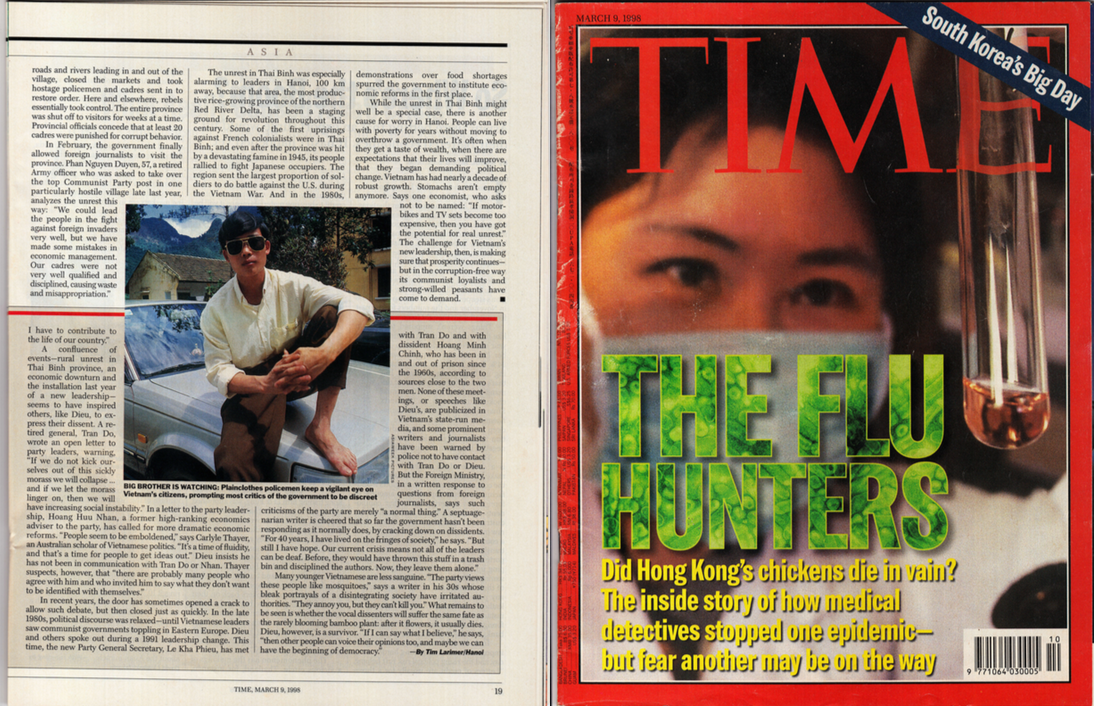
\includegraphics[scale=0.3]{Photos/Time2}
 \end{figure}
 
{\huge Cảm nhận một bước mở cửa: Những người nói thẳng ở Việt Nam}

\epigraph{Tôi không chống Đảng. Nhưng đã từ rất lâu tôi hiểu rằng chủ nghĩa cộng sản không phải là con đường thích hợp với đất nước tôi.}{\textit{PHAN ĐÌNH DIỆU - Nhà Toán học Việt nam }}




    Có một loại cây tre mọc ở miền Trung Việt nam nở một thứ hoa màu xanh ánh bạc rất bé, nhưng có nở thì cũng khoảng bốn năm năm mới nở một lần. Những nhân vật ly khai chính trị của Việt nam khá giống như loài tre đó và trong số họ, không ai trổ hoa đều đặn hơn ông Phan Đình Diệu. Nhà toán học từng học ở Liên Xô, 61 tuổi, ông ta là Viện trưởng đầu tiên của Viện Tin học Hà Nội và đứng đầu một nhóm soạn thảo chính sách của Chính phủ về Công nghệ thông tin. Cứ mỗi vài năm ông ta lại bất ngờ xuất hiện với một sự phê phán sắc bén đối với Đảng Cộng sản cầm quyền, và lần này lại xuất hiện với một lời kêu gọi đậm nét hơn cho dân chủ, tự do ngôn luận, và chấm dứt sự độc tài cộng sản ở chính quyền. Ông ta đưa ra lời kêu gọi đó ngay trong hang sư tử, tại một cuộc họp của nhiều quan chức cao cấp vào cuối năm ngoái . ‘‘Trong điều kiện nước ta hiện nay”, ông ta nói “không thể tiếp tục vin vào lý do trung thành để áp đặt một ý thức hệ lỗi thời cho xã hội, không thể dựa mãi vào những vinh quang dĩ vãng của một thế hệ đi trước”.
    
    Kiểu nói như vậy chưa bao giờ đưa tới một sự nghiệp thăng tiến ở Việt Nam. Có những cán bộ đã bị đưa ra khỏi Bộ Chính trị, bị tước chức vụ và bị khai trừ khỏi Đảng, bị đưa vào tù hoặc vào sự quên lãng để ít nói hơn. Các nhóm nhân quyền đánh giá có ít nhất 70 nhân vật ly khai chính trị và tôn giáo hiện đang bị cầm tù. Một số nhà văn và tri thức phân phát kiểu chuyển tay các bức thư về tham nhũng và yêu cầu đa nguyên chính trị năm ngoái bị quản thúc tại nhà. Chính vì thế mà với ít nhiều tò mò người ta nhìn vào ông Diệu. Ông ta chưa bao giờ vào Đảng Cộng sản, mặc dầu đã là đại biểu Quốc hội ngay sau cuộc chiến tranh Việt nam. “Tôi không chống Đảng”, ông ta nói với TIME tuần trước, “nhưng đã từ rất lâu tôi hiểu rằng chủ nghĩa cộng sản không phải là con đường thích hợp với đất nước tôi. Vì vậy mà không bao giờ tôi vào Đảng”.
    
    Diệu là một ủy viên đoàn chủ tịch Mặt trận Tổ quốc, một hình thức bao trùm lên tất cả các tổ chức ở Việt nam, và đây là nơi mà ông ta đưa ra những lời phê phán gay gắt hồi tháng Chạp vừa qua. Ông ta đã làm những phê bình tương tự vào năm 1991 và lại tiếp tục năm 1993. Vì ông Diệu chưa bị trừng phạt một cách công khai, nên một số người Việt hải ngoại chống chính phủ ngờ rằng ông ta có thể là một công cụ của Đảng, một kẻ ly khai giả mạo, cứ vài năm lại tung ra một lần để trả lời lại những phê phán cho là ngôn luận tự do bi bóp nghẹt. Nhưng ông Diệu bác bỏ những lời buộc tội đó. “Tôi không thể giải thích tại sao tôi chưa phải chịu các hậu quả”, ông ta nói. Thực tế, ông ta đã bị loại ra khỏi quốc hội năm 1981, bị mất chức ở Viện Khoa học Việt  nam 1993, và đã từ chức khỏi Ban Chỉ đạo Quốc gia về công nghệ thông tin năm ngoái. Nhưng ông ta khẳng định: “Những việc đó là hoàn toàn độc lập với những lời nói và bài viết của tôi. Tôi chưa bị trừng phạt”.
    
    Điều giúp ta giải thích cái khả năng bền bỉ của ông ta là ở cái cách thận trọng mà ông ta sử dụng hệ thống. Ông Diệu đã khước từ cho chụp ảnh và nói với TIME rằng ông ta không xem mình là một nhân vật ly khai và không để bị lợi dụng bởi những những người phản kháng chống cộng. Ông ta chọn những thời điểm thuận lợi, khi có một sự thay đổi trong lãnh đạo Đảng chẳng hạn, hay khi những vấn đề trong nước cho phép được thảo luận thẳng thắn. “Tôi không có tham vọng chính trị”, ông ta nói. “Tôi rất muốn được làm như những nhà khoa học khác – nghiên cứu, học tập, giảng dạy. Nhưng tôi cũng là một công dân. Tôi có trách nhiệm đóng góp vào đời sống của đất nước tôi”.

Hàng loạt các sự kiện bất ổn ở vùng nông thôn thuộc tỉnh Thái Bình, kinh tế suy thoái và việc một nhà lãnh đạo nhậm chức đã khiến nhiều người quan tâm như giáo sư Diệu – người đã bày tỏ ý kiến bất đồng. Một tướng quân đội đã nghỉ hưu - ông Trần Độ đã viết thư ngỏ gửi các nhà lãnh đạo Đảng cộng sản, ông cảnh báo: "Nếu chúng ta không tự mình thoát khỏi lý luận giáo điều này chúng ta sẽ sụp đổ và nếu chúng ta cứ để cho lý luận ngày càng bùng nhùng hơn chúng ta sẽ phải chứng kiến những bất ổn xã hội”. Trong một bức thư gửi Lãnh đạo Đảng, ông Hoàng Hữu Nhân – nguyên cố vấn kinh tế cao cấp của Đảng - đã kêu gọi cải cách kinh tế mạnh mẽ hơn nữa. Học giả người Úc nghiên cứu chính trường Việt Nam – ông Carlyle Thayer nói: "Dường như mọi người đã mạnh dạn hơn”. "Đã đến lúc thông thoáng hơn và là lúc để người ta đưa ra quan điểm của mình”. Giáo sư Diệu khẳng định ông không có bất kỳ liên hệ nào với ông Trần Độ và ông Hoàng Nhân. Tuy nhiên, ông Thayer nghi ngờ khi cho rằng: “có thể có nhiều người đồng ý với ông Diệu đã mời ông Diệu phát biểu về những vấn đề mà họ không muốn bị coi là chính họ nêu lên”. 

Trong những năm gần đây, đôi khi cũng có những lúc cởi mở để trao đổi những vấn đề gây tranh cãi nhưng sau đó mọi chuyện khép lại chóng vánh. Cuối những năm 1980, thảo luận chính trị được cởi mở hơn khi các vị lãnh đạo Việt Nam đã chứng kiến chính quyền cộng sản bị lật đổ ở Đông Âu. Giáo sư Diệu và một số người khác đã lên tiếng trong suốt giai đoạn diễn ra thay đổi lãnh đạo năm 1991. Theo một nguồn tin thân cận của hai vị, lần này, tân Tổng Bí thư Lê Khả Phiêu đã gặp tướng Trần Độ và nhà bất đồng chính kiến Hoàng Minh Chính – người mà bị vào tù rồi ra tù suốt những năm 60 -  thông tin về những cuộc gặp hay những phát ngôn của giáo sư Diệu đều không được đăng tải trên các báo chính thống. Một số tay bút kỳ cựu và nhà báo đều được công an Việt Nam cảnh báo không được liên hệ với ông Trần Độ hoặc giáo sư Diệu. Riêng Bộ Ngoại Giao Việt Nam, trong một văn bản trả lời các câu hỏi của các phóng viên nước ngoài nêu những phản biện như vậy đối với Đảng cộng sản đều là những điều “rất bình thường”. Một nhà văn già nói rằng chính phủ Việt Nam không phản ứng như cách thông thường họ làm mà bằng việc đàn áp các nhà bất đồng chính kiến. Ông nói: "Tôi đã sống bên lề xã hội Việt Nam suốt 40 năm nhưng tôi luôn hy vọng. Cơn khủng hoảng hiện nay không có nghĩa mọi nhà Lãnh đạo đều mũ ni che tai. Trước đó, họ đã ném thứ này vào thùng rác và kỷ luật các tác giả. Nhưng bây giờ họ cô lập họ”.

Nhiều thanh niên người Việt không mấy lạc quan cho lắm. Một nhà văn chừng 30 tuổi – người đã có những miêu tả về sự ảm đạm của một xã hội đã khiến các nhà chức trách khó chịu - nói: "Đảng cộng sản luôn coi những người này là những con muỗi. Họ có thể làm phiền anh nhưng không thể giết được anh”. Điều gì còn lại để nhận ra là liệu các nhà bất đồng chính kiến có phải chịu số phận giống cây tre khi sinh sản: sau khi hoa tre nở cây thường chết. Tuy nhiên, giáo sư Diệu là một người sống sót. Ông nói: “Nếu tôi nói điều tôi tin thì người khác cũng có quyền cất lên tiếng nói của mình và đó có thể là sự khởi đầu của một nền dân chủ”.

-By Tim Larimer/Hanoi



\chapter{Mon Dieu!  (Far Easrten Economic Review 08/1993)}
\begin{figure}
\centering

\includegraphics[scale=.4]{Photos/FE1}
\end{figure}  
  
  
\textbf{INTELLIGENCE}\\
\textbf{Adieu Dr Dieu}


Vietnamese mathematician, long the most outspoken critic of the ruling Communist Party to remain out of prison, has been ousted from his post as vice-chairman of the National Centre for Scientific Research. In recent months, Dieu had called for the party to abandon its Marxist-Leninist ideology and challenged it to allow other parties to compete in the country’s political life. Officially, he was removed from his post in a dispute with the centre’s director physicist Nguyen Van Hieu, but observers see Dieu’s firing as an attempt by the party to isolate him from potential supporters, Dieu has asked to be allowed to teach mathematics and computer science at Hanoi University. 




\textbf{VIETNAM}\\

 Mon Dieu!


\textbf{FROM OUT SOUTH-EAST ASIA CORRESPONDENT    \quad           HANOI}


Sitting in his book-lined study in Hanoi, Phan Dinh Dieu looks the very model of academic detachment. Mr Dieu is a professor of mathematics and a respected figure in Hanoi. But he is also probably the most outspoken advocate of political reform in Vietnam to remain out of prison. 


In recent years the number of political prisoners has decreased. All the same, Asia Watch, an American human-rights group, estimates that Vietnam has “hundreds if not thousands of political and religious prisoners”. This year eight dissidents were jailed for circulating a newsletter called \textit{Freedom Forum}, which called  for multi-party democracy. Doan Viet Hoat, the group’s leading figure, got 15 years. 


As a man who spent the Vietnam war in the north and who has worked within the system (without ever joining the Communist Party), Mr Dieu is granted some latitude. But he recently lost his job as vice-president of the National Centre for Scientific Research in Hanoi. The official reason is that he had a dispute with the centre’s director, but some think that the party may be trying to isolate Mr Dieu from students. Still, somebody in the government is clearly not averse to giving Mr Dieu a platform. His meeting with \textit{The Economist} was arranged by the foreign ministry’s press service and watched over by an official guide. 


Alongside the learned papers and football magazines on Mr Dieu’s shelves are the works of Vaclav Havel and Andrei Sakharov. This is an act of boldness in itself. The evidence used against convicted dissidents has included articles in their possession about the upheavals in Eastern Europe. For Vietnam’s leader the lesson of Eastern Europe was clear: press ahead with economic reform but keep politics frozen. Mr Dieu is inclined to disagree, although he is careful to offer his views as part of a scientific rather that a political debate. He says, 
\begin{quote}
\textit{The threat of chaos is real in Vietnam, and the concern of people in the party is to achieve stability. I agree that we need stability, but of what kind? Scientifically, we can differ on that, they have a static view a stability. A more scientific concept is dynamic stability achieved through evolution. It is impossible in principle to have economic development and not have political development. The market economy contradicts communism. If you accept market economics sooner or later you have to abandon the principles of communist society: one unique party in power, the dominant role of the public sector and so on. }
\end{quote}

Some theorists in Asia suggest that communism in Vietnam and China will not collapse as it has in Eastern Europe. They believe economic reform can be combined with single-party rule for years to come. The ruling parties will simply ditch the ideological baggage of communism and adopt the authoritartianism of Singapore or Taiwan. 


Mr Dieu is not convinced. Like most patriotic Vietnamese, he instinctively shies away from any comparison to China. Nor are Singapore and Taiwan good models, according to Mr Dieu. “The ruling parties there evolved in very different circumstances from today. The spirit of democracy is now much stronger in our area than it was 20 years ago.” Events in Taiwan this week (see page 25) tend to support his view. 


Mr Dieu is hopeful about the growth of pluralism in Vietnam. He says that discussions within the party are much freer than they were a couple of years ago; it is now possible to study the principles of social democracy or the crisis of Marxism. At official seminars concepts like multi-party democracy have been aired. “We can discuss these things in private. Whether the party accepts them or not is another matter,” he says, amid gales of nervous laughter. 

\begin{figure}
\centering
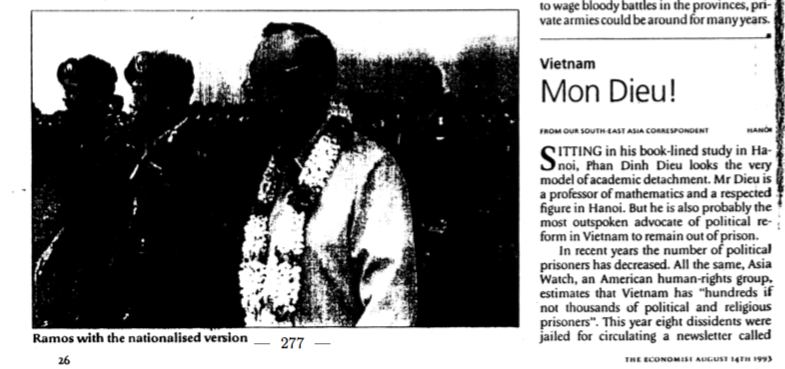
\includegraphics[scale=.4]{Photos/FE2}
\end{figure}  
  

\newpage
TIN TÌNH BÁO


Tạm biệt Giáo sư Diệu (Adieu Dr Dieu)


Nhà toán học Việt Nam, nhà phê bình kiên trì và thẳng thắn nhất về Đảng Cộng sản đang cầm quyền chưa khi nào bị tù đày nhưng đã bị giáng chức Phó Viện Trưởng Viện Hàn Lâm Khoa Học Việt Nam. Những tháng gần đây, giáo sư Diệu đã kêu gọi Đảng cộng sản hãy từ bỏ ý thức hệ Marxist-Leninist và để cho các đảng khác có cơ hội canh tranh trong đời sống chính trị của đất nước. Lý do chính thức khiến ông đã bị giáng chức sau khi tranh luận với vị Giám đốc Trung tâm cũng là nhà vật lý tên là Nguyễn Văn Hiệu. Tuy nhiên các nhà quan sát nhận định việc cho ông Diệu thôi chức tước là để cô lập ông với các nhà ủng hộ tiềm năng. Giáo sư Diệu cũng yêu cầu được tiếp tục công việc giảng dạy toán học và khoa học máy tính tại trường Đại học ở Hà nội. 


\noindent \textbf{VIỆT NAM}\\
Ông Diệu


\begin{center}
PHÓNG VIÊN TỪ TRUNG TÂM ĐÔNG NAM Á - HÀ NỘI 
\end{center}

Ngồi cùng ông trong căn phòng đầy sách tại Hà Nội, Giáo sư Phan Đình Diệu toát lên dáng vẻ của một nhà học thuật độc lập. Ông là một Giáo sư toán học và là một gương mặt đáng kính ở thủ đô Hà Nội. Nhưng ông cũng là người ủng hộ thẳng thắn nhất cho cải cách chính trị ở Việt Nam mà vẫn được tự do. 


Trong những năm gần đây số lượng tù nhân chính trị đã giảm. Cùng nhận xét trên, Asia Watch - tổ chức nhân quyền của Mỹ ước tính Việt Nam có "hàng trăm nếu không muốn nói là hàng ngàn tù nhân chính trị và tôn giáo". Năm nay, tám nhà bất đồng chính kiến bị bắt giam vì đã phát hành trang tin có tên Diễn đàn Tự Do kêu gọi dân chủ đa nguyên đa đảng dưới sự khởi xướng của ong Đoàn Viết Hoạt - người đã phải nhận mức án 15 năm tù. 


Là người đã từng tham gia chiến đấu ở miền Bắc Việt Nam và làm việc trong hệ thống (chưa bao giờ gia nhập Đảng Cộng sản), Giáo sư Diệu cũng được trao một số quyền nhất định, tuy nhiên gần đây ông đã bị mất chức Phó Viện Trưởng Viện Hàn Lâm Khoa Học Việt Nam. Lý do chính thức đưa ra là ông đã có một cuộc tranh cãi với vị Giám đốc Trung tâm này tuy nhiên nhiều người cho rằng có lẽ Đảng muốn tách giáo sư Diệu khỏi sinh viên. Rõ ràng nhiều vị trong chính phủ tỏ rõ thái độ không muốn dành cho ông Diệu bất kỳ diễn đàn nào. Cuộc gặp của ông với tờ báo Kinh tế gia là do cơ quan báo chí thuộc Bộ ngoại giao sắp đặt và luôn bị giám sát. 


Cùng với các bài báo đã đọc và một số tạp chí bóng đá trên giá sách tại nhà giáo sư còn có các tác phẩm của Vaclav Havel và Andrei Sakharov. Đây có thể nói là một hành động táo bạo. Bằng chứng để chống lại các nhà bất đồng chính kiến đã ​​bị kết án gồm các bài viết của chính họ về cuộc binh biến ở Đông Âu. Và các nhà lãnh đạo của Việt Nam đã có một bài học rõ ràng từ Đông Âu là thúc ép đổi mới kinh tế nhưng chính trị thì bất động. Ông tỏ rõ thái độ bất đồng quan điểm trên mặc dù ông rất thận trọng khi đưa ra quan điểm của mình với góc nhìn của một nhà khoa học hơn là một cuộc tranh luận chính trị.


Mối đe dọa về sự bất ổn ở Việt Nam là có thật và mối quan ngại của nhiều người trong Đảng cộng sản là làm sao phải giữ được sự ổn định. Tôi hoàn toàn nhất trí việc chúng ta phải có sự ổn định nhưng ổn định như thế nào?. Về mặt khoa học, chúng ta cần phân biệt rõ là họ có một cái nhìn cố định về sự ổn định. Một khái niệm khoa học là cần phải đạt được sự ổn định trong thể động thông qua tiến trình vận động. Về mặt nguyên lý, không thể có một sự phát triển kinh tế tách rời sự vận động của chính trị. Kinh tế thị trường mâu thuẫn với chủ nghĩa cộng sản. Nếu anh chấp nhận nền kinh tế thị trường thì sớm hay muộn anh cũng phải dừng ngay các nguyên lý của xã hội cộng sản đó là tồn tại duy nhất một Đảng, vai trò phủ bóng của khu vực công và nhiều điều khác. 


Một số nhà lý thuyết ở châu Á cho rằng chủ nghĩa cộng sản ở Việt Nam và Trung Quốc sẽ không sụp đổ như ở Đông Âu. Họ cho rằng cải cách kinh tế có thể được kết hợp với sự nắm quyền hành của một đảng trong nhiều năm tới. Một cách đơn giản là các đảng cầm quyền chỉ cần dẹp đi mớ lý luận về chủ nghĩa cộng sản và thích nghi ngay với chủ nghĩa độc đoán như của Singapore hoặc Đài Loan.


Việc lý giải như vậy không thuyết phục được Giáo sư. Giống như hầu hết người Việt Nam yêu nước, ông tránh xa mọi so sánh với Trung Quốc, Singapore hay Đài Loan vì theo Ông: “Các đảng cầm quyền đang vận động theo bối cảnh khác nhau không giống với ngày nay. Hiện nay tinh thần dân chủ đang dần lớn mạnh trong khu vực so với 20 năm trước”. Các sự kiện trong tuần qua tại Đài Loan (xem trang 25) minh họa cho quan điểm của Giáo sư.


Giáo sư luôn hy vọng về sự phát triển đa nguyên, đa đảng ở Việt Nam. Ông nhận định các cuộc thảo luận trong nội bộ Đảng giờ đây đã cởi mở hơn so với cách đây nhiều năm. Giờ là lúc có thể nghiên cứu về các nguyên lý của dân chủ xã hội hoặc cuộc khủng hoảng của chủ nghĩa Mác. Tại các cuộc họp quan chức cũng đã xuất hiện những tiếng nói về nền dân chủ đa đảng. Giáo sư vừa nói vừa cười sảng khoái: “Chúng ta có thể thảo luận những vấn đề trên theo một cách riêng. Còn việc Đảng có chấp nhận hay không là một việc khác”./. 



\chapter{Bài thơ theo suốt cuộc đời tôi (Phan Thị Hà Dương)}
Nguồn: \href{https://vietnamnet.vn/vn/giao-duc/nguoi-thay/gs-phan-dinh-dieu-qua-hoi-uc-cua-con-gai-710146.html}{Bài thơ theo suốt cuộc đời nhà toán học Phan Thị Hà Dương - VietnamNet} và \href{https://vietnamnet.vn/vn/giao-duc/nguoi-thay/gs-phan-dinh-dieu-day-con-710149.html}{Bài học sâu sắc mà GS Phan Đình Diệu dạy con gái - VietnamNet}

\paragraph{Bài thơ theo suốt cuộc đời nhà toán học Phan Thị Hà Dương - VietnamNet} \ \\

"... Nhưng tôi nhớ, chẳng bao giờ tôi có thể quên, bài thơ đầu tiên mà tôi tự cầm sách đọc, đọc và yêu thích, đọc và ghi nhớ, đọc và mang theo suốt cuộc đời. Đó là "Buổi sơ khai"...."

LTS: "Màu sắc của bìa sách, cả việc cuốn sách được bọc và nét chữ của bố như chìm vào bìa mang đến cho tôi một cảm giác trân trọng trang nghiêm và mênh mang" - Ấn tượng sâu đậm nhất về người bố - GS. Phan Đình Diệu - nhà toán học và là người đặt nền móng cho ngành Tin học của Việt Nam, trong hồi ức của người con - cũng là một người làm toán - hoá ra lại không phải về toán mà là... văn. Văn chương, và đặc biệt thơ ca, nơi những cảm xúc trái ngược quyện lại hài hòa, nơi điều gần gụi và cái vô cùng ở sát bên nhau, đã hình thành nên con người và gắn kết sâu sắc thêm tình cha con. 

Báo VietNamNet xin trân trọng giới thiệu hồi ức của nhà toán học Phan Thị Hà Dương về người bố đáng kính của mình.

\paragraph{Bài thơ theo suốt cuộc đời nhà toán học Phan Thị Hà Dương} \ \\

Tôi không còn nhớ bài thơ đầu tiên tôi được học là bài nào, có lẽ đó sẽ là một bài từ thời mẫu giáo, hay xa hơn nữa từ thời nhà trẻ, vì tôi, như tất cả bọn trẻ con thời ấy, đều đi nhà trẻ từ ngày một tuổi.

Tôi không còn nhớ lần đầu tiên tôi biết đọc là khi nào, có thể là trước khi đến trường, vì tôi, như tất cả bọn trẻ con muôn đời, thích tập đọc những bảng chỉ đường, những biển hiệu dọc phố.

Nhưng tôi nhớ, chẳng bao giờ tôi có thể quên, bài thơ đầu tiên mà tôi tự cầm sách đọc, đọc và yêu thích, đọc và ghi nhớ, đọc và mang theo suốt cuộc đời. Đó là "Buổi sơ khai".

Ngày ấy, tôi, con bé con 8 tuổi, mùa hè mặc váy trắng, nằm trên sàn nhà lát những viên gạch đỏ trong phòng ngoài một căn hộ nhỏ trên tầng 4 khu Giảng Võ. Bố tôi cầm một cuốn sách, hình như bìa màu trắng bạc, không có hình vẽ gì, chỉ một dòng chữ nhỏ: “Thơ Tagore”. Bố tôi đưa tôi và chỉ vào một bài thơ: ”Bài này hay lắm, con đọc đi".

Tôi đã đọc bài thơ trong những hình ảnh thiêng liêng về một nhà thơ râu tóc bạc phơ, hiền từ và đẹp như một vị thánh; về sự ngưỡng mộ sùng kính của những người đọc thơ, khi đến thăm ông lúc về đã đi giật lùi. Những câu chuyện bố kể như in vào đầu tôi, con bé con 8 tuổi, về sự linh thiêng và cao quý của Nhà Thơ.

Tôi đã đọc bài thơ, và ngay những dòng đầu đã thích chí cười với “mẹ ôm chặt bé vào lòng và trả lời nửa cười nửa khóc”. Tôi còn nhớ như in cảm giác sung sướng của đứa bé là tôi lúc ấy khi thấy hình ảnh vừa cười vừa khóc, khi cảm thấy mình hiểu được sự mâu thuẫn của hình ảnh vừa mừng vui, vừa ngộ nghĩnh, vừa xúc động.

Tôi còn nhớ tôi đã hỏi mẹ “ban thờ” là gì và khi mẹ trả lời tôi thấy thật hay biết bao khi trong thơ có những từ thật là lạ, và “ban thờ” là một điều gì đó cao xa hơn nhiều những từ mà tôi biết, “ban thờ” chứ không phải “bàn thờ”.

Tôi còn nhớ “và trong cả cuộc đời của mẹ mẹ nữa kia” đã gieo vào tôi ý niệm về một cái gì đó lồng vào nhau, mẹ của mẹ, mẹ của mẹ của mẹ, và xa nữa, xa xa nữa…

Tôi còn nhớ, mỗi lần tôi đọc bài thơ này cho bố mẹ, cho cả nhà nghe, đến đoạn “khi đương thời con gái”, thể nào mẹ tôi cũng đọc cùng tôi, và gương mặt mẹ bừng lên rạng rỡ.

Tôi đã đọc, tôi đã đọc nhiều lắm, tôi không biết vì sao mình lại thích bài thơ này đến vậy. Lúc nào tôi cũng đọc. Họp mặt khu tập thể, tôi đứng lên ghế đọc cho các cô các bác, các bà nghe. Ngày thi văn nghệ theo các khu nhà các phường, các huyện, tôi diện áo trắng juyp xanh xếp nếp đứng trên bục sân khấu đọc cho cả hội trường nghe. Khi ấy, bọn con trai lớp tôi, những cậu chàng lớp 8, khúc khích cười trêu lúc tôi đặt hai tay lên ngực và đọc “mẹ đã siết chặt con trên ngực mẹ”.


Tôi đã đọc những đêm ru con ngủ những ngày đầu làm mẹ. Dẫu rằng bài thơ trúc trắc nhường này nhưng với tôi nó vẫn êm dịu xiết bao. Khi ấy, mẹ tôi, giờ đây đã là mẹ của mẹ, có lẽ lại như ngày xưa nhẩm cùng tôi đoaanj "khi đương thời con gái".

Có thể là ngày bé tôi đã chỉ hiểu lơ mơ. Có thể là với thời gian, tôi đã thấm hiểu niềm hạnh phúc trong câu trả lời nửa cười nửa khóc. Có thể là đến bây giờ, khi tôi đã có hai con, tôi vẫn chưa hiểu hết bài thơ.

Nhưng tôi luôn thầm cám ơn bố mẹ đã cho tôi đọc bài thơ này vào buổi sơ khai của cuộc sống tâm hồn. Để tôi, trong dấu ấn đầu tiên của tâm hồn mình, trong những bước tiếp theo và mãi mãi, luôn mơ màng rằng trong thơ có ẩn chứa những từ ngữ cao xa, những từ ngữ đa nghĩa, rằng trong thơ những cảm xúc trái ngược, những cảm xúc mâu thuẫn bỗng quyện lại hài hòa, rằng trong thơ điều gần gụi và cái vô cùng sát bên nhau đến thế. Và nếu như nhà thơ viết một bài thơ không chỉ bằng một phút giây tỏa sáng mà bằng một phút giây tỏa sáng cộng với cả cuộc đời mình; thì người đọc thơ đọc một bài thơ không chỉ bằng một đêm xuân khi hình như mưa lất phất bay mà bằng một đêm xuân mưa lất phất bay cộng với cả cuộc đời mình.

Buổi sơ khai

Bé hỏi mẹ:

“Mẹ ơi, con từ đâu đến vậy

Mẹ đã nhặt được con ở tận nơi nào ?”

Mẹ ôm chặt bé vào lòng, và trả lời

nửa cười nửa khóc:

“Con ơi con, con đã được giấu kín trong lòng mẹ

như chính những thèm khát ước mơ của nó.

Con ở trong con búp bê của những món đồ chơi tuổi nhỏ của mẹ.

Và mỗi buổi sáng khi mẹ lấy đất sét nặn ra

hình ảnh Chúa Đời của mẹ

thì mẹ đã nặn đi nặn lại con rồi

Con ở trên ban thờ nơi thờ vị thổ thần

Và khi thờ thần đó, đồng thời mẹ cũng thờ con

Con đã sống trong tất cả mọi niềm hy vọng, thương yêu trong đời mẹ

và trong cuộc đời của mẹ mẹ nữa kia

Con đã được nuôi dưỡng đời này qua đời khác

trong lòng của vị thần linh bất tử đã ngự trị ở nhà ta.

Khi đương thời con gái, trái tim mẹ nở xòe như một đóa hoa.

Con đã lượn quanh nó như một mùi hương phảng phất

Vẻ tươi mát nhẹ nhàng của con

Nở trên chân tay non trẻ của mẹ

như một ánh hồng

trên trời cao

trước buổi bình minh

Con là đứa con cưng của Thượng đế,

là anh em sinh đôi với ánh bình minh

Con đã theo dòng nước trôi xuống cuộc đời trần tục này

và cuối cùng con đã được đặt vào trong lòng mẹ

Khi mẹ ngây nhìn khuôn mặt của con

mẹ như bị ngập trong bao điều bí ẩn,

Và con, vốn là của chung của tất cả mọi người

đã trở thành của riêng của mẹ

Sợ mất con đi, mẹ đã siết chặt con trên ngực mẹ

Không hiểu sự diệu kỳ nào

Đã chiếm lĩnh cái kho vàng trên cõi thế

và đặt con vào đôi tay mảnh khảnh của mẹ đây ?”

(Thơ Tagore, Đào Xuân Quý dịch) 

\paragraph{Bài học sâu sắc mà GS Phan Đình Diệu dạy con gái - VietnamNet}

Trong ký ức của nhà toán học Phan Thị Hà Dương, chỉ có một lần duy nhất GS Phan Đình Diệu - can thiệp vào việc học văn của con gái: “Bố muốn con hiểu rằng con chỉ nên viết ra những gì mà con thực sự nghĩ là đúng”.

Thời phổ thông, có nhiều lúc tôi ngán mớ đời khi có đứa bạn hay thậm chí thầy giáo hỏi có phải cái bài toán về nhà tôi nhờ bố nên mới giải được, trong khi thực ra toàn bộ đời đi học của tôi chỉ có hai bài nhờ bố giải. Ngay cả khi tôi hỏi bố nên học toán hay tin học thì bố cũng bảo: “Bố tôn trọng mọi quyết định của con”.

Vậy mà trong thâm tâm tôi luôn nghĩ bố là người thầy dạy mình học văn dù rằng chỉ có một lần duy nhất bố can thiệp vào việc học văn của tôi.

Lần ấy tôi bị 4 điểm bài văn kiểm tra chất lượng đầu năm lớp 6. Trước đấy, mặc dù cứ thích đọc thơ và suốt ngày ôm truyện nhưng đi học thì tôi chỉ khoái môn toán nên cũng chẳng ghét bỏ hay yêu quý gì môn văn, có khi tôi được 9 điểm cao nhất hồi lớp 3 khi vô cùng xúc động làm bài văn về anh Lê Văn Tám, cũng có khi tôi làm lục bát ngang phè vào hồi lớp 5. Nói chung không có vấn đề gì nghiêm trọng.

Nhưng 4 điểm, lần đầu tiên dưới trung bình, là chuyện tày đình, và vì thế lần đầu tiên bố đọc bài văn của tôi. Tôi vẫn nhớ có một câu đề bài là “Hãy viết một câu văn hay, sử dụng biện pháp nhân cách hóa” và tôi đã chép nguyên xi một trong các câu mẫu của cô “những dãy nhà tường trắng mái đỏ của trường em trông như những chú lùn đội mũ đỏ”. 

Bố bảo tôi: “Bố không thấy câu văn này hay ở chỗ nào”. Tôi lý sự: “Nhưng chính cô cho bọn con học câu mẫu, bây giờ con chép lại thì cô lại trừ điểm”. Bố nhìn tôi rất nghiêm trang và hỏi: “Thế con có thấy những dãy nhà ở trường giống các chú lùn không?”. Tôi lí nhí: “Nhưng mà cô ...”. "Không, bố hỏi con cơ, con có thấy thế không?”. Tôi được dịp bùng ra: “Không ạ, con chẳng thấy giống gì cả, nhà thì dài dằng dặc, như cái hộp, chẳng biết sao cô lại cho như thế, chỉ tại cái nhân cách hóa thôi ạ!".

Lúc ấy bố nhìn tôi rất thẳng và bảo tôi: “Bố muốn con hiểu rằng con chỉ nên viết ra những gì mà con thực sự nghĩ là đúng.”

Còn tôi làm nũng bố: “Con chẳng biết thế nào là một câu văn hay cả”.  

Bố nói rằng sao bố thấy con suốt ngày đọc truyện mà bây giờ đến một câu văn hay cũng không biết, con đang đọc truyện gì vậy. Thật là xui xẻo cho tôi, cái thời đấy thì vớ được gì đọc nấy chứ có nhiều lựa chọn đâu (hồi ấy phải có người quen mới mua được truyện từ NXB mà). Nếu mà cách đấy mươi ngày, tôi đang đọc “Tôm Giôn- đứa trẻ vô thừa nhận” tập 1 (tập 2 và 3 phải cả năm sau mới được đọc) thì đã chẳng vấn đề gì, đằng này lúc ấy tôi lại đang một gối hai quyển dày cộm “Ghenny Ghéchac” và “Hoa hậu xứ Mường”. Bố không bằng lòng một chút nào, bố bảo rằng xưa nay bố để tôi tự do đọc sách nhưng vì bây giờ tôi không biết viết một câu văn nữa nên bố mới phải quan tâm đến việc này, và rằng hai cuốn này không phù hợp với tôi. Dù tôi đã năn nỉ bố là đang đúng đoạn hồi hộp và truyện sắp phải trả rồi nhưng bố kiên quyết không.

Rồi bố bảo: “Nếu con muốn biết thế nào là một câu văn hay thì con có thể đọc cuốn này”, và bố rút trên giá sách xuống một cuốn sách. Đến bây giờ tôi vẫn nhớ cảm giác khi cầm cuốn sách đó. Một cuốn sách khá mỏng, bìa được bọc bằng giấy nâu, kiểu giấy xi măng ngày xưa, ở gáy sách và ở bìa sách, phía chếch lên bên phải là những nét chữ in của bố, nét chữ mực màu đen: “GIÓ ĐẦU MÙA”. Màu sắc của bìa sách, cả việc cuốn sách được bọc và nét chữ của bố như chìm vào bìa mang đến cho tôi môt cảm giác trân trọng trang nghiêm và mênh mang.

Tôi vẫn nhớ hai truyện đầu tiên là “Nhà mẹ Lê” và “Hai đứa trẻ”, chỉ có điều tôi không nhớ là truyện nào trước truyện nào sau (có lần tôi tranh luận với một bạn, tôi nói “Nhà mẹ Lê mình nhớ rõ ràng” còn nó bảo “Hai đứa trẻ không thể sai được”, cuối cùng cùng với thời gian thì ý kiến của nó hòa vào với tôi đến nỗi bây giờ tôi mới chẳng còn nhớ gì thế này).

Sau này, theo trí nhớ của tôi, tôi đã luôn tự viết các bài văn mà chẳng bao giờ chép lại từ đâu cả, và có vẻ là tôi còn rất tự tin nữa cơ.

Sau Thạch Lam, tôi quá háo hức, và đã quét sạch cả một ngăn giá sách của bố, đầu tiên là mấy tập tuyển tập Nam Cao, tôi thấy buồn quá và cũng nhiều chuyện không hiểu được, rồi thích nhất là hai (hay ba) tập Nguyễn Công Hoan, văn ông rất sinh động, nhiều đối thoại; rồi Thế Lữ. Thế Lữ cả thơ và văn chỉ một quyển, rất dày. Phần đầu là thơ, mở đầu bằng “Nhớ rừng”, phần sau là văn. Tôi kể cho bố nghe tôi khoái chí thế nào khi đọc “Những nét chữ” và “Vàng và máu”, bố bảo hồi sinh viên bố cũng rất thích đọc truyện trinh thám của Thế Lữ. Bố mẹ và cả nhà rất thích nghe tôi đọc “Nhớ rừng”, tôi bé con mà rất thích đọc hùng tráng, còn bố thích đọc “Tiếng trúc tuyệt vời”, tôi vẫn nhớ những lúc bố đọc:

“Cô em đứng bên hồ

nghiêng tựa mình cây, dáng thẩn thơ

Chừng cô tưởng đến ngày vui sẽ mất,

mà sắc đẹp rỡ ràng rồi sẽ tắt

Cho nên khi cô nghe tiếng trúc tuyệt vời

Thổn thức với lòng cô thổn thức

Man mác với lòng cô man mác

Cô để tâm hồn tê tái bâng khuâng ..."

Và bố hỏi tôi có biết vì sao lại gọi là “cô em” mà không phải là “cô” hay “em” không, nhưng hình như bố không trả lời. Sau này, khi đọc Thi nhân Việt Nam tôi có thấy Hoài Thanh bình chữ này.

Ngày ấy, đi đâu bố cũng xách tôi theo, tôi đi gặp những ông Moi Sép, cô Linđa, tôi lên Đồi Thông, tôi đến Nghĩa Đô.

Hồi tôi mới ở Pháp về Viện Toán làm việc, có lần tôi đang đứng ở bảng thông báo đọc linh tinh thì bỗng nghe: “Em có phải là Hà Dương không, sao em lại ở đây, trông em chẳng khác cái hồi 9 tuổi hay lên Viện đọc thơ gì cả”. Tôi buồn cười quá, vì tôi nghĩ là mình rất khác, thậm chí khác với vài tháng trước đó. Và mặc dù tất nhiên là tôi chẳng nhớ ra anh ấy là ai nhưng tôi vẫn được tặng một bó hoa bất tử đang bày trong phòng làm việc của anh ấy. Bó hoa ấy tôi vẫn để trong phòng làm việc của mình (hơi bụi một tí) như kỷ niệm về một thời 9 tuổi hay lẽo đẽo theo chân bố mẹ.

Một chấm sao không ngủ cuối thiên hà

Ngày trước, những năm 80, những năm cuối cấp một và cấp hai của tôi, nhà tôi ở khu Đồng Xa, bố tôi có rất nhiều bạn bè đến chơi. Chủ nhật nào phòng khách nhà tôi cũng có bạn của bố tôi, những bạn học cũ, bạn toán, bạn văn; những người bạn mới, có những người vì một bài viết của bố tôi mà đã đến rất nhiều chủ nhật và đã trở nên thân thiết.

Tôi vẫn nhớ chiều chủ nhật ấy, trong phòng khách nhà tôi có bố mẹ tôi, có cậu Cương (PGS. Văn Như Cương), có bác Đoàn Quỳnh, bác Hoàng Xuân Sính, có lẽ có cả bác Hà Văn Tấn nữa, và các bác khác. Bố tôi nói: "Mình có tập thơ này hay lắm, của Việt Phương”. Và bố tôi giới thiệu với mọi người một tập bản thảo chép tay của bác Việt Phương, nét bút mực trên nền giấy hơi ngà sẫm màu, các chữ đầu dòng đều không viết hoa, và tên bài thơ nào cũng chỉ là một chữ. Tập thơ ấy không phổ biến và bác đã cho bố mượn.

Bố tôi đọc cho các bạn mình nghe một số bài. Tôi vẫn nhớ không khí của buổi chiều ấy, niềm hứng khởi và sự tâm đắc của bố và các bạn. Theo trí nhớ của tôi thì nhiều bài thơ mang tính trí tuệ và mọi người đã thán phục vì những tứ thơ độc đáo và sâu cay, có những tứ thơ làm mọi người bật lên như một sự khám phá. Nhưng bài thơ mà tôi thích nhất là một bài thơ tình cảm, với một cái tên thật lạ: màu. Tôi vẫn nhớ giọng đọc thơ của bố khi đó, tách khỏi giọng đọc có phần nhấn nhá, đôi khi hơi hài hước và có khi nhấn giọng lúc trước, bài thơ này bố tôi đọc rất tình cảm.

Đến bây giờ tôi vẫn như đang nghe thấy giọng đọc trầm ấm, trìu mến và tình cảm của bố tôi.

em cứ là những tinh mơ tê tái rét

phanh cổ áo ra cho gió siết vào da

em cứ là cơn giông đầu mùa

đi đầu trần đón dòng mưa xối xả

em cứ là cái khoảng cách chập chờn sương phủ

suốt một đời anh vất vả vượt qua

em cứ là giữa mịt mùng vô định

một chấm sao không ngủ cuối thiên hà  

Những tối sau đó, bố tôi còn đọc cho mấy mẹ con nghe, có những bài bố cho tôi đọc nữa. Chỉ hơn một tuần thôi, rồi bố tôi đã trả lại tập bản thảo cho bác Việt Phương. Nhưng bài thơ đã in vào trong trí não tôi.

Sau này, sau những năm 1990, khi nhà tôi đã chuyển, khi những cuộc cách mạng đã nở bừng trên thế giới, khi những biến cố lớn đã đến với biết bao người bạn thân thiết của bố tôi, người ta đã nhắc nhiều hơn đến những bài thơ của bác. Và mãi về sau, khi tập thơ “Cửa đã mở" của bác Việt Phương được in, tôi đã tìm mua, mong nhìn lại những bài thơ hồi bé tôi đã được nghe bố đọc. Tôi tìm thấy những bài như bài “Thịt":

Chị mười ba ý tứ nết na

Cuối bữa cơm gắp rụt rè một miếng

(Ngày trước, khi bố tôi đọc bài này, mẹ tôi hay bảo giống chị tôi, lúc nào cũng nhường nhịn cả nhà).

Có nhiều bài nữa, nhưng tôi không tìm thấy bài thơ trong tâm trí tôi. Và vì thế, có những khi tôi cứ thưởng cho mình cái ý nghĩ rằng chỉ có bố tôi và tôi nhớ bài thơ ấy thôi.

Đến bây giờ tôi vẫn chưa hiểu rõ hết nghĩa của tên bài thơ, nhưng rất nhiều những sáng tinh mơ khi tiết thu đã hết và những làn gió sớm mùa đông siết buốt da, tôi lại phóng trên đường phố Hà Nội, lại bỏ khăn quàng cổ để cảm nhận câu thơ.

Đến bây giờ, khi viết những dòng này, tôi chợt nhận ra vì sao việc đọc một bài thơ đối với tôi có ý nghĩa thiêng liêng đến thế. Tôi đã chịu ảnh hưởng của bố, đã luôn nâng niu từng bài thơ, nâng niu từng giây phút mình đọc thơ. Tôi đã luôn chịu ảnh hưởng của bố, từ ngày bé thơ cho đến sau này, và mãi mãi.

"Và nếu như nhà thơ viết một bài thơ không chỉ bằng một phút giây tỏa sáng mà bằng một phút giây tỏa sáng cộng với cả cuộc đời mình; thì người đọc thơ đọc một bài thơ không chỉ bằng một đêm xuân khi hình như mưa lất phất bay mà bằng một đêm xuân mưa lất phất bay cộng với cả cuộc đời mình...".

\chapter{Giọt nước đó sẽ không tan đi (Phan Dương Hiệu)}

Nguồn: 
\href{https://daibieunhandan.vn/giot-nuoc-do-se-khong-tan-di-406217}{Báo Đại Biểu Nhân Dân}


\textbf{“Đối với chúng con, niềm say mê của bố với khoa học, những trăn trở của bố với đất nước là lời dạy vô giá. Những lời phát biểu chân thành, dũng cảm; giản dị nhưng đầy mạnh mẽ - như mong ước của bố - sẽ như một giọt nước nhỏ bé hòa vào nhiều triệu giọt nước khác của dân tộc để tạo thành dòng thác đổi mới của đất nước. Giọt nước đó sẽ không tan đi khi bố chia xa...” - GS. Phan Dương Hiệu, con trai của cố GS. Phan Đình Diệu nói lời tiễn biệt bố mình.}


Hơn 10 ngày sau khi đưa tiễn bố, cũng là người thầy lớn của mình, GS Phan Dương Hiệu đã dành cho chúng tôi một cuộc trò chuyện về những giá trị tri thức - tinh thần mà bố anh đã trao truyền, để lại...

\paragraph{“Một thời, chúng ta đã đi nhanh”} \ \\
%\vspace{1cm}
\textit{- Theo đánh giá của GS.TS Hà Huy Khoái, nguyên Viện trưởng Viện Toán học Việt Nam thì trình độ tin học của Việt Nam những năm 1970 là cao hơn so với các nước Đông Nam Á khác, mà công đầu là nhờ GS Phan Đình Diệu - “người anh cả của nền tin học Việt Nam”. Tiếc rằng: “Chúng ta từng đi trước, nhưng vì nhiều nguyên nhân nên đã tụt lại phía sau”. Nguyên nhân, theo anh là do đâu?}

- Muốn phát triển một lĩnh vực, điều quan trọng nhất vẫn là con người. Tôi được nghe các chú trong Viện Khoa học Tính toán \& Điều khiển (nay là Viện CNTT Việt Nam, nơi GS Phan Đình Diệu là Viện trưởng đầu tiên - PV) kể lại, bố tôi có khả năng truyền cảm hứng và thu hút những người giỏi, trẻ về Viện. Nhờ thế, Viện đã có một đội quân chất lượng, đầy nhiệt huyết, say mê phát triển các ý tưởng mới. Đất nước bấy giờ cũng có những người tâm huyết lãnh đạo lĩnh vực giáo dục, nghiên cứu như cụ Tạ Quang Bửu, Trần Đại Nghĩa... Một khi mà người đi đầu, cộng với cơ chế cho phép việc thu hút và trọng dụng con người dựa trên thực lực tài năng và tâm huyết của họ, chúng ta đã đi nhanh. Ngược lại, khi có những rào cản cho việc trọng dụng và sử dụng tài năng, làm người giỏi phải ra đi, việc tụt hậu trong một thế giới đầy năng động, thay đổi từng giờ, là không tránh khỏi.

\textit{- Cũng theo lời GS Hà Huy Khoái: “Sự phát triển, những vấn đề mà xã hội đang phải đối mặt gần như là “minh họa” những gì GS Phan Đình Diệu từng nói từ mấy chục năm trước”. Điển hình là quốc nạn tham nhũng, mà bố anh từng nhận định: “Tham nhũng về thực chất là biến một cách phi pháp quyền lực thành hàng hóa”. Ngày hôm nay, khi chứng kiến những vấn nạn chạy chức chạy quyền, những đại án tham ô tham nhũng... theo anh, cần phải làm gì để giúp kiểm soát được “thị trường quyền lực” đó?}

- Những vấn nạn chạy chức chạy quyền, những đại án tham ô tham nhũng ngày hôm nay chứng tỏ: Quyền là một thứ hàng hóa siêu lợi nhuận và người ta phải đút lót (một cách đầu tư) để chạy quyền, rồi khi có nó thì tận thu (tham nhũng).

Chúng ta vui mừng khi những đại án được đưa ra ánh sáng. Nhưng đó chỉ là bề nổi, để hướng tới triệt tận gốc vấn nạn này thì cần sự đổi mới mạnh mẽ để tăng sự minh bạch. Và để được như thế thì cần phải bỏ sự độc quyền, không thể có minh bạch nếu vừa làm vừa tự kiểm tra. Đối với tôi, độ minh bạch nhân với độ tham nhũng có “tích không đổi”. Không có xã hội nào tuyệt đối minh bạch, do vậy cũng không có xã hội nào không có tham nhũng. Nhưng tham nhũng sẽ trầm trọng hơn ở những nơi độ minh bạch thấp.

\textit{- “Bố nói với con, cuộc sống cần nhất sự trung thực. Tưởng chừng đơn giản nhưng trung thực bao gồm cả dũng cảm, trung thực với chính mình để có những chính kiến độc lập, và trung thực trong cuộc đời để dũng cảm nói lên những ý kiến tâm huyết...” - Chứng kiến và trải nghiệm nào đã khiến anh nghĩ rằng: Để sống trung thực chưa bao giờ là điều đơn giản?}

- Không chỉ là những trải nghiệm riêng lẻ, tôi ngấm dần điều đó trong cuộc sống, qua những việc làm của bố tôi. Sống trung thực đòi hỏi tâm thế sẵn sàng chấp nhận những mất mát trong sự nghiệp và cuộc sống để có thể đối diện và lên tiếng thẳng thắn trước những vấn đề gai góc của xã hội.

\textit{- Anh từng viết: “Trong mật mã, việc xây và phá xảy ra liên tục và bổ trợ lẫn nhau để phát triển ngành”. Nhưng trong những ưu tư trăn trở của bố anh trước công cuộc đổi mới của đất nước, việc “người xây kẻ phá” lại bị coi là một rào cản kìm hãm sự phát triển. Đã bao giờ anh liên hệ thế?}

- Xây và phá trong mật mã giống như sự phản biện trước một lý thuyết mới, khác với ý “người xây kẻ phá” trong cuộc sống. Phá ở đây là để cho thấy lý thuyết anh đưa ra không thuyết phục, vì thế anh cần phát triển nó tốt hơn. Trong mật mã, có những sơ đồ đứng vững trong hàng thập kỷ rồi bị phá bởi những công cụ tấn công mới. Nếu sự phá là công khai thì mọi người đều biết để tránh và xây sơ đồ mới tốt hơn. Còn nếu phá mà bí mật thì có thể gây nhiều tác hại, ta cứ dùng cái mà ta tưởng là tốt, nhưng thực chất lại đã bị phá và do đó không còn bảo mật được thông tin.

Cũng như vậy, nhiều lý thuyết trong cuộc sống cần được phản biện. Cuộc sống thay đổi, khó có lý thuyết nào là bất di bất dịch. Nếu sự phản biện là công khai, ta sẽ biết nên giữ cái nào, bỏ cái nào để phát triển. Còn nếu sự phản biện bị hạn chế thì rất dễ khiến ta đi theo những lý thuyết lỗi thời. 
\paragraph{“Tại sao lại áp lực khi có một ông bố giỏi?”}\ \\
%\vspace{1cm}
\textit{- Chiếc máy tính đầu tiên ở Việt Nam đã được tạo ra bởi bố anh và cộng sự, với sự trợ lực từ những người bạn Pháp. Đó có phải là lý do anh chọn nước Pháp làm nơi học tập và tu nghiệp?}

- Không, lựa chọn của tôi không liên quan gì tới câu chuyện chiếc máy tính đầu tiên của Việt Nam cả. Nhưng đúng là bố tôi có nhiều kỷ niệm đẹp với nước Pháp, cũng như các cộng sự Pháp và tự một lúc nào đó tôi đã quý mến nước Pháp hơn là những nơi khác.

\textit{- Ở vào thế hệ anh, cũng như sau này, hầu hết dân IT đều coi nước Mỹ là thiên đường của CNTT. Vì sao anh vẫn gắn bó với nước Pháp?}

- Trong ngành mật mã tôi theo đuổi thì Pháp là một trung tâm có vị thế khá vững ở hàng đầu trên thế giới. Môi trường sống, bề dày văn hóa và lịch sử châu Âu rất hấp dẫn, xã hội Pháp tôn trọng quyền con người. Một khi xa quê hương, tôi thấy Pháp là nơi thích hợp cho việc phát triển khoa học và cuộc sống.

\textit{- Bảo vệ tiến sĩ ở một trường tốt nhất châu Âu và hàng đầu thế giới, từng đảm nhiệm vị trí Chủ tịch hội nghị của một trong những hội nghị lớn nhất thế giới về mật mã... hành trang anh có được là gì, và món quà nào anh có thể tặng cho đất nước?}

- Đó là những hoạt động bình thường của một người làm khoa học và nó gây hứng thú cho nhà khoa học. Tôi không bao giờ nghĩ sẽ đem lại món quà gì cho đất nước. Nếu có thể đóng góp gì đó có ích thì cũng là nhu cầu tự nhiên của một người con luôn muốn gần gũi quê hương, giúp bản thân có thêm động cơ để phấn đấu và phát triển.

\textit{- Tục ngữ Việt Nam có câu: “Con hơn cha là nhà có phúc”. Đã bao giờ anh cảm thấy bị áp lực bởi quan niệm đó và cái bóng quá lớn của bố mình?}

- Chưa bao giờ. Tại sao lại bị áp lực vì có một ông bố giỏi nhỉ? Tôi chỉ thấy may mắn và hạnh phúc vì bố tôi rất say mê công việc và yêu thương vợ con. Tôi nghĩ câu tục ngữ đó mang tính động viên hơn là gây áp lực. “Mọi lý thuyết đều có thể sai”, và câu tục ngữ đó cũng có thể sai.  

\textit{- Thay vì ẩn mình trong “tháp ngà khoa học”, bố anh dường như luôn chủ trương một thứ “khoa học phục vụ cuộc sống”.  Ở vị trí một nhà nghiên cứu, học thuật, anh nghĩ mình có thể sống một cuộc đời như bố để cùng hướng đến điều đó?}

- Khái niệm “tháp ngà khoa học” vẫn còn nhiều tranh cãi. Những kết quả lý thuyết số rất đẹp đã từng được chiêm ngưỡng như những kết quả thuần tuý lý thuyết, nay lại là cơ sở cho những ứng dụng mật mã mà ta dùng hàng ngày, vậy nó là tháp ngà hay ứng dụng? Tháp ngà của quá khứ nhưng lại đem tới ứng dụng trong tương lai.

Từ những năm 1970, bố tôi đã nhìn nhận tương lai sẽ có cuộc cách mạng về xử lý thông tin với máy vi tính và ông say mê cổ vũ cho sự phát triển tin học. Lựa chọn của ông là sự kết hợp giữa đam mê khoa học và mong muốn phát triển những ứng dụng có ích cho đất nước. Để có những ứng dụng hữu ích, một nền tảng lý thuyết vững chắc là rất cần thiết nên ông đã xây dựng đồng thời những nhóm lý thuyết và ứng dụng trong Viện Khoa học Tính toán và Điều khiển ngay từ bước khởi đầu.  
Tôi cũng rất muốn hướng những nghiên cứu của mình vừa mang tính lý thuyết sâu vừa có những ứng dụng có ý nghĩa.

\textit{- Đằng sau một sự nghiệp đồ sộ và một bầu nhiệt huyết cống hiến hết mình cho đất nước, những món quà nhỏ mà bố anh dành riêng cho vợ con là gì?}

- Đó chính là sự hài hước, giản dị, bình thản trước mọi vấn đề. Đêm nào cũng làm việc khuya nhưng bố luôn tạo cảm giác ấm cúng cho gia đình. Bố tôi rất thích đọc sách, ngâm thơ và làm thơ, giọng bố rất truyền cảm. Tôi rất nhớ những đêm cả nhà quây quần nghe bố đọc thơ....

\textit{- Cách bố anh nuôi dạy ba người con thành đạt có giúp ích nhiều cho “cuốn giáo trình làm bố” của anh? }

- Bố tôi giản dị lắm, ông không nói gì to tát với tôi nhưng có cách nói truyền cảm hứng kỳ lạ. Mỗi khi đi công tác, bố thường mua cho chúng tôi những cuốn sách và đĩa nhạc hay, cả những món đồ chơi độc đáo vừa mới có trên thế giới như rubik, máy chiếu hình ảnh để giúp khơi gợi trí tò mò. Ông luôn để con cái phát triển tự nhiên theo sở thích. Tôi nghĩ rằng chúng tôi cũng sẽ làm như ông, để con cái chủ động trong việc học nhưng tôi cũng dành nhiều thời gian để chơi, trò chuyện cùng con, cùng tham gia các buổi hòa nhạc, triển lãm, tìm hiểu khoa học...

Mặc dù lúc này người ta hay nói đến khái niệm “công dân toàn cầu”, nhưng trong thâm tâm tôi vẫn luôn nghĩ nếu một đứa trẻ có ý thức về quê hương nguồn cội thì sau này sẽ vững vàng trong cuộc sống. Vì thế, năm nào chúng tôi cũng đưa con về với ông bà hai tháng hè, đi học hè cùng các bạn Việt Nam.

Và hơn hết, sự chính trực và cách sống thanh thản lạc quan của bố đã cho chúng tôi một niềm tin vào Chân lý, vào cái Đẹp của cuộc sống. Đó cũng là điều chúng tôi mong muốn con mình có thể cảm nhận.

\textit{- Tên anh có phải do bố anh đặt? Anh nghĩ điều gì đã được gửi gắm vào cái tên đó?}

- Đúng vậy, tên bố tôi là Diệu, tên mẹ tôi là Hương, nên bố mẹ tôi lái lại là Dương Hiệu (các chị tôi cũng tên là Dương), chắc ý mong tôi... đẹp trai như bố và thông minh như mẹ (cười). 

- Xin cảm ơn những chia sẻ nhiệt thành của anh!

Lê Quân thực hiện

\chapter{Điếu văn truy điệu Giáo sư Phan Đình Diệu (Nguyễn Hữu Đức)}
\begin{center}
{\bf Điếu văn truy điệu Giáo sư Phan Đình Diệu}
\end{center}

Kính thưa quý vị thân hữu, bạn bè, đồng nghiệp,

Thưa gia quyến Thầy Phan Đình Diệu, 

Hôm nay chúng ta cùng nhau ở đây để tiễn đưa Giáo sư Phan Đình Diệu – một nhà khoa học - một nhà giáo - một trí thức lớn của Việt Nam – người đã đặt nền móng cho sự hình thành và phát triển ngành khoa học tính toán và tin học Việt Nam, người có sức ảnh hưởng lớn đến xã hội qua những đóng góp tâm huyết với tầm nhìn xa rộng cho sự phát triển đất nước. 
Sinh năm 1936 tại xã Trung Lộc, huyện Can Lộc, tỉnh Hà Tĩnh trong một gia đình có truyền thống hiếu thuận và hiếu học, ngay từ nhỏ cậu bé Phan Đình Diệu đã bộc lộ một tư chất thông minh đĩnh ngộ. Mới 4 tuổi, cậu đã được thầy giáo cõng đi học cùng các anh chị lớn, và ngay khi 9 tuổi đã được thay mặt thiếu nhi diễn thuyết trước cả hội trường lớn vào những ngày tháng 8 năm 1945 lịch sử. Cha cậu là thầy giáo thường đi dạy xa nhà, mẹ làm nông tần tảo nuôi 7 anh em, là con trưởng nên ngay từ nhỏ, Phan Đình Diệu đã có ý thức tự lập và trách nhiệm, luôn có tấm lòng giúp đỡ và dìu dắt những lớp đàn em đi sau mình. 

Những năm tháng học ở trường cấp III Phan Đình Phùng, nay là trường Trung học phổ thông Phan Đình Phùng, Thành phố Hà Tĩnh, Giáo sư Phan Đình Diệu đã có những người bạn tâm giao, những người sau này trở thành những nhà khoa học trong nhiều lĩnh vực. Ngôi trường ấy cũng cho ông ký ức đẹp về những người thầy mà ông đã thể hiện sự kính yêu qua những bài viết có sức lay động sâu sắc. 

Năm 1954, ông ra Hà Nội và theo học Trường Đại học Sư Phạm Hà Nội. Trong thời gian này, ngoài việc miệt mài học tập, ông cũng đã tự học tiếng Anh và tiếng Pháp, và rất say mê tìm hiểu về Triết học. Chính ở đây ông đã tìm thấy niềm đam mê với Toán học, đã tốt nghiệp thủ khoa xuất sắc. Ngay sau đó, ông được giữ lại trường làm giảng viên và giảng dạy tại đây từ năm 1957 đến 1962.

Năm 1962 ông được cử sang Liên xô làm Nghiên cứu sinh. Năm 1965, với những kết quả xuất sắc khi bảo vệ luận án Phó Tiến sĩ, Ông đã được Hội đồng đề xuất để thực hiện tiếp luận án Tiến sĩ khoa học. 

Năm 1967, ông đã bảo vệ thành công luận án Tiến sĩ khoa học khi ở tuổi 30. Các công trình khoa học có tính đột phá trong giai đoạn này của ông đã được xuất bản trên các tạp chí hàng đầu của Nga, góp phần mở một nhánh mới trong Toán học về Giải tích hàm kiến thiết và được in riêng thành một tập của tạp chí khoa học Steklov của Nga. Năm 1974, được Hiệp hội Toán học Mỹ dịch và xuất bản thành cuốn sách bằng tiếng Anh.

Sau khi về nước, Tiến sĩ khoa học trẻ Phan Đình Diệu làm việc ở Uỷ ban khoa học kỹ thuật nhà nước, tham gia vào Phòng Toán học tính toán và đồng thời kiêm nhiệm tổ trưởng bộ môn Điều khiển học, một trong bốn bộ môn của Viện Toán học trong những ngày đầu thành lập. 

Ngay từ đầu những năm 1970, nhận định về tình hình thế giới, cho rằng thông tin, tri thức sẽ ngày càng đóng vai trò quan trọng và coi đây là cuộc cách mạng lớn thay đổi nhân loại, ông cùng đồng nghiệp đề xuất dự án thành lập Viện Khoa học Tính toán và Điều khiển. 

Năm 1977, Viện Khoa học Tính toán và Điều khiển chính thức được thành lập, và ông là Viện trưởng đầu tiên. Viện là tiền thân của Viện Tin học, sau đổi tên là Viện CNTT hiện nay. 

Giáo sư Phan Đình Diệu đã luôn phát hiện, khuyến khích những cán bộ nghiên cứu trẻ có năng lực, xây dựng các những nhóm nghiên cứu mạnh. Dưới sự lãnh đạo tâm huyết và quyết đoán của ông và với sự quyết tâm và làm việc hăng say các cán bộ của Viện, năm 1979, chiếc máy vi tinh đầu tiên được thiết kế và sản xuất tại Việt Nam và Đông Nam Á. Ông cũng đã lãnh đạo nhóm nghiên cứu hợp tác với Bộ Nội Vụ và Ban Cơ yếu Chính phủ để phát triển các thiết bị tự động giải mật và mật mã hoá. Năm 2007, các nghiên cứu này đã được trao tặng giải thưởng Nhà nước về KH\&CN.

Giáo sư Phan Đình Diệu đã tích cực xây dựng nhiều hợp tác khoa học với quốc tế. Ông đã được mời đến giảng bài hoặc làm Giáo sư mời nhiều trường đại học uy tín trên thế giới ở Pháp, Mỹ, Đức, Nga, Canada, Tây Ban Nha, Nhật Bản, Hungary, Bugary, Ba Lan, Phần Lan. Với ảnh hưởng và uy tín của mình, Ông đã tổ chức thành công các Hội nghị Tin học quốc tế đầu tiên ở Việt Nam, và mời được các chuyên gia Tin học nước ngoài về nước để phát triển các nhóm nghiên cứu trong nước. 

Cùng với sự phát triển của đội ngũ cán bộ KH\&CN trong cả nước, ông đã sáng lập ra Hội Tin học Việt Nam vào cuối năm 1988 và đảm nhận trách nhiệm Chủ tịch Hội hai khoá đầu tiên. 

Vào đầu những năm 1990, ông đã dồn tâm huyết để thực hiện nhiệm vụ được Nhà nước giao biên soạn ``Chính sách phát triển và ứng dụng CNTT'' làm nền tảng cho sự ra đời của Chương trình quốc gia về CNTT. 

Năm 1993, Ông được chỉ định làm Phó trưởng Ban thường trực Ban chỉ đạo Chương trình quốc gia về CNTT và là người trực tiếp soạn thảo Chương trình Quốc gia về CNTT giai đoạn 1995-2000, đặt nền tảng cho việc ứng dụng CNTT vào mọi mặt kinh tế xã hội, như xây dựng chính phủ điện tử, đưa Internet vào Việt Nam, xây dựng các Khoa CNTT trọng điểm và mở các chương trình đào tạo tại các trường đại học.

Dù ở bất cứ cương vị công tác nào, Viện trưởng Viện Tính toán và Điều khiển, Viện phó Viện Khoa học Việt Nam, Chủ tịch Hội đồng chức danh Giáo sư ngành Toán, Trưởng ban xét duyệt và hỗ trợ của Quỹ VIFOTEC của Liên hiệp các Hội KHKT Việt Nam hay Chủ tịch Hội đồng tư vấn về Tin học của Liên hiệp Hội, Giáo sư Phan Đình Diệu luôn thể hiện tinh thần trách nhiệm và sự tâm huyết với công việc.

Ở tuổi lục tuần, Giáo sư Phan Đình Diệu lại trở về giảng dạy tại Trường Đại học Công Nghệ - Đại học Quốc gia Hà Nội.

Trong suốt sự nghiệp dạy học, ông đã dạy nhiều môn học, biên soạn nhiều giáo trình, đặc biệt là các môn học có tính chất khai mở, dự báo những hướng đi mới của sự phát triển khoa học tính toán, như các sách về Logic toán - cơ sở toán học của tin học, Lý thuyết độ phức tạp tính toán, Lý thuyết mật mã và an toàn thông tin. Những bài viết khoa học, những cuốn sách và giáo trình đều được ông viết rất trong sáng, sâu sắc, chặt chẽ và đầy tính sư phạm.

Không chỉ là một nhà khoa học, một giảng viên, suốt cả cuộc đời Giáo sư Phan Đình Diệu còn là một người trí thức đóng góp trí tuệ và tâm huyết cho đất nước. 

Là Đại biểu Quốc hội khoá 5 và khoá 6, tham gia Uỷ viên của Uỷ ban Đối ngoại, rồi Uỷ ban Văn hoá và Giáo dục của Quốc hội, với tư duy độc lập, logic, kết hợp với sự tìm hiểu sâu sắc về triết học và chính trị xã hội, Giáo sư Phan Đình Diệu đã có những cách nhìn sâu rộng về thời cuộc, về xu hướng phát triển và những sự đổi thay cần thiết cho đất nước. Các ý tưởng của ông luôn được hình thành trên cơ sở khoa học, các dữ liệu thực tế và các vấn đề cốt lõi của sự phát triển kinh tế - xã hội; luôn có sự nhất quán, xuyên suốt, mang một tầm nhìn xa, có giá trị qua nhiều thập kỷ. 

Ở mọi diễn đàn trong nước hay quốc tế, ngay cả trên diễn đàn Quốc hội, Mặt trận Tổ Quốc, trước lãnh đạo cấp cao, Phan Đình Diệu luôn thể hiện là một trí thức thẳng thắn, chân thành và tâm huyết vì sự phát triển của đất nước.

Trong xã hội, vốn là người sâu lắng, nhưng tâm hồn chất chứa nét phóng khoáng nghệ sĩ và một tầm hiểu biết xã hội rộng mở, ông có rất nhiều bạn bè tâm giao. Ngôi nhà của vợ chồng ông không chỉ là nơi những bạn bè, đồng nghiệp, học trò trao đổi về học thuật, nơi nhiều trí thức tranh luận về xã hội và đất nước, mà còn là nơi bao bạn bè nghệ sĩ cùng thưởng thức nhiều bản nhạc câu thơ.

Là người con của vùng đất Hà Tĩnh, một nhà khoa học, một giảng viên, một trí thức có nhiều đóng góp với sự phát triển của KH\&CN nước nhà, Giáo sư Phan Đình Diệu luôn trăn trở và giúp đỡ quê hương. Ông là một con người luôn có trách nhiệm và là trụ cột của gia đình, dòng tộc. Là con trưởng, ông trọn lòng hiếu thảo với cha mẹ, chăm lo và dìu dắt sáu người em. Trong gia đình, Giáo sư Phan Đình Diệu là người chồng thuỷ chung, hết mực yêu thương vợ con.

Noi theo tấm gương khoa học trung thực, luôn nhìn thẳng và nói thẳng của đấng sinh thành, cả ba người con ông đều trưởng thành trong sự nghiệp và hiếu thuận với mẹ cha. 

{\em Kính thưa quí vị ! Kính thưa quí quyến !}

Giáo sư Phan Đình Diệu ra đi để lại một khoảng trống cho gia đình, họ tộc, cho quê hương đất nước. Giáo sư đã đi xa nhưng cuộc đời, sự nghiệp, đức độ, thanh danh của Giáo sư mãi còn trong nỗi tiếc thương vô hạn của gia đình, của bạn bè, họ hàng gần xa và của tất cả những ai dù chỉ biết ông qua các trang sách, bài báo. 

Thay mặt Ban tang lễ, xin kính cẩn vĩnh biệt Giáo sư. Xin cầu nguyện cho Giáo sư siêu sinh tính độ. Xin chân thành và thống thiết chia buồn cùng bà quả phụ, các con, các cháu nội ngoại và họ tộc của Giáo sư.

Sau đây, xin tất cả dành một phút mặc niệm Giáo sư Phan Đình Diệu !
(Giáo sư Nguyễn Hữu Đức, phó Giám đốc Đại học Quốc gia Hà Nội đọc. 18-5-2018)


\chapter{Lời cảm ơn và Lời với bố }
\begin{center}
{\bf Lời cảm ơn và Lời với bố.}
\end{center}

Kính thưa Ban tổ chức lễ tang.

Kính thưa các cụ, các ông các bà, các bác các cô các chú, anh chị em bạn bè hàng xóm láng giềng gần xa và thân bằng cố hữu của bố chúng tôi.

Kính thưa các quý vị, đại diện các cơ quan đoàn thể.

Từ khi bố chúng tôi lâm bệnh đến tận những phút giây cuối cùng và trong cả buổi tang lễ hôm nay, chúng tôi đã nhận được rất nhiều sự chia sẻ, giúp đỡ của các y bác sỹ, của bạn bè và người thân.

Chúng tôi không biết nói gì hơn là lòng cảm ơn chân thành của cả gia đình tới các ông bà, chú bác, anh chị em và các quý vị, bạn bè của gia đình.

Trong những ngày bố tôi ốm nặng, ông đã được sự quan tâm đặc biệt của tập thể các bác sỹ, y tá, điều dưỡng viên của khoa hồi sức cấp cứu bệnh viện 354 và khoa cấp cứu A9 bệnh viện Bạch Mai. Chúng tôi sẽ không thể nào quên tấm lòng của các y bác sỹ đã hết lòng cứu chữa cho bố tôi.

Chúng tôi cũng xin cảm ơn các cô chú, bạn bè đã gửi những lời động viên sâu sắc trên báo chí, trên mạng xã hội, qua thư điện tử những hồi ức và kỷ niệm về bố.

Chúng tôi chân thành cảm ơn ĐHQG Hà nội, Đại học công nghệ, Viện Hàn lâm khoa học Việt nam, Viện CNTT và các đơn vị trong ban tổ chức tang lễ, nhà tang lễ bệnh Viện trung ương quân đội 108, đã tận tình giúp đỡ gia đình tổ chức tang lễ được chu toàn.


Sau đây tôi xin được nói đôi lời với bố.

Thưa bố,

Lời nói thiêng liêng nhất con xin cảm ơn bố, cuộc đời bố đã để lại cho mẹ, cho chúng con một tinh thần đầy yêu thương và chính trực.

Bố luôn thẳng thắn nhưng cũng rất hài hước và lãng mạn. Mẹ kể, lần gặp đầu tiên, bố tặng mẹ cuốn truyện Ruồi Trâu với một ánh mắt long lanh. Bố làm những bài thơ tặng mẹ đến ông ngoại cũng mê và chép lại. Mỗi niềm vui trăn trở trong công việc, mỗi bài viết tâm huyết với đất nước bố đều chia sẻ với mẹ. Tình yêu của bố sẽ giúp mẹ luôn vững vàng, như sự mạnh mẽ lạc quan mẹ đã luôn có trong những năm qua, khi chăm sóc sức khoẻ cho bố.

Đối với chúng con, niềm say mê của bố đối với khoa học, những trăn trở của bố đối với đất nước, là lời dạy vô giá. Bố nói với con, cuộc sống cần nhất sự trung thực. Tưởng chừng đơn giản nhưng trung thực bao gồm cả dũng cảm, trung thực với chính mình để có những chính kiến độc lập, và trung thực trong cuộc đời để dũng cảm nói lên những ý kiến tâm huyết.

Những lời phát biểu chân thành của bố thật dũng cảm, giản dị nhưng đầy mạnh mẽ về đất nước - như mong ước của bố - những ý kiến của mình sẽ như một giọt nước nhỏ bé hoà vào nhiều triệu giọt nước khác của dân tộc để tạo thành dòng thác “đổi mới" của đất nước.

Giọt nước nhỏ bé đó, như bố lấy tên, là những bài viết « Nghĩ suy cùng đất nước ». Giọt nước đó sẽ không tan đi khi bố chia xa.

Câu thơ bố viết cho con khi con còn nhỏ từ đất nước Đan Mạch của An-đéc-sen sẽ mãi đồng hành cùng con :\\
{\em 
« Và con ơi,\\
Bố muốn tặng con\\
một chú ngựa rơm\\
Trên gập ghềnh đường xa\\ 
con sẽ bước »\\
}

Một lần nữa, xin gửi lời cảm ơn đến tất cả các ông bà, chú bác, anh chị em và các quý vị, bạn bè của gia đình đã đến dự lễ viếng và đã gửi vòng hoa cũng như giúp đỡ chúng tôi tổ chức buổi tiễn đưa bố tôi ngày hôm nay. Trong lúc tang gia bối rối, không tránh khỏi sơ xuất, chúng tôi rất mong có sự thông cảm và lượng thứ.

Phan Dương Hiệu.



%\annexe{Một số bài viết }

\end{document}